%%%%%%%%%%%%%%%%%%%%%%%%%%%%%%%%%%%%%%%%%%%%%%%%%%%%%%%
% Please note that whilst this template provides a 
% preview of the typeset manuscript for submission, it 
% will not necessarily be the final publication layout.
%
% letterpaper/a4paper: US/UK paper size toggle
% num-refs/alpha-refs: numeric/author-year citation and bibliography toggle

%\documentclass[letterpaper]{oup-contemporary}
\documentclass[a4paper,num-refs]{oup-contemporary}

%%% Journal toggle; only specific options recognised.
%%% (Only "gigascience" and "general" are implemented now. Support for other journals is planned.)
\journal{gigascience}

\usepackage{graphicx}
\usepackage{siunitx}

%% added by Renske
\usepackage{fdsymbol} % boxes in Tables
\usepackage{bbding} % stars in Tables
\usepackage{minted} % for the annotation scheme example
%%% Flushend: You can add this package to automatically balance the final page, but if things go awry (e.g. section contents appearing out-of-order or entire blocks or paragraphs are coloured), remove it!
% \usepackage{flushend}

% \title{A Non-Intimidating Approach to Workflow Reproducibility in Bioinformatics: Adding Metadata to Research Objects through the Design and Evaluation of Use-Focused Extensions to CWLProv }
\title{Workflow Provenance for the Bioinformatics Practitioner: Better Research Object Metadata through the Design and Evaluation of Use-Focused Extensions to CWLProv}

%%% Use the \authfn to add symbols for additional footnotes, if any. 1 is reserved for correspondence emails; then continuing with 2 etc for contributions.
\author[1,2, \authfn{1}]{Renske de Wit}
\author[2,\authfn{2}]{Alexandru Iosup}
\author[1,3, \authfn{3}]{Sanne Abeln}
\author[1,2, \authfn{4}, \authfn{5}]{Michael R. Crusoe}

\affil[1]{VU Bioinformatics Group, Dept. Computer Science, Vrije Universiteit Amsterdam}
\affil[2]{Massivizing Computer Systems Group, Dept. Computer Science, Vrije Universiteit Amsterdam}
\affil[3]{AI Technology for Life Group, Dept. Information and Computing Sciences and Dept. Biology, Utrecht University}



%%% Author Notes
\authnote{\authfn{1}r.d.wit@nki.nl ; \authfn{2}a.iosup@vu.nl ; \authfn{3}s.abeln@vu.nl ; \authfn{4}mrc@commonwl.org}
\authnote{\authfn{5}Corresponding author.}

% \authnote{\authfn{1}r.d.wit@nki.nl} 
% \authnote{\authfn{2}a.iosup@vu.nl}
% \authnote{\authfn{3}s.abeln@vu.nl}
% \authnote{\authfn{4}michael.crusoe@vu.nl}
% \authnote{\authfn{5}Corresponding author.}

%%% Paper category
\papercat{Research}

%%% "Short" author for running page header
\runningauthor{de Wit et al.}

%%% Should only be set by an editor
\jvolume{00}
\jnumber{0}
\jyear{2024}

%% Added by Renske
\setlength{\marginparwidth}{2cm}
\usepackage{todonotes}
\usepackage{listings}

\lstset{breaklines=true}
\usepackage{nameref}
\usepackage{ragged2e}
\usepackage{enumitem}
\usepackage{doi}
\newcommand{\todorenske}[1]{\todo[inline, color=orange!30]{Renske: #1}}
\newcommand{\stodor}[1]{\todo[color=orange!30]{Renske: #1}}
\newcommand{\status}[1]{\todo[inline, color=yellow!10]{Status: #1}}
\newcommand{\todoalex}[1]{\todo[color=red!20]{Alex: #1}}
\newcommand{\todomichael}[1]{\todo[color=blue!10]{Michael: #1}}
\newcommand{\todosanne}[1]{\todo[color=green!10]{Sanne: #1}}
\newcommand{\note}[1]{\textcolor{gray}{#1}}
\newcommand{\noteai}[1]{\textcolor{red}{#1}}
\newcommand{\notem}[1]{\textcolor{blue}{#1}}
\begin{document}

\begin{frontmatter}
\maketitle

% \todorenske{Figure out author order + affiliations}
% \todorenske{Past or present tense throughout manuscript? Atm it is not consistent}
\begin{abstract}
% The Abstract (250 words maximum) should be structured to include the following details: 
%%\todomichael{Abstract needs work}
\textbf{Background}: %the context and purpose of the study; 
Computational reproducibility is important for reuse of scientific research,
% to increase trustworthiness of scientific results, 
but is often not achieved across many domains of science due to the complexity of data and analysis pipelines. Workflow-centric research objects (ROs) have been proposed as a machine-accessible format for sharing computational research, encapsulating data as well as metadata to describe the provenance of the results. However, due to the large variety of metadata standards it is challenging to prioritize a set of provenance metadata %that is important for reproducibility.
that is most useful in later stages of the research. 
Here, we present a %general approach to define a standard for provenance 
systematic approach to define such a set of metadata, and demonstrate how this strategy can guide the improvement of CWLProv, an existing RO specification for Common Workflow Language (CWL) workflows.
% and use it to analyze and improve 
% the current CWLProv community standard (v0.6.0).
\textbf{Results}: %the main findings; 
Instead of analyzing many workflows in a particular domain, we chose a single exemplary bioinformatics workflow and studied it in detail. 
% performed a detailed analysis on one exemplary bioinformatics workflow. 
Grounded in five realistic use case scenarios for ROs associated with the workflow, 
we identified relevant provenance questions and defined the metadata required to answer them. 
Subsequently, we analyzed the current CWLProv community standard for the representation of this metadata, distinguishing different qualities of representation. Finally, we used the insights gained from our analysis to design two extensions to CWLProv, addressing provenance requirements that were insufficiently represented before. 
\textbf{Conclusions}: %brief summary and potential implications. 
The method described here can aid workflow practitioners to identify the set of most useful metadata in their domain, and guide workflow system developers to implement automatic capture of provenance during workflow execution.  
%Please minimize the use of abbreviations and do not cite references in the abstract.
\end{abstract}


\begin{keywords}
provenance; research object; computational reproducibility; metadata; workflow; provenance analytics
\end{keywords}
\end{frontmatter}

%%% Key points will be printed at top of second page
%%% Michael: Key points are not part of the Gigascience template, I'm turning them off
%%\begin{keypoints*}
%%\todomichael{needs work}
%%\begin{itemize}
%%\item Research objects (ROs) have been proposed as a machine-accessible format to capture the provenance of workflow executions, improving the reuse and reproducibility of computational research.
%%\item Due to a wide range in metadata standards and ontologies, it has become difficult for practitioners and workflow system developers to prioritize which metadata should be collected to meet the provenance requirements of real workflows.
%%\item Here, we analyze the provenance requirements of one bioinformatics workflow in detail, and show how the results can be used to inform the development of RO specifications like CWLProv.
% \item Computational reproducibility is important for reuse of scientific research, but often not achieved due to the complexity of data and analysis pipelines.
% \item Machine-accessible provenance metadata, encapsulated in workflow-centric Research Objects (ROs), may improve reuse and reproducibility of computational research. 
% \item Yet, deciding which metadata should be prioritized 
%%\end{itemize}
%%\end{keypoints*}

\section{Background}
%%\todoalex{Comment by Alex}
%%\todomichael{Comment by Michael}
%%\todosanne{Comment by Sanne}
% First paragraph
In the era of big data and big science, \emph{computational reproducibility} is an important means to verify the validity of scientific conclusions drawn from raw data, and promotes \emph{reuse} of the research and its methods in downstream analyses. However, across multiple domains of science, computational reproducibility is often not achieved due to lack of transparency or \emph{code rot} \cite{committeeonreproducibilityandreplicabilityinscienceReproducibilityReplicabilityScience2019}. Given the prominent role which science plays in our society, this is a serious and challenging problem. Manually collecting all the information required for reproducibility is tedious, %Manually documenting the steps which led to a particular result is infeasible in practice, 
since current data analysis requires complex computational processes which use large datasets from many different sources, comprise various software tools, and are often executed on various computational systems many times as the methods are refined. Solutions which automate the recording of \emph{provenance} are therefore in high demand.
%For this reason, there is an urgent need for solutions which automate the recording of \emph{provenance}, i.e. all the steps which led to a particular result.
\begin{figure*}[!hb]
    \centering
    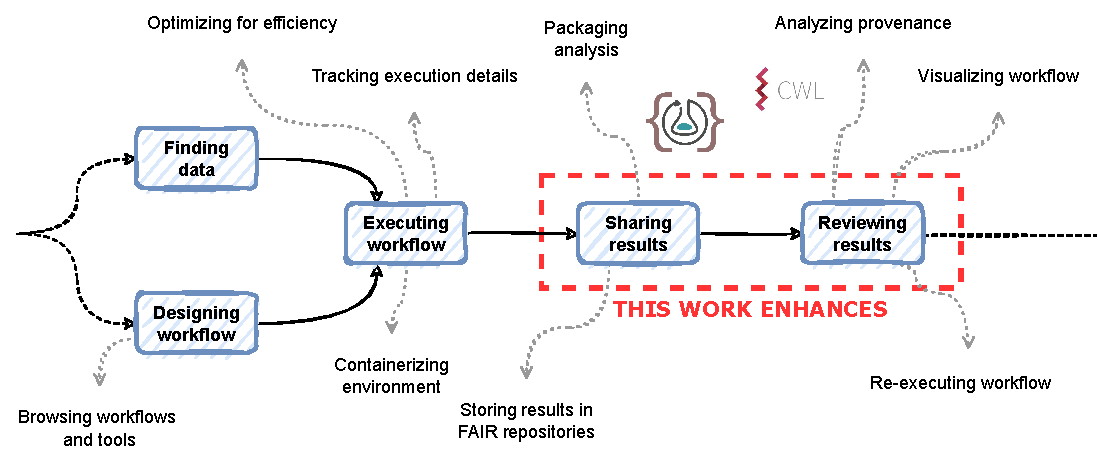
\includegraphics[width=1\textwidth]{background/vision.pdf}
    \caption{A vision of an ecosystem of workflow-related resources and its benefits for the reproducibility of computational processes. In this vision, workflows and data are stored in FAIR repositories, are executed in containerized environments by workflow systems which leverage efficient job-scheduling technologies and track details of the computation.  
    After publication, the results of the workflow can be analyzed, and workflows can optionally be re-executed as the start of new projects which build upon the research. 
    Fundamental to the success of this approach is the interoperability of the components of the ecosystem. In this work, we focus on workflow-centric Research Objects as a common format for the sharing and analysis of computational results.
    %\todorenske{Keep CWL(Prov) and ROCrate logos in?}
    }
    \label{fig:vision}
\end{figure*}
The transparency of computational analyses can be improved by expressing scientific analyses as \emph{workflows}, i.e. a series of steps with the output of one step becoming the input for another. Figure \ref{fig:vision} envisions a future in which workflows are an integral part of reproducible computational research, central to an ecosystem of tools and platforms which have emerged over the last decade. 
A crucial requirement to the success of this approach is that the workflow-related tools are compatible with each other, i.e. \emph{interoperable}. 

The problem of workflow interoperability has been partly addressed by the specification of Common Workflow Language (CWL) \citep{crusoeMethodsIncludedStandardizing2022}, a platform-neutral standard for workflow descriptions. CWL workflows are \emph{portable} across multiple workflow management systems. However, provenance of a computational result comprises more than a workflow description alone,
% a workflow description alone does not comprise the full provenance of a computational result, 
since the output data are also strongly dependent on the input configurations (data and parameter settings) and the (distributed) computational system(s) on which the workflow was executed. 


%%\stodor{Append CWLProv paragraph to wf-centric RO or separate paragraphs?} 
For this reason, workflow-centric \emph{Research Objects} (ROs) \cite{belhajjameWorkflowcentricResearchObjects2012} have been proposed as a common, machine-accessible standard for the storage and distribution of computational results. ROs are collections of resources that together contribute to a scientific result, with semantic annotations describing the aggregated entities and their relations to each other. %In addition to the workflow description, ROs may encapsulate relevant resources such as data and software, together with structured annotations describing the RO, the aggregrated entities, and their relations to each other. This preserves the interconnectedness of the generated output with both the workflow, the input data and configurations, and the system on which the workflow was executed. 


CWLProv \cite{khanSharingInteroperableWorkflow2019} is a specialization of the RO model for CWL workflows, created to show how W3C PROV-DM \cite{moreauPROVDMPROVData2013} and existing standardized vocabularies can be combined to capture workflow execution provenance. The CWL reference runner \emph{cwltool} \cite{crusoeCommonworkflowlanguageCwltool202305131557342023} can create CWLProv \emph{RO Bundles} during execution to capture the workflow description, input and output data for each step, and a machine-accessible record of the execution in RDF \cite{cyganiakRDFConceptsAbstract2014}. The tool \emph{cwlprov-py} \cite{soiland-reyesCommonworkflowlanguageCwlprovpy2022} demonstrates how to extract provenance metadata from the RO Bundle and rerun individual steps or the entire workflow.

% Here contrast 're-executability' vs 'understandability'

Although CWLProv has great potential to improve computational reproducibility and re-use, the current version of the specification only captures what happens \emph{during} workflow execution, while provenance metadata associated with the workflow inputs (if it exists) is not captured. 
One possible solution to this problem is to ask CWL users to add semantic annotations to their input data and workflows, which is already encouraged in the CWL Standards.
% For this reason, the CWL standards encourage users to add semantic annotations to their input data and workflows. 
However, in reality, the wide variety in existing metadata standards and ontologies
% metadata standards and ontologies that have been developed in recent years 
make it difficult to decide which annotations should be prioritized: the metadata captured in the RO should ultimately be able to fulfill the roles which provenance plays in practice, i.e. \emph{provenance analytics} \cite{missierLifecycleProvenanceMetadata2016}. 
Defining and understanding these purposes is also crucial for the implementation of \emph{automatic} capture of provenance metadata by workflow systems. 
Since the need for provenance may vary between scientific communities, as well as the metadata that is required to address them, it is unlikely that there exists a single standard for which provenance to capture that is both detailed enough to address domain-specific requirements and yet still applicable across a broad range of scientific disciplines. %\stodor{Nearly there. Last sentence has redundancies.} 

% Since these purposes may vary between scientific communities, as well as the metadata that is required to address them, it is challenging for workflow system developers to decide which provenance metadata should be recorded automatically.

% Therefore, it is infeasible to define a standard for provenance that is both detailed enough to address domain-specific requirements and yet still applicable across a broad range of scientific disciplines. 


% However, it can be quite intimidating to define the set of provenance metadata that is necessary to make workflows reproducible. Although there is a growing collection of standards for metadata, deciding which annotations should be prioritized for a given workflow is challenging and will vary between workflows and the purposes for which associated ROs are used. 
% As a result, workflow authors are left unsure about the reproducibility of their workflows, and it is ambiguous how provenance solutions like CWLProv can be further improved. \stodor{Rephrase last 2 sentences.}
%However, defining a standard for provenance metadata is challenging, 
% However, it is challenging to define the set of metadata which is necessary for reproducibility, given that it should be applicable across many scientific disciplines without losing important domain-specific requirements. In addition, the standard should avoid `re-inventing the wheel' and instead make use of the growing collection of metadata standards which have already been adopted by scientific communities. 

To address this problem, we describe a systematic \emph{approach} to identify the required provenance metadata for any scientific domain, and demonstrate how developers can use this information to improve existing provenance solutions. Instead of analyzing the high-level characteristics of many workflows, we decided to study a single workflow in detail, hypothesizing that the insights we would gain could also benefit workflows in other disciplines. 
We chose one exemplary bioinformatics workflow with which we were deeply familiar and defined a set of \emph{provenance questions} associated with five realistic use case scenarios. Summarizing the metadata necessary to answer the questions in a \emph{provenance taxonomy}, we analyzed how this information is captured in the current CWLProv community standard, distinguishing between different qualities of representation. Finally, we used the insights gained from our analysis to propose two extensions to CWLProv: Firstly, a set of recommendations for workflow authors to consistently annotate their input data, reusing existing, widely adopted standards. Secondly, we propose an improved representation of this metadata in CWLProv, to make it accessible for analysis with SPARQL \cite{thew3csparqlworkinggroupSPARQLOverview2013}, a query language for RDF.
% We define a set of provenance metadata specialized for one exemplary bioinformatics workflow, following a systematic approach which can be expanded to other workflows. 
% \stodor{\textbf{Important question} which we answer in this paper: How do I evaluate a RO specification (or another provenance resource that is not an RO)? Does it actually improve provenance?

% \textbf{Selling point}: Many standards have been developed, but what should we as bioinformaticians prioritize? How to apply metadata standards to our own analyses? How do we know if we are missing relevant information?}

Overall, our contribution is fourfold:
\begin{enumerate}
    \item Description of a systematic approach to identify the required provenance metadata for any workflow, summarized into a provenance taxonomy.
    \item Qualitative analysis of the CWLProv community standard with respect to this provenance taxonomy.
    \item Design of an annotation scheme for workflow authors to consistently express required metadata as annotations to their input data.
    \item Extension of the CWLProv RDF provenance graph to make more provenance metadata accessible to analysis with SPARQL.
\end{enumerate}

% \todorenske{We need to agree on the selling point. What is really the most important here?

% - The taxonomy itself (potential criticism: it is not a general standard! Only defines the provenance for one highly specialized bioinformatics workflow with a limited set of use cases).

% - The approach used to define the taxonomy (potential criticism: Well, this is quite abstract, because you only define a method, not a concrete checklist of metadata which should be included in provenance. Potentially will result in splintering, with every community doing their own thing and defining their own set of provenance metadata and designing their own solutions to represent the missing information).

% We need both components. The taxonomy itself and the framework. 
% }

% \todorenske{Selling point: Many standards have been developed, but what should we as bioinformaticians prioritize? How to apply metadata standards to our own analyses? How do we know if we are missing relevant information?}

%%\todorenske{The paper should address at least 4 audiences:

%%1. \textbf{CWL workflow authors} (`How do I make my workflow reproducible?')

%%2. \textbf{CWL developers} (`How to implement CWLProv in my workflow system?' `Can I partly automate the provenance collection to lift the burden for workflow authors?')

%%3. \textbf{Provenance experts} (`But is this the proper way to represent provenance?' --> We want to tell them that a good provenance standard requires communication with practitioners: people with real-life workflows, versionless databases and annoying provenance issues. Standard must be useful/implementable in practice.)

%%4. \textbf{General FAIR/reproducibility/... enthusiasts}: Do not use CWL/ROs but care about FAIR. May maintain databases. (`How should I design the API for my database?' `Should I send metadata during data download, and in which format?')

%%5. \textbf{Bioinformaticians} : the vast majority of workflows that are currently written do go nowhere near automated workflow, so we want to tell them to not rely on workflow systems to capture all the details, and they should start to think about that. Table 2 helps to think about all the things you should capture and worry about. Raise awareness. Figure 1 is the most important for them! Think about the entire process. 
%%}




% \section{Related work}
\label{sec:background}
\todorenske{I need feedback on the structure. Currently it is 1) Standards for metadata of workflow components, like data, software, ... 2) Standards for the relationship between the components (workflows, provenance models, ROs, 3) Previous analyses of provenance solutions. I'm mostly struggling with 3), I think there is something missing.}
% \todorenske{Not sure if this is redundant (I had to explain a lot in the introduction already). Integrate with related work section?}

In this paper, we describe the analysis and improvement of CWLProv, a standard for the preservation of CWL workflow executions. In this section, we aim to position our work into the broader context of the literature. Firstly, we discuss current standards for the preservation of data, software, and how these are linked together into workflows. We discuss the concept of workflow-centric research objects and its implementation in CWLProv. Finally, we highlight previous work on the analysis of provenance solutions based on use case analyses. 

\subsection{Metadata standards}
% Preservation of workflow building blocks is important
To achieve computational reproducibility, i.e. \emph{``the ability to obtain consistent results, using the same input data, computational steps, methods, and code; and conditions of analysis''} \cite{committeeonreproducibilityandreplicabilityinscienceReproducibilityReplicabilityScience2019}, it is firstly necessary that the individual building blocks of the analysis are preserved. Fundamental in this research area are the FAIR principles \cite{wilkinsonFAIRGuidingPrinciples2016}, which describe how data and other resources can be made Findable, Accessible, Interoperable, and Reusable, notably through their description with rich metadata in a machine-accessible format. 

In compliance with this work, scientific communities have defined their own standards for metadata. Some of these standards are applicable across many domains, such as the data \cite{datacitationsynthesisgroupJointDeclarationData2014} and software \cite{smithSoftwareCitationPrinciples2016} citation principles, while others are highly specialized towards one particular domain. 

Communities have also developed ontologies and vocabularies for the representation of this information in a machine-accessible format, such as the EDAM ontology \cite{isonEDAMOntologyBioinformatics2013}, which can be used to express concepts relevant to the field of bioinformatics. Metadata standards and ontologies are applied in dedicated data and software repositories and registries, such as bio.tools \cite{isonBioToolsRegistry2019} and Zenodo (CITE). A full overview of the landscape of metadata standards is beyond the scope of this paper and can be found in \cite{leipzigRoleMetadataReproducible2021} and on FAIRSharing.org.

\subsection{Workflow-centric research objects}
% The methods (which we require for computational reproducibility) together comprise the provenance of the results. 

The relation between different components of the analysis can be preserved through \emph{workflow thinking} \cite{grykWorkflowsProvenanceInformation2017}, i.e. dividing a computational process into a series of steps, with the output of one step becoming the input for another. Workflows can be visualized as a directed graph, where the nodes represent the operations and the edges the data flows between them.

Workflows can be described in many different ways, from simple shell scripts to dedicated workflow languages such as Snakemake (CITE) and Nextflow (CITE). Common Workflow Language \cite{crusoeMethodsIncludedStandardizing2022} is a standard for workflow descriptions which in addition to the sequence of operations (steps) also facilitates specification of software and hardware requirements and annotation of workflow (components) with metadata to make the analysis more easily understandable (Table \ref{tab:metadata_fields}). Although differences in quality certainly exist, there is currently not one workflow language which is the best option for all types of computational analyses.

\todorenske{Rephrase the last sentence ;)}

Whereas a good workflow description reflects the \emph{prospective provenance} of the results, ROs \cite{bechhoferWhyLinkedData2011} also contain \emph{retrospective provenance}. \textbf{(Which paper to cite for prospective/retrospective provenance?) } CWLProv is a specialization of the \emph{RO Bundle} serialization, an implementation of the \emph{Wf4Ever workflow-centric RO model} \cite{belhajjameWorkflowcentricResearchObjects2012}. \emph{RO Bundles} are data structures storing the CWL workflow description, input parameter file, all input and (intermediate) output data, and the provenance record describing the relations between the contained data entities and the workflow. 

To describe provenance, CWLProv adheres to the PROV-DM standard \cite{moreauPROVDMPROVData2013}. In short, PROV-DM represents the provenance record as a directed graph, in which \emph{Entities} (e.g. input files) are subjected to one or multiple \emph{Activities} (e.g. a filtering step) initiated by \emph{Agents} (e.g. a person or the workflow engine). Each of these can be further described with additional properties, often borrowed from other ontologies. For example, the \emph{wfdesc} \cite{soiland-reyesWfdescOntology2016} and \emph{wfprov} \cite{soiland-reyesWfprovOntology2016} ontologies are utilized to express workflow-specific concepts, for which the generic, domain-neutral PROV-DM vocabulary is not rich enough. The provenance graph is encoded in Resource Description Format (RDF) \cite{cyganiakRDFConceptsAbstract2014}, a machine-accessible format which can be queried with SPARQL \cite{thew3csparqlworkinggroupSPARQLOverview2013}.

Besides CWLProv, a number of other initiatives exist. The most recent of efforts is RO-Crate \cite{soiland-reyesPackagingResearchArtefacts2022}, a family of workflow language-agnostic RO specifications, which instead of the PROV ontology uses Schema.org to describe the provenance of the results. RO-Crate is defined at different levels of increasing granularity, from individual workflows, to a standard which is currently under development and was partly informed by the CWLProv specification. In addition to workflow specifications, related efforts such as BioCompute Objects also exist \cite{alterovitzEnablingPrecisionMedicine2018}. 
\todorenske{Which RO specifications are most relevant and should be included?} 

\subsection{Analysis}

Several previous efforts have defined standards and recommendations to enhance provenance, often based on selected real-life use case workflows. Firstly, Garijo et al. \cite{garijoQuantifyingReproducibilityComputational2013} attempted to reproduce a workflow published several years prior, thereby quantifying the number of hours required for scientists at 4 different levels of expertise. Based on their experience, they formulated a list of recommendations for workflow authors. 

Kanwal et al. \cite{kanwalInvestigatingReproducibilityTracking2017} applied a slightly different method in which they expressed the same workflow concept in three different languages or platforms, one of which was CWL. They identified assumptions inherent to the platforms which might compromise reproducibility at a later stage, and proposed solutions to mitigate these challenges. 

Finally, in the field of computational physics, Krafczyk et al. \cite{krafczykLearningReproducingComputational2021} composed a set of principles and associated guidelines, informed by their experience in reproducing the results of 7 publications. They also specify the Reproduction Package, a directory structure which puts the proposed principles and guidelines into practice.

How our work differs from previous work: 1) Here we analyze a specification instead of individual analyses. 2) Our approach is more systematic. 3) ??

\todorenske{Discuss content of last paragraph + rephrase.}



\begin{itemize}

    % \item \cite{samuelUnderstandingExperimentsResearch2021} maybe not worth mentioning
    % \item \cite{wittnerLightweightDistributedProvenance2022} Distributed provenance model fo complex real-world environments.
    % \item \cite{krafczykLearningReproducingComputational2021} Learning from reproducing computational results: introducing three principles and the Reproduction Package
\end{itemize}

%\section{Use case workflow}
\label{sec:workflow}

This section describes the use case workflow.

As an example case for this study, we used a previously published model for protein-protein interaction (PPI) prediction \cite{capelMultiTaskLearningLeverage2022}. However, to improve reproducibility we converted this to a workflow incorporating the calculation of the features and labels for training and prediction. 

We chose this workflow because it involves a number of elements which make reproducibility difficult. Firstly, it requires input data from databases which are continually updated. Secondly, during model development there are several different model designs that are tested, input parameter configurations and it is difficult to keep track of the versions. Also a number of tools are used with each their own versions. Another common problem: identifier mapping. Also different tools with different dependencies. Finally, this workflow is intended to be used to generate predictions for proteins for which the PPI residues are unknown, ...

\subsection{Protein-protein prediction}

Short explanation of the reason behind protein-protein prediction.

OK so why PPI prediction. Basically everything consists of proteins. Cells are made of proteins, proteins perform the critical chemical reactions in the cell. Proteins interact with each other to make this happen. They bind to each other and form complexes. What these complexes look like is very important for their function, because the shape of a protein determines what it does and what it binds to. 
It is therefore important to know the interaction sites of proteins. And also to UNDERSTAND why and how proteins interact, because structure is quite complicated.

Many diseases involve proteins with altered structure, thereby changing the functionality of the protein.

Other applications --> drug design?

Which amino acids form the \emph{protein-protein interface} can be determined from the structure of the complex: usually amino acids within a certain distance from the partner protein are labeled as PPI residues.

Resolving the structure for all complexes experimentally is infeasible. 

In principle this can be done experimentally (determine the structure of the complex), but this is both costly and time-consuming. Therefore, much effort has been devoted to predict protein structure and interaction sites, based on the protein sequence. Sequence is used to calculate a number of features.

\subsection{Structure of the workflow}

The model predicts per residue whether it is part of the protein-protein interface or not. For this purpose it utilizes a multitask learning strategy, in which besides the main task (PPI or not) the model also learns to predict a number of related structural features, such as surface accessibility. This allows the model to be trained on a larger dataset (because there is more data available about structural features than PPI) and the idea is also that it makes training faster because there is relevant information hidden in the structural information (e.g. a residue is more likely to be part of the PPI when it is on the outside of the protein). 

Besides the model, the workflow calculates a number of input features and labels used for training the model.

The input labels are derived from the (experimentally derived) protein structures, downloaded from Protein Data Bank (CITE). 

The input features are calculated based on protein sequence. These are ...

\subsection{Implementation of the workflow}

We implemented the workflow in CWL with a focus on reproducibility. 




\section{Methods and Results} 
\label{sec:taxonomy}
%% \stodor{Combines \textbf{Data Description} + \textbf{Analyses} + \textbf{Methods}; \url{https://academic.oup.com/gigascience//pages/research}}
Because metadata captured in ROs should be able to fulfill provenance requirements of real workflows, identification of these requirements is crucial to understand which metadata should be collected during execution, either by the workflow system or via manual annotations. However, due to the large variety of scientific communities and workflows, it is unlikely that a universal standard for which to capture exists which is still sufficiently detailed to capture domain-specific elements. 
% Defining a standard for provenance which is detailed enough to fulfill domain-specific requirements, yet general enough to be relevant across a broad range of scientific disciplines is challenging. 

Instead, we restricted ourselves to the detailed analysis of a single exemplary bioinformatics workflow, and formulated specific \emph{provenance questions} grounded in a set of realistic use case scenarios.
% Here, we approach this problem by examining one example real-life workflow in detail and identifying elements of the analysis that are relevant in one of the potential \emph{use case scenarios} for ROs associated with it. The resulting \emph{provenance taxonomy}
This imagination exercise gave us much insight into a set of important provenance metadata, and, summarizing it into a \emph{provenance taxonomy}, we studied the representation of each component of the taxonomy in the current CWLProv community standard. 
% \stodor{Which "its" was studied?}
Our analysis revealed that some elements of the taxonomy were insufficiently described, and that others were dependent on manual annotations of the input data and the workflow descriptions itself (for which the CWL standards were insufficiently clear); therefore our final step was to design extensions to CWLProv and guidance on manual annotations to address the gaps we had identified. 

% In summary, we take an example workflow in the field of bioinformatics and define a number of associated \emph{use case scenarios} for the results generated by one of its enactments. We synthesize a list of \emph{provenance questions} associated with each of the use cases and identify components of the analysis that should be described in the provenance record in order to answer the provenance questions. Subsequently, we classify these elements into a 6-component \emph{provenance taxonomy}. 

The rest of this section is organized as follows. Firstly, we describe the design and implementation of our exemplary workflow in CWL. Secondly, we define five realistic use case scenarios for ROs associated with the workflow. Subsequently, we synthesize a provenance taxonomy, based on a list of provenance questions grounded in each of the RO use case scenarios. Next, we describe the approach and results of our qualitative analysis of the current version of CWLProv (v0.6.0). Finally, we propose the design of two extensions to CWLProv: a scheme for annotation of workflow input data, and an extension of the provenance graph to enrich the RDF representation of the workflow execution. 

\subsection{Design and implementation of an exemplary bioinformatics workflow}
\label{sec:workflow}
\begin{figure*}[hb!]
    \label{fig:epitope_graph}
    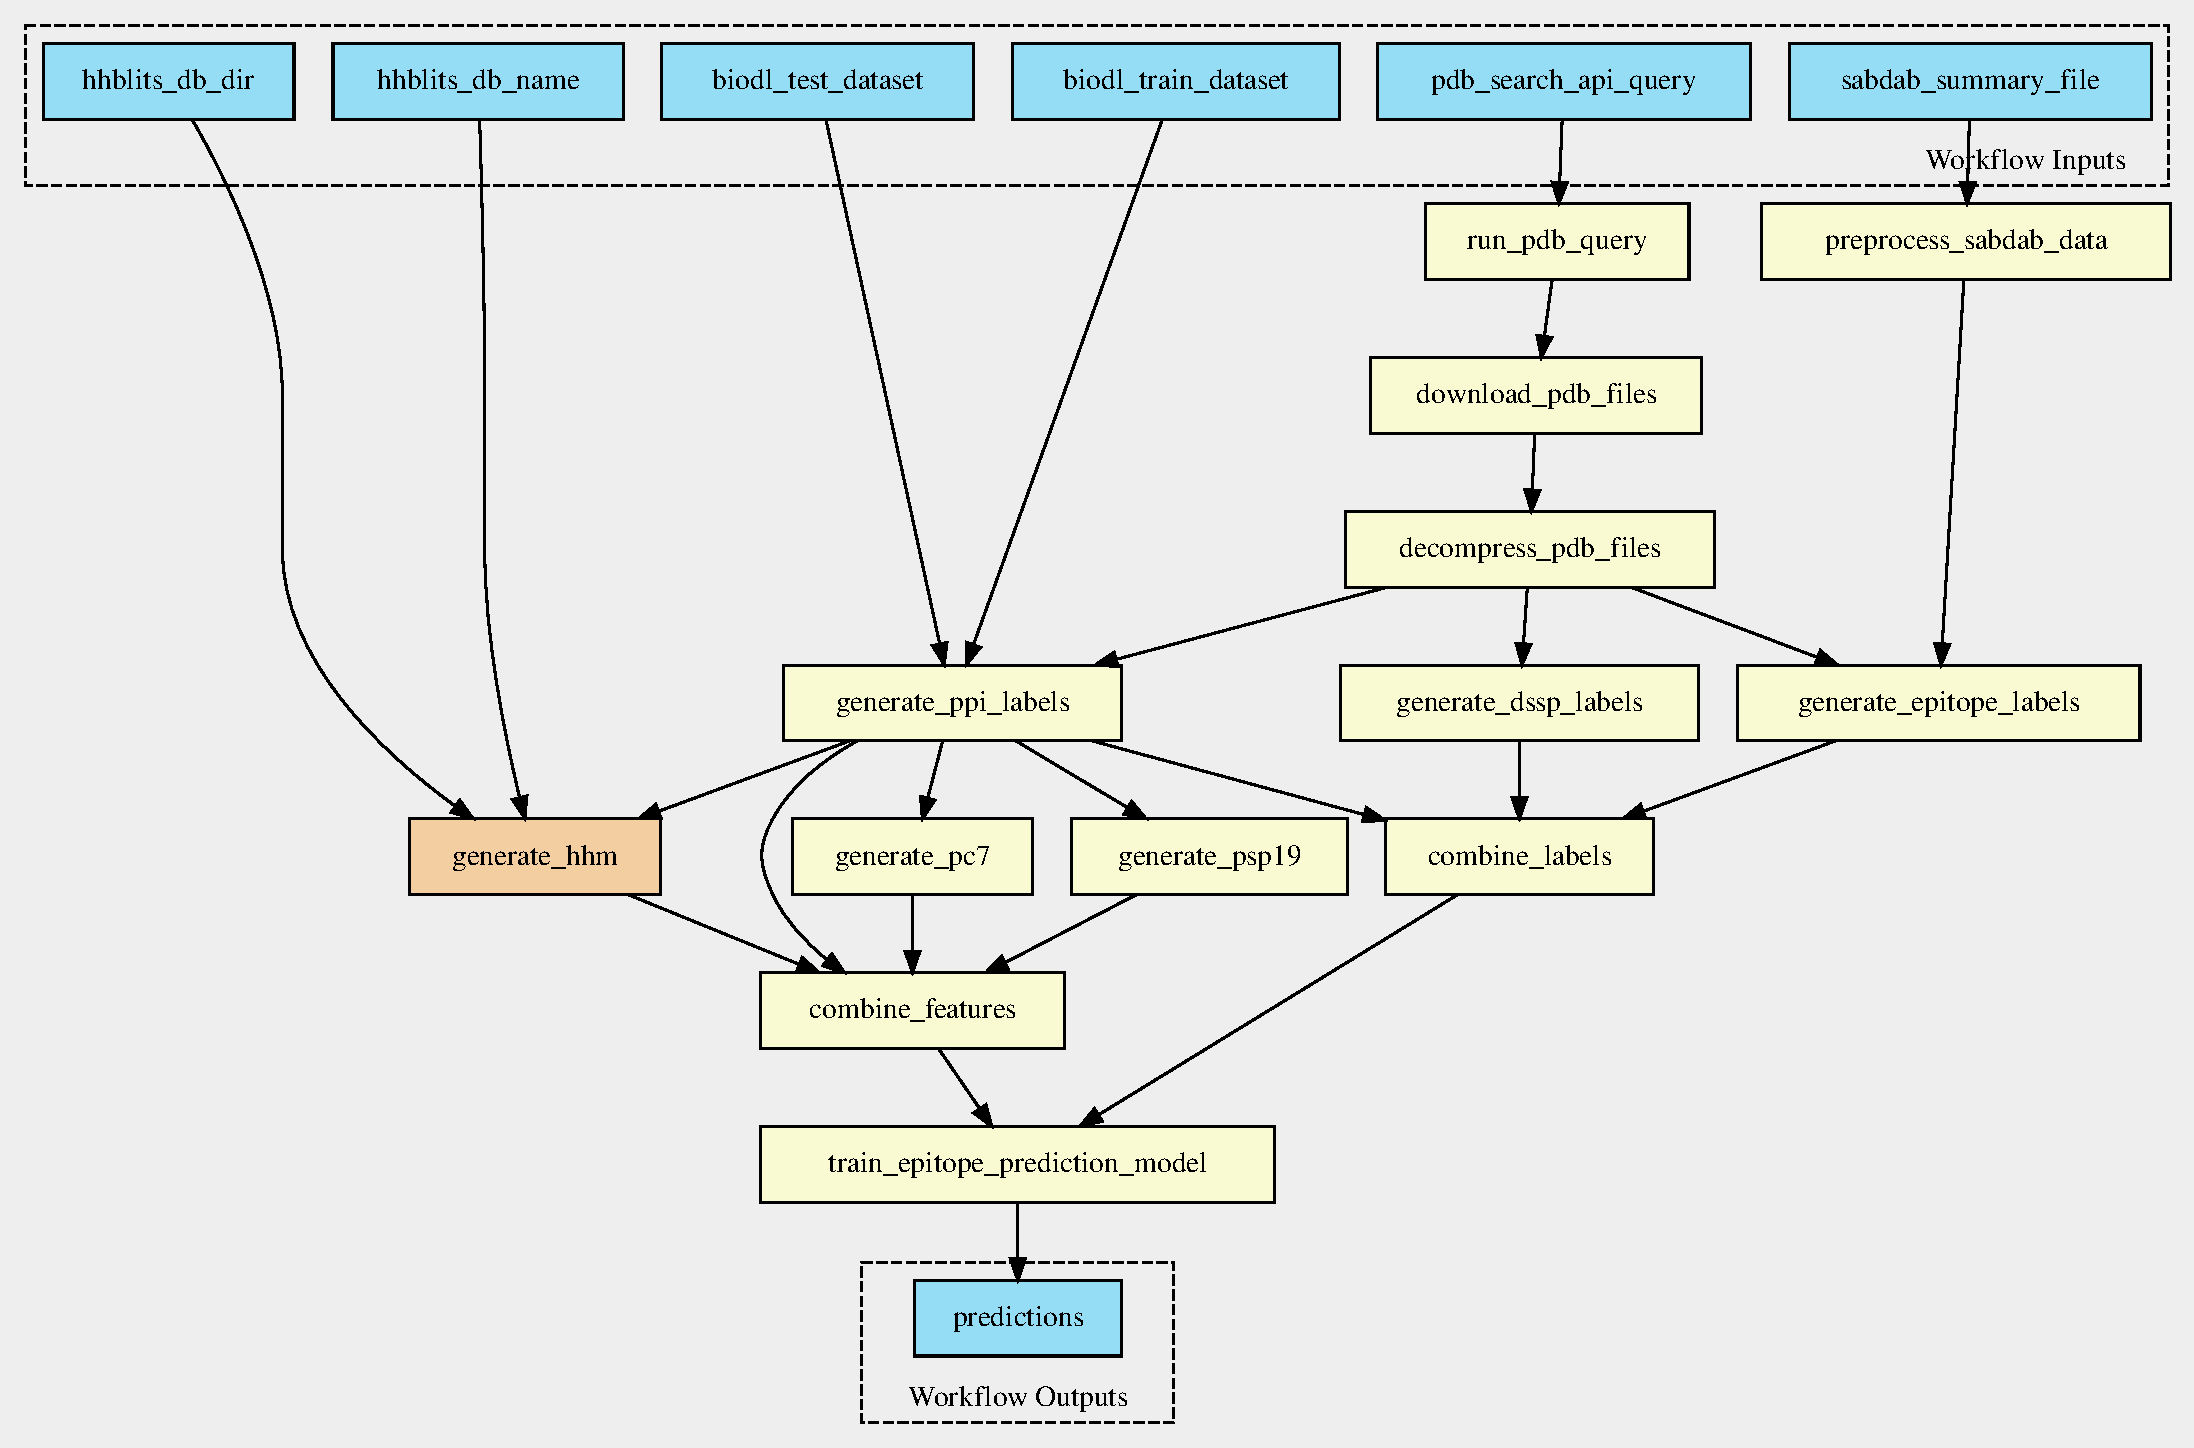
\includegraphics[width=1\linewidth]{taxonomy/workflow.pdf}
    \caption{CWL implementation of the workflow we used as an example. Based on data retrieved from multiple FAIR and non-FAIR resources, the workflow computes a set of input features and labels. These are subsequently used to train a deep learning model which predicts the amino acids in a protein which are likely to be \emph{epitopes}, i.e. binding sites for antibodies. Based on our experience, this workflow is exemplary for many problems which commonly arise when reproducing computational results.
    Nodes represent the steps, edges signify data flow between the steps. Yellow nodes indicate steps which run \emph{CommandLineTools}, orange nodes represent steps which control nested \emph{Workflows}, blue nodes signify workflow input and output parameters. }
    \label{fig:wf}
\end{figure*}
% \todorenske{We need to find a good term for this. \textit{Workflow template} was used in other publications (e.g. \citep{garijoDetectingCommonScientific2013}) for `workflow description' = the (CWL) document, which is not what we mean. \textit{Workflow motifs} are subcomponents of workflows, e.g. preprocessing \citep{garijoCommonMotifsScientific2014}. Workflow type? Workflow concept?} 


% \stodor{Explicitly reference figure 2 in the text}
As the basis of our provenance taxonomy, we used a type of bioinformatics workflow which was familiar to the authors: training a deep learning model to predict particular protein characteristics based on information encoded in the DNA. %\stodor{It is not really the DNA, but the protein sequence, but maybe this is less easy to understand.} 
More specifically, the model in our example predicts, for a given protein, which amino acids constitute \emph{epitopes}, i.e. binding sites for antibodies. Understanding antibody binding is important for e.g. vaccine design, but expensive and impractical to study experimentally because of the large number of possible protein-antibody combinations. However, the three-dimensional protein structure ultimately arises from the \emph{protein sequence}, which has been determined for a far greater number of proteins and in principle can be used to predict structural properties which are difficult to determine in the lab.
% Although this information could in principle be inferred by experimentally resolving the structure of the complex, in practice this is a difficult and expensive process and infeasible to perform for all complexes. Therefore, predictors have been developed to predict this information, based on patterns learned from protein sequence, which is encoded in the DNA and much easier to determine experimentally. 

% : training of a deep learning model on input features and labels derived from (experimental) data stored in large databases or previously published as standalone datasets. 

Based on our experience, the selected workflow has characteristics representative of many of the problems which commonly arise in reproducing computational processes. 1) It is a derived work; in our case the deep learning model is an adaptation of a previously published model for predicting general protein binding characteristics (the protein-protein interface) \cite{capelMultitaskLearningLeverage2022}. 2) Important data is the direct product of, or derived from, external databases which are continually updated and unlikely to return the same results when the same query is issued at a later date. Specifically, the property labels used to train the deep learning model are derived from experimentally resolved protein structures retrieved from large databases. 3) The workflow uses a variety of tools with specific versions, dependencies, and input parameter settings. 4) Finally, the development of this workflow involved many design choices, and many combinations of workflow steps and input configurations were tested during the search for an optimal configuration.

In our CWL description of the workflow (Figure \ref{fig:wf}), we aimed to optimize reproducibility by making some specific choices: We included database querying and data retrieval in the workflow and avoided the use of external identifier mapping tools, which are not likely to return the same output in the future. In addition, we executed most steps in software containers, and added structured annotations explaining the meaning of the workflow components and the data used as input. A detailed account of the workflow implementation can be found in the Supplementary Material (Section \emph{\nameref{sup:workflow}}). 

\subsection{Definition of Research Object use case scenarios}
\label{sec:stakeholders}

In this section, we describe the use cases of ROs associated with our example workflow coupled with the practitioners for which they are relevant. We consider five use cases, reflecting different stages in the workflow's lifetime. Some of these are applicable to workflows in most disciplines (e.g. U1), while at least one (U5) is specific to our exemplary workflow.
% \stodor{"Stages"? then use also in U3 \& U4, or nowhere. Also "stages" feel a bit linear.}

\begin{enumerate}[label=\textbf{U\arabic*}]
    \item \textbf{Workflow development}. Most relevant for: \textbf{Workflow author}. During this stage, the workflow design is not fully established. Different input datasets and configurations are tested. Steps may be added or removed based on the output of previous steps. ROs of multiple workflow runs may be used to compare different designs and configuration settings with each other. \label{uc:wf_dev}
    \item \textbf{Publishing the workflow}. Most relevant for: \textbf{Workflow author}. At this stage, the workflow is ready for publication, and the workflow author has to explain the methodology and rationale of the research in a scientific article, or write documentation for the workflow. The RO may serve as a guide during writing, comprising a record of used data and tools, contributions of collaborators (facilitating credit and attribution), and choices which were made during workflow development. \label{uc:writing}
    \item \textbf{Understanding the workflow}. Most relevant for: \textbf{Reader of the article describing the research}. This use case represents a stage in which an RO has been published in companionship with the article. The metadata contained in the RO serves as a bridge between the methods section of the article and the workflow itself. In addition, the metadata may connect the conclusions in the article to the results that support them. \label{uc:understanding}
    \item \textbf{Reproducing the workflow}. Most relevant for: \textbf{Third party continuing the research}. Follow-up stage after reading the article and examining the RO to understand the research (\ref{uc:understanding}). The RO is used as a guide to reproduce the analysis, before it is modified or extended for a new purpose. \label{uc:reproducing}
    \item \textbf{Model workflow execution as a service}. Most relevant for: \textbf{User of the trained model as a web service}. In this stage, the trained model has been made available as a web service, which can be used to predict epitopes for sequences for which the structure is unknown. An RO is the standard output format of the web-based tool. \label{uc:service}
\end{enumerate}


\subsection{Synthesis of a taxonomy of provenance}
% \todorenske{Same title as section, 1 of them should be changed.}

\label{sec:user_req}

Based on the use cases described in the previous section, we synthesized a list of \emph{provenance questions}, included in the Supplementary Material (Section \emph{\nameref{sup:provquestions}}).
Similar to the use case scenarios, we found that some questions are likely also relevant in most other domains, while others are highly specific for our workflow. Using our list of domain-informed provenance questions, we identified the metadata required to answer the questions and summarized this into a 6-component taxonomy of provenance types which should be represented in the provenance of the workflow execution: 


\begin{enumerate}[label=\textbf{T\arabic*}]
    \item \textbf{Scientific context}. Explanation of the choices which were made in the design of the workflow and parameter values. \label{tax:context}
    \item \textbf{Data}. Input and (intermediate) output data.\label{tax:data} % To explain meaning and context of the data as well as describe data not included in RO for storage, security, or privacy reasons. 
    \item \textbf{Software}. The tools directly orchestrated by the workflow, and their dependencies. \label{tax:software} % Facilitates reproduction of workflow at a later time or helps finding an alternative tool in the case of code rot. 
    \item \textbf{Workflow}. The (CWL) workflow and tool descriptions. \label{tax:wf} % Workflows are software and can be reused when published in a workflow repository.
    \item \textbf{Computational environment}. Metadata about the system on which the workflow was executed, comprising both software and hardware. \label{tax:env} % Necessary for reproduction of the workflow execution.
    \item \textbf{Execution details}. Additional information about the workflow execution itself. \label{tax:execution}
\end{enumerate}
\begin{table*}
\caption{Overview of provenance taxonomy, with the provenance questions (\emph{PQs}) that apply to each of the categories. In addition, the components of the taxonomy are integrated with already accepted principles and guidelines (\emph{Source}).
%\todorenske{What should go in Refs? Only officially defined standards like FAIR principles/data citation principles or also random publications which mention that including something may be necessary?}
}\label{tab:taxonomy}
% Use "S" column identifier (from siunitx) to align on decimal point.
% Use "L", "R" or "C" column identifier for auto-wrapping columns with tabularx.

\begin{tabularx}{\linewidth}{p{0.1in}p{0.3in}p{1.3in}Lp{0.45in}p{0.3in}} %{l{0.05\textwidth} l{0.3\textwidth} l{0.5\textwidth} L{0.05\textwidth} l{0.05\textwidth} l{0.05\textwidth}}
\toprule
{Type} & {Subtype} & {Name} & {Metadata}  & {PQs} & {Source} \\
\midrule
T1  & {SC1}\label{tax:sc1}   & Workflow design  & Annotations on the design of the workflow and its components. Purpose of the workflow, why steps were included or excluded, the meaning of particular input parameters, etc.    & 1-2, 11-12, 25-27    & \citep{committeeonreproducibilityandreplicabilityinscienceReproducibilityReplicabilityScience2019,belhajjameResearchObjectSuite2014,grykWorkflowsProvenanceInformation2017,stoddenEnhancingReproducibilityComputational2016}   \\
    & SC2   & Entity annotations                & The meaning of individual input and output data entities. Why were they chosen? How are the results interpreted?          & 1-5, 13, 28-29, 67-69  &   \\
    & SC3   & Workflow execution annotations    & Annotations about a set of parameters in a particular workflow run. Allows to distinguish between the ROs of multiple workflow runs.             & 6-7, 30-31 &  \\
\midrule
T2  & D1    & Data identification               & Persistent identifier (PID), version, name and description of the dataset. Preferred citation of the data. \emph{When the data is not FAIR:} URL and download date as an alternative for PID and version. \emph{When the dataset is a subset of a larger collection (e.g. a database):} PID of database, database version and download date, and the query or filtering strategy which produced the dataset.    & 13-16, 32-36, 47, 67-69 & \citep{datacitationsynthesisgroupJointDeclarationData2014} \\
    & D2    & File characteristics              & Filename, format, creation and last modification timestamps, size, and checksum.  & 15, 48  &  \\
    & D3    & Data access                       & URL to a downloadable form of the data. License.   &  8, 49  & \\
    & D4    & Parameter mapping                 & The workflow and step parameters for which the data is an input or output.   & 37-38 &   \\
\midrule
T3  & SW1   & Software identification           & PID, name, version, release date and description of the software. Preferred citation. \textit{When the software is not FAIR:} URL of repository, download date and/or git commit hash as substitute for PID, version or release date.       &  16-20, 50     &   \citep{smithSoftwareCitationPrinciples2016} \\
    & SW2   & Software documentation            & URL of documentation or other metadata which is important to make informed use of the tool. URL to repository with source code of the software. &  39-40, 51-52  & \\
    & SW3   & Software access                   & URL to downloadable, executable form of the software. License.               &  9, 53  & \\
\midrule
T4  & WF1   & General software metadata         & At workflow and step level, according to T3.                 & 12, 21-23, 41, 70 & \citep{gobleFAIRComputationalWorkflows2020}\\
    & WF2   & Workflow parameters               & Type, format, and description, at workflow and step-level.                & 42-44  & \\
    & WF3   & Workflow requirements             & Software and hardware resources which are required to execute the workflow or workflow steps. &  54-56  & \\
\midrule
T5  & ENV1  & Software environment              & Software (dependencies), operating system. Dependencies could comprise all installed software (might contain much redundant information if a step was not executed in a software container), or the dependencies of the software which is run (which may be difficult to identify). Should follow the requirements as described in T3.       &    57     &  \citep{committeeonreproducibilityandreplicabilityinscienceReproducibilityReplicabilityScience2019}  \\
    & ENV2  & Hardware environment              & Available RAM, storage, number and type of CPUs and GPUs. Network access.       &    58        & \\
    & ENV3  & Container image                   & Image name, tag and digest (because names and tags are not stable). Additional metadata (extracted from image labels), contents of Dockerfile (if built from Dockerfile), and general requirements for software as described in SW1.                & 24, 59-60 &  \\
\midrule
T6  & EX1   & Execution timestamps              & When the workflow was executed, at step-granularity. The timestamps can be helpful when files were downloaded during the execution, especially from a database which does not have clear versions. In addition, the duration of the execution may be important during workflow development (test different settings) and when reproducing the workflow. & 1-5, 10, 61-63 &   \\
    & EX2   & Consumed resources             & The resources used during execution, at step-granularity. This is different from what was described in WF3, because there we only described what was available, not what was actually used.  & 7, 64  &  \\
    & EX3   & Workflow engine                   & Software, therefore with same metadata as general software entities (T3).             & 45, 65 & \\
    & EX4   & Human agent                       & At a minimum, a PID such as ORCID should be included, or name and email of the person who ran the workflow. These details may be important for attribution (U2), and can also be used by third parties to ask further questions about the research.                 & 46, 66 &  \\
\bottomrule
\end{tabularx}


% \begin{tablenotes}
% \item Source is from this website: \url{https://www.sedl.org/afterschool/toolkits/science/pdf/ast_sci_data_tables_sample.pdf}
% \end{tablenotes}
\end{table*}

Each component of the taxonomy consists of several subcomponents, which are outlined in Table \ref{tab:taxonomy}.

\subsection{Qualitative analysis of the CWLProv community standard}

\label{sec:cwlprov_evaluation}

% \todorenske{Alternative title: Qualitative analysis of CWLProv  0.6.0}
% \todorenske{If we want the title to reflect the main result, what is the main result of the analysis?}
% \todorenske{Keep subheadings? }

\begin{table*}[ht!]
\caption{Summarized results of CWLProv 0.6.0 analysis. The table shows for each taxonomy component whether it is fully ($\medblacksquare$) or partially represented ($\medsquare$). Components which are not represented in any of the documents are marked with an asterisk ($\ast$). Representations which are only included when this metadata is manually supplied are indicated with parentheses. We distinguish between description in RDF, CWL-specific documents (packed.cwl, primary-job.json, and primary-output.json), and unstructured representation (e.g. execution log).}
\label{tab:analysis_res}
% Use "S" column identifier (from siunitx) to align on decimal point.
% Use "L", "R" or "C" column identifier for auto-wrapping columns with tabularx.

\begin{tabularx}{\linewidth}{l l L l l l l}
\toprule
{Type} & {Subtype} & {Name} & {structured (RDF)} & {CWL-specific} & {unstructured}  \\
\midrule
T1  & SC1   & Workflow design                   & ~    & ($\medblacksquare$) & ~  \\
    & SC2   & Entity annotations                & ~    & ($\medsquare$) & ~  \\
    & SC3   & Workflow execution annotations $\ast$   &      \\
\midrule
T2  & D1    & Data identification               & ~     & ($\medsquare$) & ~ \\
    & D2    & File characteristics              & $\medsquare$     &  ($\medsquare$)   & $\medsquare$ \\
    & D3    & Data access                       & ~ & ($\medsquare$) & ~ \\
    & D4    & Parameter mapping                 & $\medblacksquare$ & $\medblacksquare$ & $\medsquare$ \\
\midrule
T3  & SW1   & Software identification           & ~ & ($\medsquare$)  & ~  \\
    & SW2   & Software documentation            & ~ & ($\medsquare$)  & ~ \\
    & SW3   & Software access                   & ~ & ($\medsquare$)  & ~  \\
\midrule
T4  & WF1   & Workflow software metadata        & $\medsquare$ & ($\medblacksquare$)  & ~ \\
    & WF2   & Workflow parameters               & $\medsquare$ & ($\medblacksquare$)  & ~    \\
    & WF3   & Workflow requirements             & ~ & ($\medblacksquare$) & ~    \\
\midrule
T5  & ENV1  & Software environment $\ast$       & ~ & ~  & ~ \\
    & ENV2  & Hardware environment $\ast$       & ~ & ~  & ~ \\
    & ENV3  & Container image                   & $\medsquare$ & $\medsquare$ & $\medsquare$\\
\midrule
T6  & EX1   & Execution timestamps              &  $\medblacksquare$ & ~ & ~ \\
    & EX2   & Consumed resources                &  ~ & ~ & $\medsquare$ \\
    & EX3   & Workflow engine                   &  $\medsquare$ & ~ & ~    \\
    & EX4   & Human agent                       & $\medblacksquare$ & ~ & $\medblacksquare$     \\
\bottomrule
\end{tabularx}


% \begin{tablenotes}
% \item Source is from this website: \url{https://www.sedl.org/afterschool/toolkits/science/pdf/ast_sci_data_tables_sample.pdf}
% \end{tablenotes}
\end{table*}


In the previous section, we defined a set of metadata that should be included in provenance in order to meet specific use cases of ROs associated with an exemplary bioinformatics workflow. It is however also important to consider \emph{how} the metadata is included in the RO. In this section, we describe a qualitative analysis of the current CWLProv community standard (v0.6.0). %in order to decide how to extend the specification to meet the requirements associated with real-life workflows. 
We evaluated the representation of each component of the provenance taxonomy defined in the previous section, distinguishing between different qualities of representation. In later sections, we describe how we used the results of our analysis to extend the CWLProv specification to meet the requirements associated with real-life workflows.

% Now some methods of the analysis
% \subsection{Method}
% In this section, we explain the method we followed to assess CWLProv 0.6.0. 

Our analysis was based on RO Bundles generated with the CWL reference implementation \emph{cwltool}\footnote{
\mintinline{bash}|cwltool --provenance ./cwlprov_ro wf.cwl input_params.yml|
}.
% \todorenske{mention "\-\-provenance" or otherwise link to details on how this was done.}. 

% \lstinline@\verb{cwltool --provenance alsdjfl lskdfjlj lsdkjflsdkjf sdf}@
For each component of the provenance taxonomy, we evaluated the presence of the component in three levels of representation: structured representation in RDF (provenance graph and \emph{manifest.json}), structured annotations in CWL-specific documents (\emph{packed.cwl}, \emph{primary-job.json}, and \emph{primary-output.json}), and unstructured representation (e.g., the execution log). 

We also considered the amount of effort that is required to add the metadata: manual annotations require much more input from the workflow author than metadata that is automatically extracted by the workflow engine.

We considered a component \emph{fully represented} if it is included in the document by default, or if the CWL Standards provide clear guidelines for its manual annotation in a workflow or input object document. In contrast, a provenance subtype was \emph{partially represented} if only a subset of the metadata was included in the RO, or if there was ambiguity about how to represent this information in the workflow or parameter file. 
% \subsection{Requirements}
% \label{sec:analysis_reqs}
% In this analysis, we consider for each of the provenance types and subtypes defined in ?? whether they adhere to the following requirements:

% \begin{enumerate}[label=\textbf{R\arabic*}]
%     \item \label{r:rep} The provenance subtype is represented in the RO.
%     \item \label{r:struct} The representation of the subtype is in a structured format.
% \end{enumerate}

% \subsection{Methodology}
% We perform a qualitative analysis of CWLProv 0.6.0, based on ROs generated with the CWL reference implementation \textit{cwltool}. We consider each of the 6 components defined in \ref{sec:provenance_model}. We discriminate between structured representation in RDF (provenance graph and \emph{manifest.json}), structured annotations in CWL-specific documents (\emph{packed.cwl} and \emph{primary-job.json}), and \emph{unstructured} documents such as the execution log.

% We consider a component \emph{fully represented} if it is included in the document by default, or if the CWL standards provide clear guidelines for its manual annotation in a workflow or input object document. In contrast, a provenance subtype is \emph{partially represented} if only a subset of the metadata is included in the RO, or it is not clear how to annotate this in the workflow or input object document.

% \subsection{Results}
Table \ref{tab:analysis_res} summarizes the  results of the analysis.
Of all 6 provenance elements, \textbf{execution details} (\ref{tax:execution}) are best represented in CWLProv. The provenance graph contains start and end timestamps at both workflow and step granularity %\footnote{A side note to be made here is that in \emph{cwltool}-generated ROs of executions which reused cached results, the timestamps correspond to the final execution, not the original run which computed the results. We opened an issue about this: \url{https://github.com/common-workflow-language/cwltool/issues/1689} \todorenske{Keep this in?}} 
(\textbf{EX1}). The workflow engine is described with name and version (\textbf{EX3}), and linked to the human agent who initiated the workflow run (\textbf{EX4}). Apart from maximum memory used during a container execution, the RO contains no reference to used resources (\textbf{EX2}). 

The \textbf{workflow} (\ref{tax:wf}) is also represented in CWLProv. The full workflow is contained in \emph{packed.cwl}, including any structured annotations made by the workflow author (\textbf{WF1}). In contrast, the RDF description references only the workflow and its steps. Annotations are not propagated to the provenance graph, and steps are not linked to the underlying \emph{CommandLineTool} or nested \emph{Workflow} descriptions. The workflow and step execution records mention the input parameters (\textbf{WF2}) and link them to their values, but they are not further explained with metadata in the provenance graph. 
Software and hardware requirements (\textbf{WF3}) can be found in \emph{packed.cwl} if they were specified by the workflow author.

The \textbf{computational environment} (\ref{tax:env}) is very sparsely described. Only when steps are executed in a software container, the container image (\textbf{ENV3}) is represented in RDF. However, the description is restricted to its name and tag, which is not stable and does not convey any information about its contents. If an image was built from a Dockerfile, the Dockerfile is included in \emph{packed.cwl}, but there is no guarantee that the same image (with the same versions) will be built when re-executing the workflow. Other characteristics of the computational system (\textbf{ENV1}, \textbf{ENV2}) are completely absent from the provenance record.

Although the \textbf{software} (\ref{tax:software}) orchestrated by the workflow may be part of \emph{SoftwareRequirements} and therefore included in \emph{packed.cwl}, there is no guarantee that the specified versions are identical to those installed on the system which executed the workflow. If workflow authors add structured annotations about the software to the \emph{CommandLineTool} document, these are also contained in \emph{packed.cwl}. None of these annotations are represented in RDF.

In contrast to software, \textbf{data entities} (\ref{tax:data}) are represented in RDF, and linked to the workflow and step parameters for which they were values (\textbf{D4}). Each file is a separate entity in the provenance graph, and when they were part of an \emph{Array} or \emph{Directory}, this association is also described. Files are annotated in the provenance graph with filename and checksum, and \emph{manifest.json} contains the creation date of files generated during workflow execution (\textbf{D2}). However, structured annotations of input data (\textbf{D1}, \textbf{D2}, \textbf{D3}) are restricted to \emph{primary-job.json}.

The \textbf{scientific context} (\ref{tax:context}) can be partially represented by adding manual annotations in the workflow (via \emph{intent} and \emph{doc} fields, \textbf{SC1}) and input file (via custom annotations, \textbf{SC2}) and will be present in \emph{packed.cwl} and \emph{primary-job.json}. There are currently no standards for adding annotations specific for the execution (hence \textbf{SC3} is missing). 

Summarizing, we made three main observations about the CWLProv (v0.6.0) community standard. Firstly, the RDF graph is incomplete, limiting the use of SPARQL queries for analysis of the provenance. Secondly, although some of the missing metadata can be retrieved from CWL-specific documents, their presence is heavily dependent on manual annotations. The CWL Standards (v1.2) do not give detailed guidelines for the representation of annotations for input data, which is likely to increase the barrier for workflow authors to add these annotations to their workflows, and invites inconsistency when they do. Finally, there are some elements related to the execution which are missing from RDF and impractical to add as manual annotations. As a result, details about the computational environment are almost completely absent from the provenance record, compromising computational reproducibility of the workflow. 

\subsection{Proposed scheme for the annotation of input data}

% \todorenske{Given the length of the subsequent sections, would it be better to describe the 2 improvements in 1 section `Extensions to CWLProv', with separate subsections for annotation scheme, RDF extension, and `Analysis'?}

In the previous sections, we identified a set of useful provenance metadata given 5 realistic use case scenarios, summarized this into a taxonomy, and used this to perform a qualitative analysis of the current CWLProv community standard. From this analysis, we concluded that although manual annotations can be added to the workflow and parameter files to enrich the provenance, the CWL Standards do not formally specify how this information should be included. In this section, we aim to standardize the annotation of input data, proposing a scheme which enables authors to describe individual inputs as well as a complete workflow run (i.e., the combination of a particular workflow design and its configuration settings, \textbf{SC3}). 

Rather than designing our own ontology, the core vocabulary of our annotation scheme reuses the Bioschemas \citep{michelBioschemasSchemaOrg2018} \emph{Dataset} profile (v1.0), an extension of Schema.org \cite{guhaBigDataMakes2015} for life sciences. The terms listed in Table \ref{tab:dataset_bioschemas} allow authors to express generic characteristics of their input datasets, such as the identifier, version, and license. In addition, to convey information about the \emph{meaning} of the data, we recommend the use of other, domain-specific ontologies, e.g. EDAM \cite{isonEDAMOntologyBioinformatics2013}. 

In many cases, input datasets may be the result of a series of operations prior to workflow execution, from retrieval from a database to filtering and cleaning operations. We advise to encode this history as a sequence of Schema.org \emph{Actions}, each associated with their own instruments, queries, and times (Table \ref{tab:action_schemaorg}). 

% \todorenske{Add a figure with example annotation, incorporating all three features of the annotation scheme.}

Figure \ref{fig:ex_annotations} shows an example of how to apply the annotation scheme in practice. This is a parameter file with two workflow input values. The first is a standalone dataset with its own identifier and version. The second dataset is the result of a database query and subsequent filtering. The metadata is separated from the rest of the input parameters by a dedicated \emph{cwlprov:prov} field. Finally, a description of the entire workflow run is given in the root of the document.

The details of the design, as well as more extensive examples of how to apply the scheme in practice, are provided in the Supplementary Material (Section \emph{\nameref{sup:annotation}}).

\begin{figure*}[!ht]
    \centering 
    \caption{Simplified example of our annotation scheme for workflow inputs. The first input (\emph{standalone\_dataset}) is a dataset stored in a FAIR repository, with an identifier and version. The second input (\emph{filtered\_pdb\_dataset}) is the result of a database search (\emph{pdb\_search}) and subsequent filtering (\emph{filtering\_action}).}
    % \todorenske{insert structured query for pdb\_search}
    \todorenske{@Michael, is a string broken up over multiple lines (s:query; line 4-18) valid in YAML?}
    \begin{minted}[linenos,xleftmargin=\parindent, breaklines, frame=single]{yaml}
cwlprov:prov:
  pdb_search:
    s:additionalType: s:SearchAction
    s:query: "{
            'query': {
                'type': 'terminal',
                'service': 'text',
                'parameters': {
                    'attribute': 'rcsb_accession_info.deposit_date',
                    'operator': 'range',
                    'value': {
                        'from': '2010-01-01',
                        'to': '2022-08-01'
                    }
                }
            },
            'return_type': 'entry'
        }"
    s:object:
      s:identifier: https://bio.tools/pdb
    s:result: pdb_search_result
    s:endTime: 2022-08-01
    s:description: "All entries deposited between 2010 and 2022"
      
  filtering_action:
    s:additionalType: s:Action
    s:object: pdb_search_result
    s:instrument: 
      s:identifier: https://bio.tools/pisces
    s:result: filtered_pdb_dataset

filtered_pdb_dataset:
  class: Directory
  location: path://path/to/directory/
  
standalone_dataset:
  class: File
  location: path://path/to/file1.pdb
  format: edam:format_1476 # pdb
  s:identifier: https://doi.org/10.2210/pdb6nzn/pdb 
  s:version: "1.4"
  s:description: "Amyloid fibril structure of glucagon in pdb format."

s:description: "Example workflow run with 2 inputs."

$namespaces:
  s: "https://schema.org/"
  edam: "http://edamontology.org/"

$schemas:
- https://schema.org/version/latest/schemaorg-current-https.rdf
- https://edamontology.org/EDAM_1.25.owl
    \end{minted}
    \label{fig:ex_annotations}
\end{figure*}


\subsection{Proposed extension of the RDF provenance graph}
\label{sec:prov_rdf_extension}
In our analysis of CWLProv, described in the previous sections, we observed that much of the metadata was absent from the RDF representation of the execution. In this section, we describe the design and implementation of an extension to the provenance graph, in order to make more of the analysis accessible to exploration with SPARQL queries. 



Primarily, we aimed to expand the description of the workflow (i.e. \emph{prospective provenance}). Whereas the original design only mentioned the top-level workflow and its steps, the extended design incorporates all components for which the CWL Standards specify metadata fields (Table \ref{tab:metadata_fields}). In addition, provenance metadata supplied according to the annotation scheme described in the previous section is propagated to RDF. The details of the design are described in Supplementary Material (Section \emph{\nameref{sec:dev_recommendatons}}). 
% \stodor{explicitly where in the supplemental materials? with link}

We \stodor{TODO (Michael)} realized the extended design in the CWL reference implementation \emph{cwltool}. Repeating the analysis of CWLProv, we found that the extended RDF graph is notably richer in provenance metadata (Table \ref{tab:rdf_after}). Although still dependent on manual input from the workflow author, \textbf{Scientific context (\ref{tax:context})} is now fully represented in RDF, as well as \textbf{Data (\ref{tax:data})} and \textbf{Workflow (\ref{tax:wf})}. Future work should focus on the representation of workflow resource requirements, as well as computational environment. A list of SPARQL queries \stodor{TODO (Renske)} can be found in the Supplementary Material (Section \emph{\nameref{sup:sparql}}). 


\begin{table}[ht!]
\caption{RDF provenance graph after extension. The table shows for each taxonomy component whether it is fully (black) or partially represented (white), highlighting elements with improved representation in the extended design (\FiveStar). Components which are not represented in any of the documents are marked with an asterisk ($\ast$). Representations which are only included when this metadata is manually supplied are indicated with parentheses.}\label{tab:rdf_after}
% Use "S" column identifier (from siunitx) to align on decimal point.
% Use "L", "R" or "C" column identifier for auto-wrapping columns with tabularx.
% \todorenske{D2?}
% \todorenske{What about intermediate output data? Is there annotation for those possible? If not, shouldn't we change it to partial, instead of full representation?}
\begin{tabularx}{\linewidth}{l l L l }
\toprule
{Type} & {Subtype} & {Name} & {structured (RDF)} \\
\midrule
T1  & {SC1}  & Workflow design  & (\FiveStar)    \\
    & SC2   & Entity annotations                & (\FiveStar)     \\
    & SC3   & Workflow execution annotations   &  (\FiveStar)    \\
\midrule
T2  & D1    & Data identification               & (\FiveStar)     \\
    & D2    & File characteristics              & $\medsquare$ \\
    & D3    & Data access                       & (\FiveStar) \\
    & D4    & Parameter mapping                 & $\medblacksquare$  \\
\midrule
T3  & SW1   & Software identification           & ~  \\
    & SW2   & Software documentation            & ~ \\
    & SW3   & Software access                   & ~  \\
\midrule
T4  & WF1   & Workflow software metadata        & (\FiveStar) \\
    & WF2   & Workflow parameters               & (\FiveStar) \\
    & WF3   & Workflow requirements             & ~ \\
\midrule
T5  & ENV1  & Software environment $\ast$       & ~  \\
    & ENV2  & Hardware environment $\ast$       & ~ \\
    & ENV3  & Container image                   & $\medsquare$ \\
\midrule
T6  & EX1   & Execution timestamps              &  $\medblacksquare$\\
    & EX2   & Consumed resources                &  ~ \\
    & EX3   & Workflow engine                   & $\medsquare$ \\
    & EX4   & Human agent                       & $\medblacksquare$  \\
\bottomrule
\end{tabularx}


% \begin{tablenotes}
% \item Source is from this website: \url{https://www.sedl.org/afterschool/toolkits/science/pdf/ast_sci_data_tables_sample.pdf}
% \end{tablenotes}
\end{table}


%\begin{table}[bt!]
\caption{Metadata fields in CWL Standards v1.2. \emph{format} is only allowed for parameters of type File or File array.}\label{tab:metadata_fields}
\begin{tabularx}{\linewidth}{L l l l l}
\toprule
CWL field & Schema.org term \\
\midrule
% Widgets & 42 & Over-supplied\textsuperscript{*} \\
% Gadgets & 13 & Under-supplied \\
doc & description \\ %\hline
label & name \\ %\hline
format & encodingFormat \\
intent & featureList \\

\bottomrule
\end{tabularx}
\begin{tablenotes}
\item This is a table note.
\item \textsuperscript{*}Another note.
\end{tablenotes}
\end{table}


% \begin{figure*}[ht]
    \centering
    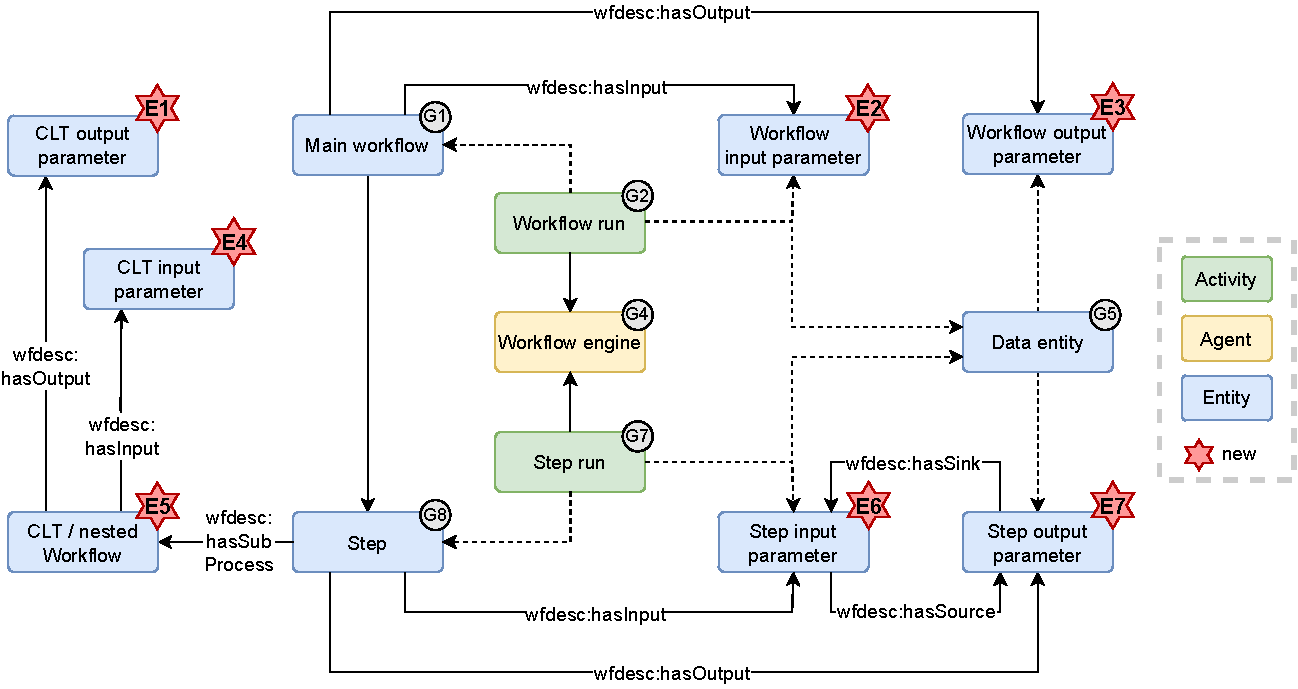
\includegraphics[width=0.99\textwidth]{rdf_extension/CWLProv_graph_extended.pdf}
    \caption{The RDF provenance graph, now extended with \emph{CommandLineTools} and parameter entities. Red stars mark nodes which are part of the design extension. Parameters are linked to their \emph{Workflow}, \emph{CommandLineTool} or step via \emph{wfdesc:hasInput} and \emph{wfdesc:hasOutput}. Node G5 represents both input and output data entities. The data flow between steps is represented via \emph{wfdesc:hasSink} and \emph{wfdesc:hasSource}. Steps are linked to their underlying tools via \emph{wfdesc:hasSubProcess}.}
    \label{fig:cwlprov_graph_new}
\end{figure*}



% \begin{figure}[ht]
    \centering
    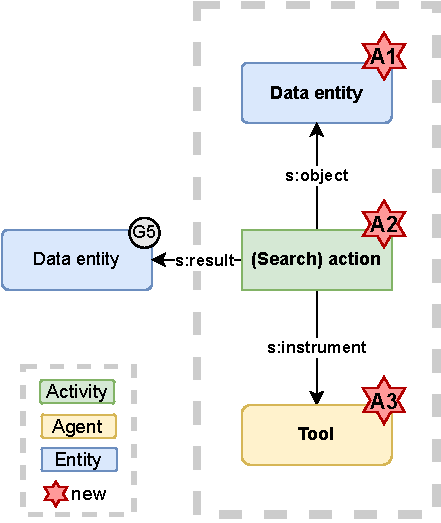
\includegraphics[width=0.4\textwidth]{rdf_extension/CWLProv_graph_extended_actions.pdf}
    \caption{Actions represented in RDF provenance graph. Workflow input datasets (\textbf{G5}) are connected to the Actions (\textbf{A2}) which produced them via \emph{s:result}. In addition, Actions can have properties such as \emph{object} (\textbf{A1}) and \emph{instrument} (\textbf{A3}).  }
    \label{fig:cwlprov_graph_actions}
\end{figure}

% \clearpage

\section{SUPPLEMENTARY}

\stodor{Replaces \textbf{Methods} section. \url{https://academic.oup.com/gigascience//pages/research}}

\section{Use case workflow}
\label{sup:workflow}
\todorenske{Text in supplementary is for a large part identical to the thesis, not paraphrased}
% \todorenske{Change `epitope' to `PPI'? Extra explanation that we adapted the PPI model to epitope prediction?}

In this section, we describe the design and implementation of our exemplary bioinformatics workflow. First, we formulate the requirements which our workflow design should fulfill. Subsequently, we provide a detailed description of our CWL implementation of the design.

\subsection{Requirements}
\label{sec:wf_requirements}


The CWL implementation of our example workflow should meet two requirements, which we explain further in the subsequent sections:

\begin{enumerate}[label=\textbf{WR\arabic*}]
    \item \label{wr:method} Adhere to a specific method of epitope prediction which was conceptualized and provided to us by the workflow authors.
    \item \label{wr:reproducibility} Address challenges which compromise the transparency and reproducibility of the workflow.
\end{enumerate}


\subsection{\ref{wr:method}: Adhere to a conceptual method}
\label{sec:wf_design}

In this section, we explain \ref{wr:method}, providing a conceptual overview of the method which should be implemented in the CWL workflow we used as an exemplary workflow in this work.

The design of the epitope predictor, conceptualized by the workflow authors, is based on a model for predicting `general' protein-protein interaction (PPI) interfaces \cite{capelMultitaskLearningLeverage2022}. In its turn, that model was derived from OPUS-TASS \cite{xuOPUSTASSProteinBackbone2020}, a predictor for protein \emph{structure}. 

It addresses the lack of training data via a multi-task learning strategy, in which the model not only learns the label of interest (epitopes), but also related characteristics, such as solvent accessibility (the fraction of amino acid surface which is exposed to the aqueous environment). This allows the model to be trained on a larger set of structures, not restricted to antibody-antigen complexes, but also including structures with general PPI interfaces and other structural information.

The PPI predictor on which this method was based, was trained on OPUS-TASS reference data and did not include calculation of the input features or labels. In contrast, the OPUS-TASS source code did contain calculation of the input features, but the labels were reused from a reference dataset and not directly derived from protein structure. \textbf{However, because we wanted to maximize the transparency of our research, our workflow comprises the entire trajectory from protein structure and sequence to labels and features used for model training.} 

\subsubsection{Data sources}
These are the (main) data sources used to calculate the input features and labels:

\begin{itemize}
    \item \textbf{Protein Data Bank (PDB)} \cite{bermanProteinDataBank2000}, a database of experimentally resolved structures of proteins and complexes.
    \item \textbf{Structural Antibody Database (SAbDab)} \cite{dunbarSAbDabStructuralAntibody2014},  a database of metadata for antibody-antigen complexes in the PDB (e.g., which part of the complex corresponds to the antibody and which to the antigen).
    \item \textbf{BioDL} \cite{stringerPIPENNProteinInterface2022}, a dataset of protein sequences containing annotations for general PPI interactions, previously derived from structure.
    \item \textbf{HHBlits reference database.} Used by HHBlits \cite{remmertHHblitsLightningfastIterative2012} to compute some of the input features.
\end{itemize}

\subsubsection{Structure-derived labels}
For each residue in each protein sequence, the model predicts a number of properties. 

\begin{itemize}
    \item \textbf{Epitope}: a binary label indicating if a given residue is an epitope. Calculated from protein structure in combination with SAbDab metadata. Missing for proteins which are not included in SAbDab.
    \item \textbf{PPI}: a binary label indicating if a given residue is part of a general PPI interface. Extracted from BioDL.
    \item \textbf{Surface accessibility}: a label indicating how much of the amino acid is exposed to the surface. Calculated by DSSP \cite{kabschDictionaryProteinSecondary1983} based on the protein structure.
    \item \textbf{Secondary structure}: 3 binary labels indicating the secondary structure of which a given residue is part (alpha helix, beta strand or loop). Calculated by DSSP based on the protein structure. 
\end{itemize}

\subsubsection{Sequence-derived input features}
The model predicts epitope annotations based on three groups of sequence-derived features:
\begin{itemize}
    \item \textbf{PC7}: 7 features which reflect amino-acid-specific physico-chemical characteristics. Every amino acid type has fixed values for these features.
    \item \textbf{PSP19}: 19 binary features which reflect the presence of particular amino acid `building blocks' (e.g. a benzene ring). Every amino acid type has fixed values for these features.
    \item \textbf{HHM}: 30 features derived from a sequence profile generated from alignment with highly similar sequences. Computed with HHBlits.
\end{itemize}

\subsection{\ref{wr:reproducibility}: Address reproducibility challenges for this workflow}
\label{sec:wf_reproducibility}

In this section, we explain \ref{wr:reproducibility} by presenting a number of characteristics of our workflow which may make its implementation challenging from a transparency and reproducibility perspective.

\subsubsection{Workflow design}

Firstly, the method requires calculation of over 50 input features and at least 6 labels for every amino acid in each of the several thousand proteins in the training dataset, involving three data sources, at least two command-line tools and several Python scripts. This underlines the importance of describing this process as a workflow, in order to keep track of all the data flows. 

Secondly, the design of the workflow is subject to extensive changes, as the workflow authors test different combinations of input features and labels in order to optimize performance as well as computational efficiency. In addition, they may need to include extra preprocessing steps to remove potential bias from the training set (e.g. due to overrepresentation of certain protein families in the PDB).

\subsubsection{Software}

The workflow steps each have their respective software dependencies, some of which are only compatible with particular versions of other software (e.g. \emph{tensorflow}). Recording the versions of tools and dependencies is therefore very important for reproducibility.

\subsubsection{Data}
Retrieving and handling the data used as input for this workflow has its own challenges. 
Firstly, HHBlits can be used with different reference databases, which will influence the produced sequence profiles. These databases have versions, and are not stored in a FAIR manner. 

Secondly, the dataset downloaded from PDB does not comprise the entire database, but a subset which is selected as the result of a query. Since new entries are added to PDB continually, it is not likely that running the same query at a later moment will result in the same dataset. Similarly, SAbDab also receives weekly updates \cite{dunbarSAbDabStructuralAntibody2014}. 

Finally, the identifiers in the BioDL dataset correspond to particular \emph{sequences}, whereas those in SAbDab and PDB represent \emph{structures}. Therefore, we need to match the two types of identifiers with each other. However, external resources such as the UniProt mapping tool\footnote{\url{https://www.uniprot.org/id-mapping/}} \cite{theuniprotconsortiumUniProtUniversalProtein2021} may not return the same mappings in the future.

\subsection{CWL implementation of the workflow}
\label{sec:wf_implementation}

In this section, we describe how we implemented the epitope prediction workflow in CWL, considering the requirements described in the previous sections. Figure \ref{fig:wf} shows an overview of the CWL implementation of the workflow.

\subsubsection{Implementation of the conceptual method (\ref{wr:method})}

To address the first requirement, the workflow starts by issuing a query to the PDB Search API\footnote{\url{https://search.rcsb.org/index.html\#search-api}} (\emph{run\_pdb\_query}). This produces a list of PDB IDs which is used to download the protein structures from PDB (\emph{download\_pdb\_files}), which are subsequently decompressed (\emph{decompress\_pdb\_files}). From the protein structures, DSSP calculates surface accessibility and secondary structure (\emph{generate\_dssp\_labels}), and an in-house Python script extracts epitope annotations (\emph{generate\_epitope\_labels}) using a SAbDab summary file which has been preprocessed in an earlier step (\emph{preprocess\_sabdab\_data}). Another Python script extracts PPI annotations from BioDL and performs identifier mapping (\emph{generate\_ppi\_labels}). Three separate steps calculate input features for the protein sequences with PPI annotations (\emph{generate\_hhm}, \emph{generate\_pc7}, and \emph{generate\_psp19}). The input features and labels are subsequently combined in two steps  (\emph{combine\_features}, \emph{combine\_labels}) and used to train the prediction model (\emph{train\_epitope\_prediction\_model}).

\subsubsection{Consideration of workflow reproducibility  (\ref{wr:reproducibility})} 
Firstly, we aimed to automate the workflow as much as possible. For this reason, the PDB query and download steps are included in the workflow (with the query as one of the workflow inputs). The two workflow inputs constituting the BioDL dataset (\emph{biodl\_test\_dataset} and \emph{biodl\_train\_dataset}) are included as remote files and downloaded by \emph{cwltool} during workflow execution. 
Because SAbDab is not programmatically accessible, \emph{sabdab\_summary\_file} needs to be downloaded manually, but all further preprocessing steps are included of the workflow. 

To avoid using external mapping tools between UniProt and PDB identifiers, we infer the relationships between the two types of IDs from the downloaded PDB files, which contain both types of identifiers. 

To make the workflow design easy to adapt and modify with different combinations of input features and labels, we spread the computation of these features over separate steps. This is different from the original OPUS-TASS code, in which all input features are calculated by a single Python script. 

To increase the portability of the computational environment, some steps are executed inside software containers. The workflow engine pulls Docker images from external repositories and converts them to Singularity \cite{kurtzerSingularityScientificContainers2017} containers, the software which is installed on the Bazis HPC cluster on which we executed the workflow. 
% Steps for which there was no image available can be containerized in the future by building custom images from Dockerfiles and uploading them to our own repository.

\subsubsection{Emulation of workflow steps} 
Because this workflow is still in development, some steps are emulated. In this way, the steps produce output in the expected format, but do not necessarily contain biologically sensible information. 

In summary, for three steps we used scripts provided by the workflow authors (\emph{preprocess\_sabdab\_data}, \emph{generate\_epitope\_labels}, and \emph{generate\_dssp\_labels}). For other steps we reused or modified code from OPUS-TASS (\emph{generate\_pc7}, \emph{generate\_psp19}, and \emph{generate\_hhm}) or other sources (\emph{run\_pdb\_query}, \emph{download\_pdb\_files}). Finally, we wrote custom Python scripts for the remaining steps, of which two were partially (\emph{combine\_labels}) or completely emulated (\emph{train\_epitope\_prediction\_model}). 

\clearpage
\section{Provenance questions}\label{sup:provquestions}

% \todorenske{How to organize this section? Idea 1: leave it as it is. Idea 2: Make sideways table with 1 question per row, add columns for each use case (U1 - U5) and provenance subcomponent (SC1, SC2, SC3, D1, ...). Indicate for which use case and provenance component each question is applicable. }

\newlist{provquestions}{enumerate}{1}
\setlist[provquestions, 1]
{label=Q\arabic{provquestionsi}., %1., 2., 3., ...
leftmargin=2\parindent,
rightmargin=10pt
}


\subsection*{\ref{uc:wf_dev}: Workflow development}

\begin{provquestions}
    \item What is the influence of including filtering step X on performance? (SC1, SC2, EX1)
    \item What is the influence of a different model architecture on performance? (SC1, SC2, EX1)
    \item What is the influence of a different training set on performance? (SC2, EX1)
    \item What is the influence of a different value for input parameter X on performance? (SC2, EX1)
    \item What is the influence of removing model training feature X on performance? (SC2, EX1)
    \item What is the difference between workflow runs X and Y? (SC3)
    \item Which of workflow runs X and Y used more RAM? (SC3, EX2)
    \item Under which conditions am I allowed to reuse this third-party dataset as input for my workflow? (D3)
    \item Under which conditions am I allowed to reuse this third-party software tool for my workflow? (SW3)
    \item What is the influence of ... on training time? (EX1)
\end{provquestions}

\subsection{\ref{uc:writing}: Publishing the workflow}
\begin{provquestions}[resume]
    \item On which previous research was this research built (conceptually)? (SC1)
    \item Which of my colleagues contributed to the conceptualization of this research? What were their contributions? (SC1, WF1, EX4)
    \item Which cleaning operations were performed on workflow input X? (SC2, D1)
    \item Which were all the datasets I used as inputs and should be cited? (D1)
    \item When was dataset X downloaded from database Y? (D1, D2)
    \item What are all the resources which contributed to this research (and should be cited)? (D1, SW1)
    \item Which software was used in this workflow? (SW1)
    \item I reused a custom, unpublished script made by one of my collaborators. How do I give credit to the original authors? (SW1)
    \item I wrote a custom script based on existing code. How do I give credit to the original authors? (SW1)
    \item I wrote a CWL \emph{CommandLineTool} description for existing software. How do I cite it? (SW1)
    \item I reused an existing CWL CommandLineTool description. How do I give credit to the original authors? (WF1)
    \item Which of my colleagues contributed to this workflow to whom I should give credit and/or propose as co-authors? What were their contributions? (WF1)
    \item From which workflow(s) was this workflow derived? (WF1)
    \item I reused a Dockerfile or Docker container image which was written or built by someone else. How do I give credit to the original authors? (ENV3)
\end{provquestions}

\subsection{\ref{uc:understanding}: Understanding the workflow}
\begin{provquestions}[resume]
    \item What is the goal of this analysis? (SC1)  
    \item Why was this step included? (SC1)
    \item Why was this combination of steps chosen? (SC1)
    \item What is the interpretation of this (intermediate) output?  (SC2)
    \item What was the performance of the model? (SC2)
    \item What was the hypothesis of this workflow run? (SC3)
    \item Why was this set of values chosen as inputs for this workflow execution? (SC3)
    \item Where can I find more information about BioDL dataset? (D1)
    \item Which SAbDab query was used to generate the summary file? (D1)
    \item Which UniProt IDs are part of BioDL? (D1)
    \item Which query was issued to PDB? (D1)
    \item How was this figure from the paper generated? (D1)
    \item For which workflow parameter is this dataset an input? (D4)
    \item Which workflow step produced this output file? (D4)
    \item What was the model architecture? (SW2)
    \item Which related tasks were predicted by the model? (SW2)
    \item How were UniProt IDs mapped to PDB IDs? (WF1)
    \item Which input features were used for the model? (WF2)
    \item What are the values of PSP19 for each amino acid type? (WF2)
    \item What is the format of this output file? (WF2)
    \item How should I cite \emph{cwltool}? (EX3)
    \item Who can I contact for more information about the research? (EX4)
\end{provquestions}

\subsection{\ref{uc:reproducing}: Reproducing the workflow}

\begin{provquestions}[resume]
    \item Which HHBlits reference database was used? Which version? (D1)
    \item What was the last modification date of this input file? (D2)
    \item Where can I download HHBlits reference database? (It was not stored in the RO because of its large size.) (D3)
    \item Which version of HHBlits was used? (SW1)
    \item The CWL \emph{CommandLineTool} description did not describe all parameters of this command-line program. Which values were used for the other parameters? (SW2)
    \item Which format does the PDB batch download script need? (SW2)
    \item Where can I download HHBlits? (SW3)
    \item Does this step need network access? (WF3)
    \item How many CPUs are required for this step, according to the workflow description? (WF3)
    \item How much RAM is necessary for this step, according to the workflow description? (WF3)
    \item Which software (and their versions) was installed on the system? (ENV1) 
    \item Which CPU/GPU was installed? (ENV2)
    \item Original author used Dockerfile. Is the image I built on a rerun the same as the one in the original analysis?  (ENV3)
    \item I pulled a Docker image. Is this the same as which was used in the original analysis? (ENV3)
    \item How long does this step take? (EX1)
    \item When was PDB database queried? (EX1)
    \item When was SAbDab database queried? (EX1)
    \item How much memory was used in the original run? (EX2)
    \item Which version of \emph{cwltool} was used in the original run? (EX3)
    \item Who ran the original workflow and how can I contact them for more information? (EX4)
\end{provquestions}

\subsection{\ref{uc:service}: Model as a web service}

\begin{provquestions}[resume]
    \item What was the query which returned the set of proteins for which I made predictions with the model? (SC2, D1)
    \item Which protein sequences were in the training set? (SC2, D1)
    \item Which proteins had epitope annotations? (SC2, D1)
    \item How should I cite this tool? (WF1)
\end{provquestions}

\clearpage
\section{Annotation scheme}
\label{sup:annotation}


\subsection{Requirements} \label{sec:annot_req}

Based on the results of the analysis described in Section \emph{\nameref{sec:cwlprov_evaluation}}, the input annotation scheme should meet the following requirements:

\begin{enumerate}[label=\textbf{IR\arabic*}]
    \item \label{ir:metadata} Represent the elements defined in \textbf{D1} and \textbf{D3}.
    \item \label{ir:types} Describe input data of type \emph{File}, \emph{Directory} and \emph{Array}.
    \item \label{ir:history} Represent the history of processed input data (e.g filtering).
    \item \label{ir:query} Represent the database query which produced a dataset.
    \item \label{ir:extend} Support extension with domain-specific vocabularies.
    \item \label{ir:context} Represent information about a set of input parameters (\textbf{SC3})
\end{enumerate}

\subsection{Design principles}
\label{sec:annot_principles}

The design of the input data annotation scheme was based on a set of underlying principles:

\begin{enumerate}[label=\textbf{IP\arabic*}]
    \item \textbf{Reuse of existing terms and ontologies.} Our scheme uses Schema.org, since this complies with the Bioschemas \cite{grayPotatoSaladProtein2017} initiative. Schema.org terms are also adopted by related efforts such as the RO-Crate specification \cite{soiland-reyesPackagingResearchArtefacts2022}. \label{pr:bioschemas}
    \item \textbf{Extension of the CWL standards only when absolutely necessary.} We started from the latest CWL Standards specification (v1.2), and only where these did not support adding metadata we proposed an extension. \label{pr:current_standards}
    \item \textbf{Clear separation between input data and metadata.} This keeps the input object document relatively easy to understand. \label{pr:separate}
    \item \textbf{Simplicity.} The annotation scheme should be easy to understand and use for CWL workflow authors. \label{pr:simplicity}
\end{enumerate}

\subsection{Annotations supported by CWL standards v1.2}
\label{sec:annot_cwl_now}
Here, we explain the annotations that are supported by the latest release of the CWL standards (\ref{pr:current_standards}). In the examples outlined below, we abbreviate \emph{\url{http://schema.org/}} with the prefix \emph{s:}.

\subsubsection{Format}
CWL Standards v1.2 support semantic annotations for \emph{File} and \emph{Directory} objects in the input object document. We recommend that annotations are appended on the same level as the standard fields (\emph{class}, \emph{location} and \emph{format}), where the property is the key and the annotation itself the value. Values can be single annotations, arrays or (arrays of) dictionaries. 

In addition, the authors can convey information about a \emph{set} of input parameters via annotations in the root of the input object document (\ref{ir:context}). 

\subsubsection{Vocabulary}
Information about a set of input values can be expressed under the \emph{s:description} key. 

For \emph{File} and \emph{Directory} inputs, we reused the Bioschemas Dataset profile v1.0\footnote{\url{https://bioschemas.org/profiles/Dataset/1.0-RELEASE}}, in this way complying with \ref{pr:bioschemas}. 
Table \ref{tab:dataset_bioschemas} shows how the Schema.org terms relate to the required metadata specified in \textbf{D1} and  \textbf{D3}. 

We recommend that authors adhere to this vocabulary when describing properties of their datasets which are domain-neutral. However, if they want to convey domain-specific information which is not covered by the terms in Table \ref{tab:dataset_bioschemas}, they may choose to extend this annotation scheme with domain-specific ontologies (such as EDAM \cite{isonEDAMOntologyBioinformatics2013}), in this way fulfilling \ref{ir:extend}. 

In Section \emph{\nameref{sec:sup_example_annotations}}, we show some annotation examples. In general, we recommend that authors provide at a minimum the metadata which is not covered by the identifier of the data they use (\ref{pr:simplicity}). 

\begin{table}[bt!]
\caption{Schema.org terms to use to express the metadata elements described in \ref{tax:data}. Taken from Bioschemas Dataset profile v1.0.}\label{tab:dataset_bioschemas}
\begin{tabularx}{\linewidth}{l l L}
\toprule
Schema.org & T2 element & Expected type \\
\midrule
        identifier & PID & URL \\ %\hline
        version & version & Number, Text \\ %\hline
        name & name & Text \\ %\hline
        description & description & Text \\ %\hline
        citation & citation & CreativeWork \\ %\hline
        includedInDataCatalog & database & DataCatalog \\ %\hline
        dateCreated & download date & Date, DateTime \\ %\hline
        dateModified & modification date & Date, DateTime \\ %\hline
        distribution & URL to data & DataDownload \\ %\hline
        license & license & URL \\ %\hline
\bottomrule
\end{tabularx}
\end{table}
\begin{table}[bt!]
\caption{Schema.org terms to represent the history of data inputs.}\label{tab:action_schemaorg}
\begin{tabularx}{\linewidth}{l l L}
\toprule
Schema.org & Expected type & Explanation \\
\midrule
% Widgets & 42 & Over-supplied\textsuperscript{*} \\
% Gadgets & 13 & Under-supplied \\
query & Text & Query used (only for SearchAction) \\ %\hline
object & Thing & Database or initial dataset \\ %\hline
result & Thing & Resulting dataset \\ %\hline
instrument & Thing & Tool used, e.g. for filtering \\ %\hline
endTime & DateTime, Time & Time of action \\ %\hline
agent & Organization, Person & Who performed the action \\ %\hline
description & Text & Description of the action \\ %\hline
\bottomrule
\end{tabularx}
\end{table}



\subsection{Proposed extension of CWL standards to support richer annotations.}
\label{sec:annot_new_cwl}

The previous section explained how the latest release of the CWL standards can support metadata annotations. However, with the presented annotation scheme, authors will find it difficult to explain the history of processed input data in a structured format (\ref{ir:history}). In addition, it is non-trivial to explain that a dataset (which can be a collection of files) is the result of a database query (\ref{ir:query}).

In this section, we propose an extension to the CWL standards which enables authors to annotate \emph{Arrays} (\ref{ir:types}), and represent queries and processing operations which lead to the dataset they used as input for the workflow execution.

\subsubsection{Format.} 

We propose that authors represent the history of their datasets as a sequence of actions in the input object document. These actions are performed on an initial dataset and produce a result. The result of an action can be the input of another.

To avoid obfuscating the input object document, the metadata must be listed under a \emph{cwlprov:prov} field, separate from the input values (\ref{pr:separate}). This is analogous to the \emph{overrides} field in the current CWL standards
\footnote{\RaggedRight\url{https://cwltool.readthedocs.io/en/latest/##overriding-workflow-requirements-at-load-time}}.% have to double the # to escape it

\subsubsection{Vocabulary.}

We used Schema.org terms to express search and processing actions. Table \ref{tab:action_schemaorg} lists the properties defined for \emph{s:Actions} and (more specific) \emph{s:SearchActions} and explains how they can be used in the annotation of CWL documents. In general, \emph{Actions} are performed on an \emph{object}, producing a \emph{result}. The action can be initiated by an \emph{agent}, using an \emph{instrument}. \emph{SearchActions} can be based on a \emph{query}. The moment the action was performed can be represented via \emph{endTime}.

\onecolumn
\subsection{Example input annotations}
\label{sec:sup_example_annotations}

\subsubsection{Annotations for a FAIR file.}
\label{sec:annot_fair}
The following is an example of a standalone dataset with its own identifier. In addition to the CWL-specific \emph{format} field (\emph{line 4}), we provided additional Schema.org terms in order to comply with \ref{ir:metadata}. In principle, providing the identifier and version with a description (\emph{lines 5-7}) is sufficient for unambiguous identification, since the identifier resolves to a landing page with additional information. However, for the purpose of our example, we added all other terms from Table \ref{tab:dataset_bioschemas} manually as well (\emph{lines 8-16}).

\begin{minted}[linenos,xleftmargin=\parindent, breaklines]{yaml}
FAIR_file:
  class: File
  location: path://path/to/6nzn.pdb
  format: http://edamontology.org/format_1476 # pdb
  s:identifier: https://doi.org/10.2210/pdb6nzn/pdb 
  s:version: "1.4"
  s:description: "Amyloid fibril structure of glucagon in pdb format."
  s:name: "6NZN"
  s:citation: 
    s:identifier: https://doi.org/10.1038/s41594-019-0238-6
  s:dateCreated: 2019-02-14
  s:dateModified: 2019-12-18 
  s:includedInDataCatalog: # PDB
    s:identifier: https://doi.org/10.25504/FAIRsharing.2t35ja
  s:distribution: https://ftp.wwpdb.org/pub/pdb/data/structures /divided/pdb/nz/pdb6nzn.ent.gz
  s:license: https://spdx.org/licenses/CC0-1.0
\end{minted}

\subsubsection{Annotations for a file without persistent identifier} \label{sec:annot_nonfair}
% \Cref{sup:annot_nonfair} 

When the dataset is not FAIR, the download or modification date (\emph{line 7}) can serve as an alternative for version. The URL of the remote file is used as an alternative to a persistent identifier (\emph{line 3}).

\begin{minted}[linenos,xleftmargin=\parindent, breaklines]{yaml}
nonFAIR_file:
  class: File
  location: https://www.ibi.vu.nl/downloads/PIPENN/PIPENN/BioDL-Datasets/prepared_biolip_win_p_testing.csv
  format: http://edamontology.org/format_3752 # csv
  s:additionalType: s:Dataset 
  s:name: "BioDL test set"
  s:dateModified: "2021-08-02" # an alternative to version
  s:citation:
    s:identifier: https://doi.org/10.1093/bioinformatics/btac071
  s:license: https://spdx.org/licenses/GPL-3.0-or-later.html
  s:description: "BioDL test set containing only protein-protein interactions."
\end{minted}


\subsubsection{Adding domain-specific annotations.}

The CWL standards also support adding domain-specific ontologies. Here we add extra information about the biological interpretation of the data, using terms from the EDAM ontology (with \emph{edam:} for  \emph{http://edamontology.org/}). In addition to the identifier, version and description (\emph{lines 5-7}), we explicitly define this file as a dataset and protein structure (\emph{lines 8-10}) and express the scientific domain to which it is related (\emph{line 11}). 

\begin{minted}[linenos,xleftmargin=\parindent, breaklines]{yaml}
domain_annotations_file:
  class: File
  location: path://path/to/6nzn.pdb
  format: http://edamontology.org/format_1476 # pdb
  s:identifier: https://doi.org/10.2210/pdb6nzn/pdb 
  s:version: "1.4"
  s:description: "Amyloid fibril structure of glucagon in pdb format."
  s:additionalType:
  - s:Dataset
  - edam:data_1460 # protein structure
  edam:has_topic: edam:topic_2814 # protein structure analysis
\end{minted}

\subsubsection{Annotation of a collection of input parameters.} \label{sec:annot_actions}
This example shows how scientific context can be represented, even for parameters which are not \emph{Files} or \emph{Directories}. Lines 1-5 denote the value of the workflow input parameters. The entire set of parameters is described via \emph{s:description} (\emph{line 7}), providing a mechanism to distinguish ROs of different workflow runs from each other.

\begin{minted}[linenos,xleftmargin=\parindent,breaklines]{yaml}
input1: "string value"
input2: 4
input3:
  class: File
  location: path://path/to/file.txt

s:description: "Workflow run without input feature X to test effect on model performance."
\end{minted}

\subsubsection{Example annotation of a sequence of actions.} 

In the following example, a database search was performed (\emph{lines 2-8}), followed by a filtering operation (\emph{lines 10-15}). The resulting dataset was used as an input for the workflow (\emph{lines 17-19}). Both actions are listed under \emph{cwlprov:prov} (\emph{line 1}). The result of the search action (\emph{line 7}) corresponds to the object of the filtering operation (\emph{line 12}). In this example, the query is provided in a human-readable format, but the exact query which was issued (a JSON string) could also be used.

\begin{minted}[linenos,xleftmargin=\parindent,breaklines]{yaml}
cwlprov:prov:
  pdb_search:
    s:additionalType: s:SearchAction
    s:query: "All proteins with at least 2 chains deposited between 2010 and 2022"
    s:object:
      s:identifier: https://bio.tools/pdb
    s:result: pdb_search_result
    s:endTime: 2022-08-01
      
  filtering_action:
    s:additionalType: s:Action
    s:object: pdb_search_result
    s:instrument: 
      s:identifier: https://bio.tools/pisces
    s:result: filtered_pdb_dataset

filtered_pdb_dataset:
  class: Directory
  location: path://path/to/directory/
\end{minted}

\subsubsection{Annotation of a merged dataset}

In this example, a dataset is constructed from two other datasets (\emph{lines 4-6}).
Here, the instrument is not a tool but a function (\emph{line 7})

\begin{minted}[linenos,xleftmargin=\parindent,breaklines]{yaml}
cwlprov:prov:
  merge_action:
    s:additionalType: s:Action
    s:object:
    - dataset1
    - dataset2
    s:instrument: pd.merge(dataset1, dataset2, on = "ID", how = "inner")
    s:result: merged_dataset
    s:description: "Imported both datasets as pandas dataframes, performed inner merge and saved as csv."

merged_dataset:
  class: File
  location: path://path/to/file.csv
\end{minted}

\subsubsection{Annotation of exemplary bioinformatics workflow}
Below, we show how we applied our annotation scheme to the input file for our example workflow. We represented the download action which produced the \emph{sabdab\_summary\_file} (\emph{lines 2-13}). If files were not downloaded during workflow execution, we supplied the URL to the dataset using \emph{s:distribution} (\emph{line 69}). Every file has a citation (\emph{s:citation}), consisting of the DOI of the primary publication. Finally, we supplied EDAM annotations to each \emph{File} and \emph{Directory} input (\emph{lines 29, 44, 58, 72}) and annotated the workflow run (\emph{line 78}). 
\begin{minted}[linenos,xleftmargin=\parindent,breaklines]{yaml}
cwlprov:prov:
  sabdab_search:
    s:additionalType: s:SearchAction
    s:query: "All structures"
    s:endTime: 2022-05-27
    s:object:
      s:additionalType: s:DataCatalog
      s:name: "Structural Antibody Database"
      s:citation:
        s:identifier: https://doi.org/10.1093/nar/gkab1050
    s:result: sabdab_summary_file
    s:description: "Search Action for metadata on antibody-antigen complexes in SAbDab"
    s:additionalType: edam:operation_0339 # structure database search

pdb_search_api_query:
  class: File
  location: path://path/to/pdb_query.json
  format: iana:application/json
  s:description: "Input query for PDB search API."
  s:additionalType:
  - edam:data_3786 # Query script

sabdab_summary_file:
  class: File
  path: path://path/to/sabdab_summary_all_20220527.tsv
  format: iana:text/tab-separated-values
  s:description: "Summary file downloaded from SAbDAb database, containing metadata for all structures."
  s:additionalType:
  - edam:data_2080 # database search results
  - s:Dataset
      
biodl_train_dataset:
  class: File
  location: https://www.ibi.vu.nl/downloads/PIPENN/PIPENN/BioDL-Datasets/prepared_biolip_win_p_training.csv
  format: http://edamontology.org/format_3752 # csv
  s:description: "BioDL training set containing PPI annotations for protein sequences (UniProt IDs)"
  s:name: "BioDL training dataset"
  s:dateModified: 2021-08-04
  s:citation:
    s:identifier: https://doi.org/10.1093/bioinformatics/btac071
  s:license: https://spdx.org/licenses/GPL-3.0-or-later.html
  s:additionalType:
  - s:Dataset
  - edam:data_1277 # protein features

biodl_test_dataset:
  class: File
  location: https://www.ibi.vu.nl/downloads/PIPENN/PIPENN/BioDL-Datasets/prepared_biolip_win_p_testing.csv
  format: http://edamontology.org/format_3752 # csv
  s:description: "BioDL test set containing PPI annotations for protein sequences (UniProt IDs)."
  s:name: "BioDL test dataset"
  s:dateModified: 2021-08-04
  s:citation:
    s:identifier: https://doi.org/10.1093/bioinformatics/btac071
  s:license: https://spdx.org/licenses/GPL-3.0-or-later.html
  s:additionalType:
  - s:Dataset
  - edam:data_1277 # protein features

hhblits_db_dir: 
  class: Directory
  location: path://path/to/uniclust30_2018_08/
  s:citation:
    s:identifier: https://doi.org/10.1038/nmeth.1818
  s:name: "uniclust30_2018_08_hhsuite"
  s:version: "2018_08"
  s:description: "Directory containing HHBlits reference database."
  s:license: https://spdx.org/licenses/CC-BY-SA-4.0
  s:distribution: https://wwwuser.gwdg.de/~compbiol/uniclust/2018_08/uniclust30_2018_08_hhsuite.tar.gz
  s:additionalType:
  - s:Dataset
  - edam:data_0955 # data index

hhblits_db_name: "uniclust30_2018"

hhblits_n_iterations: 1

s:description: "Demonstration run of epitope prediction workflow. Some steps are emulated, so the results of the workflow are not yet biologically meaningful."

$namespaces:
  iana: "https://www.iana.org/assignments/media-types/"
  s: "https://schema.org/"
  edam: "http://edamontology.org/"

$schemas:
- https://schema.org/version/latest/schemaorg-current-https.rdf
- https://edamontology.org/EDAM_1.25.owl
\end{minted}


\clearpage
\twocolumn
\section{Design of an extension of the CWLProv provenance graph}
\label{sec:dev_recommendatons}

\begin{figure*}[ht]
    \centering
    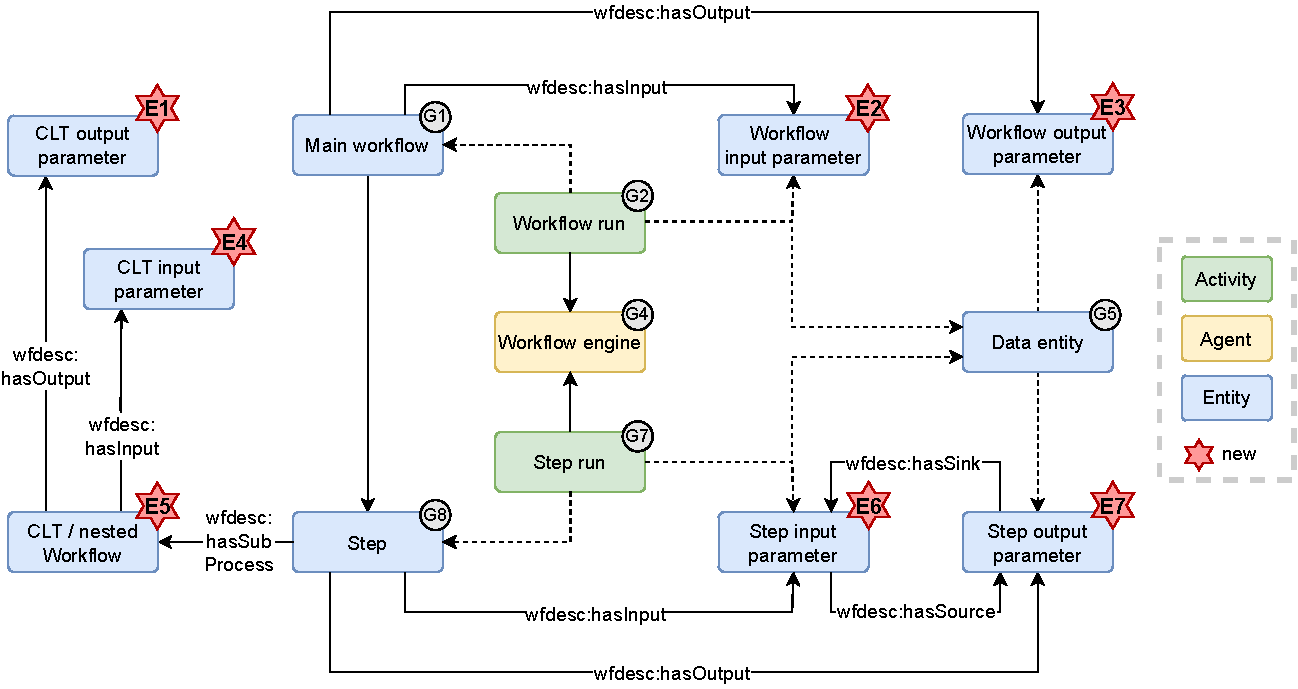
\includegraphics[width=0.99\textwidth]{rdf_extension/CWLProv_graph_extended.pdf}
    \caption{The RDF provenance graph, now extended with \emph{CommandLineTools} and parameter entities. Red stars mark nodes which are part of the design extension. Parameters are linked to their \emph{Workflow}, \emph{CommandLineTool} or step via \emph{wfdesc:hasInput} and \emph{wfdesc:hasOutput}. Node G5 represents both input and output data entities. The data flow between steps is represented via \emph{wfdesc:hasSink} and \emph{wfdesc:hasSource}. Steps are linked to their underlying tools via \emph{wfdesc:hasSubProcess}.}
    \label{fig:cwlprov_graph_new}
\end{figure*}



\begin{figure}[ht]
    \centering
    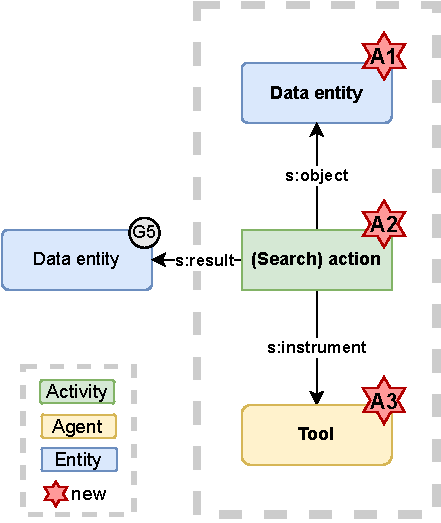
\includegraphics[width=0.4\textwidth]{rdf_extension/CWLProv_graph_extended_actions.pdf}
    \caption{Actions represented in RDF provenance graph. Workflow input datasets (\textbf{G5}) are connected to the Actions (\textbf{A2}) which produced them via \emph{s:result}. In addition, Actions can have properties such as \emph{object} (\textbf{A1}) and \emph{instrument} (\textbf{A3}).  }
    \label{fig:cwlprov_graph_actions}
\end{figure}

In Section \emph{\nameref{sec:cwlprov_evaluation}}, we analyzed CWLProv for the representation of the provenance taxonomy we defined in \emph{\nameref{sec:user_req}}. Based on this analysis, we concluded that not all provenance components were sufficiently represented in a structured format. Specifically, we found that although certain metadata was part of \emph{primary-job.json} and \emph{packed.cwl}, these annotations were not represented in RDF format.

In this section, we propose an extension of the design of the CWLProv provenance graph, which can at least represent the values for already supported metadata fields and can also be extended later with other metadata. %In this way, we (partially) answer \ref{rq:improve}.

Here, we are only concerned with the representation of this information, if it exists. Mechanisms for the collection of the metadata (whether it be manually or automated), are considered out of scope for this paper. 

In Section \emph{\nameref{sec:ext_reqs}}, we first describe the requirements and principles which we used in this design. Subsequently, in Section \emph{\nameref{sec:ext_overview}}, we give a high-level overview of the design. We then give recommendations for specific terms and vocabulary which can be used for the metadata fields \emph{doc}, \emph{label}, \emph{intent}, and \emph{format} which are part of v1.2 of the CWL Standards (Section \emph{\nameref{sec:ext_details}}). We describe how we have partially realized this design in \emph{cwltool} (Section \emph{\nameref{sec:realization}}). Finally, we provide a list of SPARQL queries in Section \emph{\nameref{sup:sparql}}.
\stodor{keep the analysis in?}

\subsection{Requirements and principles}
\label{sec:ext_reqs}
For this design, we reuse principles \ref{pr:bioschemas} and \ref{pr:current_standards}. In addition, the RDF extension should adhere to four requirements.

\begin{enumerate}[label=\textbf{PR\arabic*}]
    \item \label{pr:metadata_fields} Represent the annotations that are supported in CWL workflows according to the CWL standards v1.2, summarized in Table \ref{tab:metadata_fields}.
    \item \label{pr:input} Represent the annotations for \emph{Files} and \emph{Directories} proposed in Section \emph{\nameref{sec:annot_cwl_now}}.
    \item \label{pr:execution} Represent the annotations for a collection of input values proposed in Section \emph{\nameref{sec:annot_cwl_now}}.
    \item \label{pr:actions} Represent the annotations for Actions proposed in Section \emph{\nameref{sec:annot_new_cwl}}.
\end{enumerate}

\subsection{High-level overview}
\label{sec:ext_overview}
In this section, we present a high-level overview of the extended provenance graph and link it to the requirements defined in Section \emph{\nameref{sec:ext_reqs}}.

\subsubsection{Representation of CWL metadata fields}

\begin{table}[bt!]
\caption{Metadata fields in CWL Standards v1.2. \emph{format} is only allowed for parameters of type File or File array.}\label{tab:metadata_fields}
\begin{tabularx}{\linewidth}{L l l l l}
\toprule
Workflow component & label & doc & intent & format \\
\midrule
% Widgets & 42 & Over-supplied\textsuperscript{*} \\
% Gadgets & 13 & Under-supplied \\
Workflow & \textbullet & \textbullet & \textbullet & ~\\ %\hline
WorkflowStep & \textbullet & \textbullet & ~ & ~\\ %\hline
CommandLineTool & \textbullet & \textbullet & \textbullet & ~\\ %\hline
ExpressionTool & ~ & ~ & \textbullet & ~\\ %\hline
WorkflowInputParameter & \textbullet & \textbullet & ~ & \textbullet\\ %\hline
WorkflowOutputParameter & \textbullet & \textbullet & ~ & \textbullet\\ %\hline
WorkflowStepInput & \textbullet & ~ & ~ & ~\\ %\hline
WorkflowStepOutput & ~ & ~ & ~ & ~\\ %\hline
CommandInputParameter & \textbullet & \textbullet & ~ & \textbullet\\ %\hline
CommandOutputParameter & \textbullet & \textbullet & ~ & \textbullet\\ %\hline
\bottomrule
\end{tabularx}
\end{table}

Figure \ref{fig:cwlprov_graph_new} shows how we extended the provenance graph to represent all current metadata fields (\ref{pr:metadata_fields}). \textbf{In the new graph, every workflow component in Table \ref{tab:metadata_fields} is represented as a distinct entity, and interrelated with terms from the \emph{wfdesc} ontology (\ref{pr:bioschemas}).} 
We added entities describing the CWL tools that are run by the steps (\textbf{E5}) and linked them to their input (\textbf{E4}) and output parameters (\textbf{E1}) via \emph{wfdesc:hasInput} and \emph{wfdesc:hasOutput}. We connected the steps (\textbf{G8}) and tools via \emph{wfdesc:hasSubProcess}. In addition, we linked the step parameters (\textbf{E6}, \textbf{E7}) together via \emph{wfdesc:hasSource} and \emph{wfdesc:hasSink} to express the data flow between the steps.

In CWLProv 0.6.0, the execution of nested workflows is described in separate RDF documents. \textbf{Following the same strategy, we recommend to only represent top-level parameters of nested workflows in the primary provenance graph.} More detailed annotations can be represented in the separate RDF documents which describe the nested workflows.

\subsubsection{Representation of input data annotations}
This structure depicted in Figure \ref{fig:cwlprov_graph_new} also supports representation of the input data annotations described in \emph{\nameref{sec:annot_cwl_now}} (\ref{pr:input}), by transferring them to the data entities they describe (\textbf{G5}). 


\subsubsection{Representation of configuration settings annotations} Annotations describing a collection of parameters (\ref{pr:execution}) are specific to the workflow execution. Therefore, we recommend that these annotations are transferred to the entity in the provenance graph describing the workflow execution (\textbf{G2}).

\subsubsection{Representation of input data history}
In the annotation scheme described in Section \emph{\nameref{sec:annot_new_cwl}}, the history of (processed) input data is expressed through \emph{Actions}. Figure \ref{fig:cwlprov_graph_actions} presents their representation in RDF (\ref{pr:actions}). 
Actions (\textbf{A2}) are performed on objects, which are data entities not aggregated in the CWLProv RO (\textbf{A1}). Actions can have additional properties such as Tools (\textbf{A3}) or other annotations as summarized in Table \ref{tab:action_schemaorg}. They are connected to input data entities (\textbf{G5}) via \emph{s:result}. 



\subsection{Details of the design}
\label{sec:ext_details}
Here, we move from the structure of the provenance graph to the annotations that now can be attached to the newly added entities and with which terms they should be represented.

First, we describe which terms to use for the CWL-specific metadata fields \emph{doc}, \emph{label}, \emph{format}, and \emph{intent}.

Although we could use the exact terms with \emph{cwlprov} prefix, we aim for interoperability with other provenance representations, such as the RO-Crate specification. Therefore, we reuse Schema.org terms, and because this is in agreement with our annotation scheme:

\begin{itemize}
    \item \textbf{doc}: http://schema.org/description
    \item \textbf{label}: http://schema.org/name
    \item \textbf{format}: http://schema.org/encodingFormat
    \item \textbf{intent}: http://schema.org/featureList
\end{itemize}

\textbf{In addition, we recommend that custom annotations attached to workflow components and input objects are transferred as they are.} We make an exception for \emph{s:additionalType}, for which the value can be added to the \emph{types} of the entity it describes, instead of being literally transferred as \emph{s:additionalType}.

When entities are described with nested annotations (e.g. \emph{s:citation}), we recommend to make this a separate entity in the graph instead of a nested annotation, in compliance with the PROV data model (\ref{pr:bioschemas}).

\subsection{Partial realization in \emph{cwltool}}
\label{sec:realization}
\todorenske{Update, when this is published there should be full support in cwltool.}
Because of time constraints, we could only partially realize the provenance graph extension in \emph{cwltool}. At the time of writing, annotations directly associated with inputs of type \emph{File} and \emph{Directory}, as exemplified in \emph{\nameref{sec:annot_fair}}, are propagated to the RDF provenance record. However, annotations of the collection of input parameter values (\emph{\nameref{sec:annot_actions}}) or annotations under \emph{cwlprov:prov} (\emph{\nameref{sec:annot_new_cwl}}), are currently not represented in RDF.

\subsection{Conceptual analysis of the design extension}
\label{sec:ext_analysis}

\todorenske{leave in?}
To test the extended design, we analyzed the RDF provenance graph which would have been associated with the epitope prediction workflow we used as an example in this thesis. The elements of the design which were not yet realized in \emph{cwltool}, we emulated via manual annotations of the document. 

\subsubsection{SPARQL queries.}

\todorenske{replace with all sparql queries}
Here, we present two example SPARQL queries we issued on the emulated extended provenance graph. The first (\textbf{Q1}) extracts the DOIs of all publications which were the citations of the used inputs.

The second (\textbf{Q2}) lists the formats for every file for which this is specified.

\clearpage
% \section{Taxonomy}

\subsection{\ref{tax:context}: Definition of metadata for scientific context}
\label{sec:reasoning_reqs}

In ??, we presented scientific context (\ref{tax:context}) as one of the aspects that should be present in the collected provenance. In this section, we elaborate on what we mean with scientific reasoning and how it should be incorporated in provenance.

\textbf{Why:} Representing the scientific thinking process in provenance is meant to make the connection between the article advertising the research and the research itself, contained in the RO. This connection is bidirectional: ROs can be used as a guide during manuscript writing as well as for providing context for a third party who has read the paper and wants to understand the analysis in more depth.

\textbf{What:} The scientific context covers many aspects of the research, from the reasons why particular input data and parameter settings were chosen \cite{committeeonreproducibilityandreplicabilityinscienceReproducibilityReplicabilityScience2019}, to the design of the workflow (why particular steps were included), to the rationale for the study and the overall hypothesis of the research \cite{belhajjameResearchObjectSuite2014}\cite{grykWorkflowsProvenanceInformation2017}. Even negative results can be reported and explored strategies which did not work can be included \cite{stoddenEnhancingReproducibilityComputational2016}. In addition, it can include the interpretation of the results and their implications on the field (or maybe the output of an intermediate step warrants the inclusion of another preprocessing step).

\textbf{How:} We classify scientific context into 3 components:
\begin{enumerate}[label=\textbf{SC\arabic*}]
    \item \textbf{Workflow design}. Annotations on the design of the workflow and its components. Purpose of the workflow, why steps were included or excluded, the meaning of particular input parameters, etc. \label{req:sr_wf}
    \item \textbf{Entity annotations}: The meaning of individual input and output data entities. Why were they chosen? How are the results interpreted? \label{req:sr_data}
    \item \textbf{Workflow execution annotations}: Annotations about a set of parameters in a particular workflow run. Allows to distinguish between the ROs of multiple workflow runs. \label{req:sr_ex}
\end{enumerate}

% \subsection{\ref{tax:data}: Definition of metadata for data}
\label{sec:data_reqs}

In this section, we describe which metadata should be attached to data entities (\ref{tax:data}) in the provenance record. 

\textbf{What:} We mean not only input data, but also (intermediate) output data.

\textbf{Why:} Metadata associated with data entities can have at least two purposes:
\begin{itemize}
    \item \textbf{To explain the meaning and context of the data.} The context of the data should be described, because others need to be able to assess the appropriateness of the data for the purpose of the computational analysis. \textit{In the case of the epitope prediction workflow, it is important to understand the composition of the training set, since this is highly influential on the performance and applicability of the model.}
    \item \textbf{To describe data which is not contained in the RO.} To reduce RO size, or because the data cannot be shared for privacy reasons (it is proprietary or in other ways non-public), data may not be present in the RO but stored in an external repository. Characteristics of the data may still be included which provide information, to make sure that the data in the repository is the same as which was used in the original analysis. \textit{Use case \ref{uc:service} is an example where limiting the size of the RO may be desirable. Instead, the RO could contain references to datasets which are too large and are instead stored in an external repository.}
\end{itemize}

\textbf{How:} We identify 4 categories of data metadata which should be represented based on these two reasons. Here we link them to established recommendations and best practices for data citation, according to the FORCE11 Data Citation Principles \cite{datacitationsynthesisgroupJointDeclarationData2014}, which are based on the FAIR principles \cite{wilkinsonFAIRGuidingPrinciples2016}.

\begin{enumerate}[label=\textbf{D\arabic*}]
    \item \textbf{Identification}: PID, version, name and description of the dataset. Preferred citation of the data. \emph{When the data is not FAIR:} URL and download date as an alternative for PID and version. \emph{When the dataset is a subset of a larger collection (e.g. a database):} PID of database, database version and download date, and the query or filtering strategy which produced the dataset. \label{req:data_id}
    \item \textbf{File characteristics}: Filename, format, creation and last modification timestamps, size, and checksum. \label{req:data_char}
    \item \textbf{Access}: URL to a downloadable form of the data. License. \label{req:data_access}
    \item \label{req:data_mapping} \textbf{Mapping}: The workflow and step parameters for which the data is an input or output.
\end{enumerate}

% \subsection{\ref{tax:software}: Definition of metadata for software}
\label{sec:software_reqs}

In this section, we elaborate on the representation of software in the provenance record (\ref{tax:software}). 

\textbf{What:} In particular, we mean the command-line programs directly orchestrated by the workflow. However, these principles also apply to the workflow itself (\Cref{sec:wf_reqs}), the workflow engine (\Cref{sec:execution_reqs}), and computational environment (\Cref{sec:env_reqs}).

\textbf{Why:} There are two main reasons why software should be described with metadata:

\begin{itemize}
    \item \textbf{Obtaining identical results in a re-execution may be highly dependent on the version of the tools used.} This is important when reproducing the workflow. 
    \item \textbf{The original software may not be available or executable in the future.} In this case, the software should be sufficiently described for others to choose a suitable equivalent. 
\end{itemize}

\textbf{How}: We identify 3 categories of software characteristics which should be included in the provenance. Here we link them to established recommendations and best practices for software citation, according to the FORCE11 Software Citation Principles \cite{smithSoftwareCitationPrinciples2016}, which were adapted from the FORCE11 Data Citation Principles.

\begin{enumerate}[label=\textbf{SW\arabic*}]
    \item \textbf{Identification}: PID, name, version, release date and description of the software. Preferred citation. \textit{When the software is not FAIR:} URL of repository, download date and/or git commit hash as substitute for PID, version or release date. \label{req:sw_id}
    \item \textbf{Documentation}: URL of documentation or other metadata which is important to make informed use of the tool. URL to repository with source code of the software. \label{req:sw_doc}
    \item \textbf{Access}: URL to downloadable, executable form of the software. License. \label{req:sw_access}
\end{enumerate}


% \subsection{\ref{tax:wf}: Definition of metadata for workflow}
\label{sec:wf_reqs}

In this section, we describe the metadata that is associated with the workflow (\ref{tax:wf}). 

\textbf{What}: We define workflow here as the documents described in CWL (for other workflows, this would be the top-level script, not the underlying software that it controls). Hence the workflow comprises the main workflow description and the \emph{CommandLineTool} and nested \emph{Workflow} descriptions. 

\textbf{Why}: Workflows provide both a high-level overview of the analysis as well as details which are difficult to convey in a textual format in the Methods section of a scientific article \cite{gilAutomatingDataNarratives2017}. In addition, workflows are software which should be preserved and reused \cite{gobleFAIRComputationalWorkflows2020}. 

\textbf{How}: The metadata associated with workflows comprise general software metadata, in addition to workflow-specific information. 
\begin{enumerate}[label=\textbf{WF\arabic*}]
\item \textbf{General software metadata}: At workflow and step level, according to \Cref{sec:software_reqs}. \label{req:wf_all}
\item \textbf{Parameters}: Type, format, and description, at workflow and step-level. \label{req:wf_param}
\item \textbf{Requirements}: Software and hardware resources which are required to execute the workflow or workflow steps. \label{req:wf_resources}
\end{enumerate}


% \subsection{\ref{tax:env}: Definition of metadata for computational environment}
\label{sec:env_reqs}

In this section, we describe the requirements for computational environment (\ref{tax:env}).

\textbf{What}: Environment encompasses both software and hardware infrastructure, and may be part of a software container.

\textbf{Why}: Information about the computational environment is important for reproducing the workflow (\ref{uc:reproducing}). 

\begin{itemize}
    \item \textbf{Required resources:} Details about the resources available on the system which executed the original analysis can give an indication of what is necessary to rerun the workflow, even if this is not documented in the workflow description.
    \item \textbf{Debugging:} The generated output (or executability) of a step may be sensitive to specific versions of the tool orchestrated by the step or its dependencies.
\end{itemize}

\textbf{How}: We discriminate between three components of the computational environment:
\begin{enumerate}[label=\textbf{ENV\arabic*}]
    \item \textbf{Software}: software (dependencies), operating system. Dependencies could comprise all installed software (might contain much redundant information if a step was not executed in a software container), or the dependencies of the software which is run (which may be difficult to identify). Should follow the requirements as described in \Cref{sec:software_reqs}. \label{req:env_software}
    \item \textbf{Hardware}: Available RAM, storage, number and type of CPUs and GPUs. Network access. \label{req:env_hardware}
    \item \textbf{Container image}: Image name, tag and digest (because names and tags are not stable). Additional metadata (extracted from image labels), contents of Dockerfile (if built from Dockerfile), and general requirements for software as described in \Cref{sec:software_reqs}. \label{req:env_image}
\end{enumerate}

% \subsection{\ref{tax:execution}: Definition of metadata for execution details}
\label{sec:execution_reqs}

In this section, we define the final element of our provenance taxonomy: execution details (\ref{tax:execution}).

\textbf{What}: Executions are everything that is related to the analysis but which is not covered by the other categories. They constitute pure retrospective provenance: a record of what actually happened during the workflow run. 

\textbf{How}: We distinguish four components in this category:

\begin{enumerate}[label=\textbf{EX\arabic*}]
    \item \textbf{Timestamps}: When the workflow was executed, at step-granularity. The timestamps can be helpful when files were downloaded during the execution, especially from a database which does not have clear versions (SAbDab). In addition, the duration of the execution may be important during workflow development (test different settings) and when reproducing the workflow. \label{req:ex_time}
    \item \textbf{Consumed resources}: The resources used during execution, at step-granularity. This is different from what was described in \Cref{sec:env_reqs}, because there we only described what was available, not what was actually used. \label{req:ex_resources}
    \item \textbf{Workflow engine}: Software, therefore with same metadata as general software entities (\Cref{sec:software_reqs}).\label{req:ex_engine}
    \item \textbf{Human agent}: At a minimum, a PID such as ORCID should be included, or name and email of the person who ran the workflow. These details may be important for attribution (\ref{uc:writing}), and can also be used by third parties to ask further questions about the research.  \label{req:ex_human}
\end{enumerate}


\onecolumn
\section{SPARQL queries}
\label{sup:sparql}

\subsection{How to run the queries}

\begin{verbatim}
import rdflib
from rdflib.plugins.sparql import prepareQuery
from rdflib.namespace import Namespace
import pandas as pd

def run_query(rdf_file, query_file, namespaces):
    """
    rdf_file = RDF file; query_file = path to sparql query file; namespaces = Namespace object for every prefix in the SPARQL query.
    """
    g = rdflib.Graph()
    g.parse(rdf_file)
    with open(query_file, 'r')  as f:
        query_string = f.read()
        query = prepareQuery(
            queryString = query_string,
            initNs = namespaces,
        )

    print(f"SPARQL QUERY IS:\n{query}")
    
    qres = g.query(query)
    
    results = pd.DataFrame(qres.bindings).map(str).rename(columns=str)
    return results

def extract_wf_namespace(rdf_file):
    """
    Function which extracts namespace from CWLProv RDF provenance graph.
    """
    g = rdflib.Graph()
    g.parse(rdf_file)
    namespaces = list(g.namespaces())
    wf_namespace = ""
    for ns in namespaces:
        (prefix, namespace) = ns
        if prefix == "wf":
            wf_namespace = namespace

    return wf_namespace

provenance_file = "/path/to/provenance/file.ttl"
query_file = "/path/to/sparql/query/file.sparql" # file with any of the SPARQL queries listed in the section below

SCHEMA = Namespace("http://schema.org/")
WFDESC = Namespace("http://purl.org/wf4ever/wfdesc#")
wf_namespace = extract_wf_namespace(provenance_file)

namespaces = {"wf": wf_namespace, 
              "wfdesc": WFDESC,
              "schema": SCHEMA }

# How to run the query
response = run_query(provenance_file, query_file, namespaces)
\end{verbatim}

\subsection{SPARQL queries}

\noindent
\textbf{Return the \emph{doc}, \emph{label} and \emph{intent} fields of the main workflow.}

\lstinputlisting[basicstyle=\footnotesize]{sparql_queries/queries/wf_metadata_fields.sparql}

\noindent
\textbf{List \emph{doc} and \emph{label} fields of all \emph{WorkflowSteps} in the main workflow.}


\lstinputlisting[basicstyle=\footnotesize]{sparql_queries/queries/wf_step_metadata_fields.sparql}

\noindent
\textbf{Return the \emph{doc}, \emph{label} and \emph{intent} fields of every command-line tool or nested workflow that is run by each of the steps.}

\lstinputlisting[basicstyle=\footnotesize]{sparql_queries/queries/clt_nested_wf_metadata_fields.sparql}

\noindent
\textbf{List \emph{doc}, \emph{label}, \emph{format} fields of all input parameters of main workflow.}

\lstinputlisting[basicstyle=\footnotesize]{sparql_queries/queries/wf_input_params_metadata_fields.sparql}

\noindent
\textbf{List \emph{doc}, \emph{label}, \emph{format} fields of all output parameters of main workflow.}

\lstinputlisting[basicstyle=\footnotesize]{sparql_queries/queries/wf_output_params_metadata_fields.sparql}

\noindent
\textbf{List \emph{doc}, \emph{label}, \emph{format} fields of all input parameters of nested \emph{Workflows}/\emph{CommandLineTools}.}

\lstinputlisting[basicstyle=\footnotesize]{sparql_queries/queries/clt_nested_wf_input_params_metadata_fields.sparql}

\noindent
\textbf{List \emph{doc}, \emph{label}, \emph{format} fields of all output parameters of nested \emph{Workflows}/\emph{CommandLineTools}.}


\lstinputlisting[basicstyle=\footnotesize]{sparql_queries/queries/clt_nested_wf_output_params_metadata_fields.sparql}



\section{Discussion}
\stodor{Combines \textbf{Discussion} + \textbf{Potential implications} sections; \url{https://academic.oup.com/gigascience//pages/research}}
To facilitate reuse of computational research, there is an urgent need for a common, machine-accessible format for sharing the results of computational analyses. CWLProv \cite{khanSharingInteroperableWorkflow2019} is an RO specification that encapsulates both data and provenance metadata associated with workflow executions.
However, the wide choice in metadata standards and ontologies can make it difficult for practitioners and developers to \emph{prioritize} a set of useful metadata that should be collected during workflow execution.
Here we describe an approach to define such a set of metadata by focusing on relevant provenance questions grounded in a limited set of use cases for one exemplary workflow, instead of a high-level analysis of many workflows in a particular discipline. 
% Here we address this problem by defining provenance metadata that is required to answer a set of provenance questions grounded in five realistic use case scenarios for one exemplary bioinformatics workflow. 
% However, because requirements for provenance vary between communities and purposes for which the provenance is used, it is intimidating for both practitioners as well as (CWLProv) developers to prioritize which metadata should be collected.
% Here we address this problem by defining \emph{workflow-specific} requirements, while following a \emph{generalizable} approach. 

We summarize this metadata into a \emph{provenance taxonomy} and perform a systematic analysis of the CWLProv community standard, distinguishing between three different levels of representation. From this analysis, we identify three areas of improvement for CWLProv: to describe the computational environment on which the workflow is executed, propagate annotations in the workflow and input parameter file to the RDF provenance record, and provide CWL practitioners with detailed guidelines for the annotation of their input data. To improve CWLProv, we propose two extensions. Firstly, we reuse the Bioschemas \cite{michelBioschemasSchemaOrg2018} \emph{Dataset} profile to design a scheme for the annotation of input data. Secondly, we extend the RDF provenance graph to include all workflow components for which CWL-specific metadata fields have been defined (Table \ref{tab:metadata_fields}), which is compatible with the proposed annotation scheme. 

% At the individual workflow level: Audience = workflow authors, FAIR enthusiasts
The approach described here makes adding provenance to workflows \emph{actionable}. In the first place, creating a list of practitioner-centered provenance questions helps communities prioritize the provenance metadata they should share with their data. Importantly, we do not intend to define a new metadata standard, but rather help communities apply existing standards, selecting those that are most relevant for the purposes for which provenance is used in their domain. 
% \todorenske{Related work:

% - ISA framework \cite{sansoneInteroperableBioscienceData2012}: high-level for all of life sciences, does not go into detail about the workflow (not sure if this is the correct citation)

% - FAIRSharing.org \cite{thefairsharingcommunityFAIRsharingCommunityApproach2019}: has the standards that communities should choose from

% - FAIR implementation profiles \cite{schultesReusableFAIRImplementation2020}: most similar to this work, but covers \emph{all} FAIR resources, not just metadata standards.

% }

%\stodor{Related work: FAIR Implementation Profiles \cite{schultesReusableFAIRImplementation2020} + FAIRSharing.org + ISA} %Given that provenance requirements are likely to be similar within communities, existing taxonomies for related workflows can be used as a starting point. In time, communities can also standardize taxonomy creation by defining a list of use cases and associated provenance questions. %This last point identifies a need for a common, easily browseable inventory to keep track of these taxonomies and promote convergence of provenance standards across and within communities.
% \todorenske{Our work is different from related efforts, such as.... FAIR data station? \cite{nijsseFAIRDataStation2022}, GO-FAIR initiative? ISA framework? JERM ontology? Minimum information models? These solve part of the problem but not the entire situation.}
% \todorenske{@Michael: we could adapt the concept of FAIR implementation profiles \cite{schultesReusableFAIRImplementation2020} to store provenance taxonomies. People from the VU are working on this (and I have presented in their group meeting), could be a very interesting collaboration! \url{https://www.go-fair.org/how-to-go-fair/fair-implementation-profile/}}

% At the level of RO specifications: Audience = provenance experts
In addition, 
%to identifying useful metadata for a given scientific community, 
our approach is also highly informative for the development and improvement of RO specifications. We demonstrated this by designing two extensions to CWLProv to address the gaps we identified in our systematic analysis of the specification. Moreover, our taxonomy was also used in the design of the CWLProv successor, the Workflow Run RO-Crate profile\footnote{\url{https://www.researchobject.org/workflow-run-crate/}}, as part of the RO-Crate project \cite{soiland-reyesPackagingResearchArtefacts2022}.

% Annotation scheme. Audience = workflow authors, FAIR enthusiasts.
The first of our extensions is an annotation scheme for input data. In the current version of CWLProv and its implementation in \emph{cwltool} \cite{crusoeCommonworkflowlanguageCwltool202305131557342023}, provenance of input data is only captured as structured annotations in the input parameter file. To promote consistency, we propose detailed guidelines for the annotation of single inputs as well as complete workflow runs, which are lacking in the current CWL Standards (v1.2)\footnote{\url{https://www.commonwl.org/v1.2/}} \cite{crusoeMethodsIncludedStandardizing2022}  \stodor{Is there a DOI for CWL standards v1.2?}. To optimize the tradeoff between domain-neutrality and expressiveness, the core of our scheme is based on Schema.org \cite{guhaBigDataMakes2015}, but we support the use of additional ontologies for domain-specific concepts. If necessary, individual communities can define specializations to our scheme that more specifically address their provenance needs.

% Automate the collection of provenance. Audience = CWL/WMS developers, database developers
Although the annotation scheme \emph{conceptually} provides practitioners with a means to add metadata to their data, our ultimate goal is to capture workflow execution provenance automatically (Fig. \ref{fig:vision}). Firstly, many useful metadata is probably already accessible to workflow systems, especially if data retrieval is part of workflow execution. In addition, it is possible to lower the barrier for manual annotation (e.g. to capture the \emph{why} of the analysis, T1) by providing prompts in the workflow system interface, subsequently converting them to semantic annotations. To promote interoperability, future work should focus on defining a common, machine-accessible format in which databases can supply their data and metadata. We believe that an RO specification (possibly an RO-Crate profile) could be a suitable candidate for this purpose. 

Finally, further research should focus on the development of tools which facilitate provenance analysis, for example through standardized queries (the provenance questions and taxonomy can act here as a guideline), which would remove the need for scientists to learn SPARQL before they can analyze the RO. 

% RDF extension: Audience = provenance experts, developers
Finally, our extension of the RDF provenance graph enables more comprehensive querying with SPARQL \cite{thew3csparqlworkinggroupSPARQLOverview2013}. Nevertheless, computational environment (T5), an important factor in workflow executions, is still insufficiently represented for the use cases we considered here. This was predominantly caused by the lack of a suitable standard for the representation of this metadata. Future work should focus on the development of such a standard, preferably in a working group including a wide array of stakeholders, in order to be broadly adopted. 

In conclusion, the complexity of present-day computational analyses necessitates the development of automatic provenance tracking solutions. The results of this work can guide the development of these solutions, since they help prioritize which metadata is most useful, based on the purposes which are relevant from a bioinformatics practioner's perspective.

% \todorenske{@Michael: Iacopo Colonelli is interested in a collaboration to standardize the description of computational environment.}

% Finally, further research should focus on the development of tools which facilitate provenance analysis, for example through standardized queries (the provenance questions and taxonomy can act here as a guideline), which would remove the need for scientists to learn SPARQL before they can analyze the RO. 


% Another direction of future research is to define how much of the metadata from upstream analyses should be included in the provenance. Here an integration with the distributed provenance model can be of great assistance. 


% \todorenske{Below: additional points}

% In addition, workflow registries (WorkflowHub) can use the taxonomy to provide standardized queries.

% Based on the results of the CWLProv analysis, we found that many annotations were not automatically collected and heavily reliant on manual annotations, yet the current CWL Standards (v1.2) give authors no specific guidelines to do this. This welcomes inconsistency and hinders standardized querying of the data.

% It was a challenge to ensure domain-neutrality on the one hand, while still offering enough flexibility to accommodate domain-specific metadata on the other. We solved this by using Schema.org for terms that are generic, while permitting the use of terms from other vocabularies which facilitate expressing richer metadata which are relevant to that discipline.



% \textbf{}

% There are no schema.org terms for computational environment etc. Need to be developed (or in a separate ontology)


% \textbf{Potential impact}

% Taxonomy can be used to analyze other RO specifications.

% Can be extended with other workflow templates / use cases --> represents a way of thinking.

% Can inform RO repositories (WorkflowHub?) to provide automatic queries into the data, example questions.

% WMSs can promote annotating input data/steps by prompting questions (why?) or suggesting EDAM terms for intent, etc. Can be integrated with software/workflow repositories.



% \clearpage

\section{SUPPLEMENTARY}

\stodor{Replaces \textbf{Methods} section. \url{https://academic.oup.com/gigascience//pages/research}}

\section{Use case workflow}
\label{sup:workflow}
\todorenske{Text in supplementary is for a large part identical to the thesis, not paraphrased}
% \todorenske{Change `epitope' to `PPI'? Extra explanation that we adapted the PPI model to epitope prediction?}

In this section, we describe the design and implementation of our exemplary bioinformatics workflow. First, we formulate the requirements which our workflow design should fulfill. Subsequently, we provide a detailed description of our CWL implementation of the design.

\subsection{Requirements}
\label{sec:wf_requirements}


The CWL implementation of our example workflow should meet two requirements, which we explain further in the subsequent sections:

\begin{enumerate}[label=\textbf{WR\arabic*}]
    \item \label{wr:method} Adhere to a specific method of epitope prediction which was conceptualized and provided to us by the workflow authors.
    \item \label{wr:reproducibility} Address challenges which compromise the transparency and reproducibility of the workflow.
\end{enumerate}


\subsection{\ref{wr:method}: Adhere to a conceptual method}
\label{sec:wf_design}

In this section, we explain \ref{wr:method}, providing a conceptual overview of the method which should be implemented in the CWL workflow we used as an exemplary workflow in this work.

The design of the epitope predictor, conceptualized by the workflow authors, is based on a model for predicting `general' protein-protein interaction (PPI) interfaces \cite{capelMultitaskLearningLeverage2022}. In its turn, that model was derived from OPUS-TASS \cite{xuOPUSTASSProteinBackbone2020}, a predictor for protein \emph{structure}. 

It addresses the lack of training data via a multi-task learning strategy, in which the model not only learns the label of interest (epitopes), but also related characteristics, such as solvent accessibility (the fraction of amino acid surface which is exposed to the aqueous environment). This allows the model to be trained on a larger set of structures, not restricted to antibody-antigen complexes, but also including structures with general PPI interfaces and other structural information.

The PPI predictor on which this method was based, was trained on OPUS-TASS reference data and did not include calculation of the input features or labels. In contrast, the OPUS-TASS source code did contain calculation of the input features, but the labels were reused from a reference dataset and not directly derived from protein structure. \textbf{However, because we wanted to maximize the transparency of our research, our workflow comprises the entire trajectory from protein structure and sequence to labels and features used for model training.} 

\subsubsection{Data sources}
These are the (main) data sources used to calculate the input features and labels:

\begin{itemize}
    \item \textbf{Protein Data Bank (PDB)} \cite{bermanProteinDataBank2000}, a database of experimentally resolved structures of proteins and complexes.
    \item \textbf{Structural Antibody Database (SAbDab)} \cite{dunbarSAbDabStructuralAntibody2014},  a database of metadata for antibody-antigen complexes in the PDB (e.g., which part of the complex corresponds to the antibody and which to the antigen).
    \item \textbf{BioDL} \cite{stringerPIPENNProteinInterface2022}, a dataset of protein sequences containing annotations for general PPI interactions, previously derived from structure.
    \item \textbf{HHBlits reference database.} Used by HHBlits \cite{remmertHHblitsLightningfastIterative2012} to compute some of the input features.
\end{itemize}

\subsubsection{Structure-derived labels}
For each residue in each protein sequence, the model predicts a number of properties. 

\begin{itemize}
    \item \textbf{Epitope}: a binary label indicating if a given residue is an epitope. Calculated from protein structure in combination with SAbDab metadata. Missing for proteins which are not included in SAbDab.
    \item \textbf{PPI}: a binary label indicating if a given residue is part of a general PPI interface. Extracted from BioDL.
    \item \textbf{Surface accessibility}: a label indicating how much of the amino acid is exposed to the surface. Calculated by DSSP \cite{kabschDictionaryProteinSecondary1983} based on the protein structure.
    \item \textbf{Secondary structure}: 3 binary labels indicating the secondary structure of which a given residue is part (alpha helix, beta strand or loop). Calculated by DSSP based on the protein structure. 
\end{itemize}

\subsubsection{Sequence-derived input features}
The model predicts epitope annotations based on three groups of sequence-derived features:
\begin{itemize}
    \item \textbf{PC7}: 7 features which reflect amino-acid-specific physico-chemical characteristics. Every amino acid type has fixed values for these features.
    \item \textbf{PSP19}: 19 binary features which reflect the presence of particular amino acid `building blocks' (e.g. a benzene ring). Every amino acid type has fixed values for these features.
    \item \textbf{HHM}: 30 features derived from a sequence profile generated from alignment with highly similar sequences. Computed with HHBlits.
\end{itemize}

\subsection{\ref{wr:reproducibility}: Address reproducibility challenges for this workflow}
\label{sec:wf_reproducibility}

In this section, we explain \ref{wr:reproducibility} by presenting a number of characteristics of our workflow which may make its implementation challenging from a transparency and reproducibility perspective.

\subsubsection{Workflow design}

Firstly, the method requires calculation of over 50 input features and at least 6 labels for every amino acid in each of the several thousand proteins in the training dataset, involving three data sources, at least two command-line tools and several Python scripts. This underlines the importance of describing this process as a workflow, in order to keep track of all the data flows. 

Secondly, the design of the workflow is subject to extensive changes, as the workflow authors test different combinations of input features and labels in order to optimize performance as well as computational efficiency. In addition, they may need to include extra preprocessing steps to remove potential bias from the training set (e.g. due to overrepresentation of certain protein families in the PDB).

\subsubsection{Software}

The workflow steps each have their respective software dependencies, some of which are only compatible with particular versions of other software (e.g. \emph{tensorflow}). Recording the versions of tools and dependencies is therefore very important for reproducibility.

\subsubsection{Data}
Retrieving and handling the data used as input for this workflow has its own challenges. 
Firstly, HHBlits can be used with different reference databases, which will influence the produced sequence profiles. These databases have versions, and are not stored in a FAIR manner. 

Secondly, the dataset downloaded from PDB does not comprise the entire database, but a subset which is selected as the result of a query. Since new entries are added to PDB continually, it is not likely that running the same query at a later moment will result in the same dataset. Similarly, SAbDab also receives weekly updates \cite{dunbarSAbDabStructuralAntibody2014}. 

Finally, the identifiers in the BioDL dataset correspond to particular \emph{sequences}, whereas those in SAbDab and PDB represent \emph{structures}. Therefore, we need to match the two types of identifiers with each other. However, external resources such as the UniProt mapping tool\footnote{\url{https://www.uniprot.org/id-mapping/}} \cite{theuniprotconsortiumUniProtUniversalProtein2021} may not return the same mappings in the future.

\subsection{CWL implementation of the workflow}
\label{sec:wf_implementation}

In this section, we describe how we implemented the epitope prediction workflow in CWL, considering the requirements described in the previous sections. Figure \ref{fig:wf} shows an overview of the CWL implementation of the workflow.

\subsubsection{Implementation of the conceptual method (\ref{wr:method})}

To address the first requirement, the workflow starts by issuing a query to the PDB Search API\footnote{\url{https://search.rcsb.org/index.html\#search-api}} (\emph{run\_pdb\_query}). This produces a list of PDB IDs which is used to download the protein structures from PDB (\emph{download\_pdb\_files}), which are subsequently decompressed (\emph{decompress\_pdb\_files}). From the protein structures, DSSP calculates surface accessibility and secondary structure (\emph{generate\_dssp\_labels}), and an in-house Python script extracts epitope annotations (\emph{generate\_epitope\_labels}) using a SAbDab summary file which has been preprocessed in an earlier step (\emph{preprocess\_sabdab\_data}). Another Python script extracts PPI annotations from BioDL and performs identifier mapping (\emph{generate\_ppi\_labels}). Three separate steps calculate input features for the protein sequences with PPI annotations (\emph{generate\_hhm}, \emph{generate\_pc7}, and \emph{generate\_psp19}). The input features and labels are subsequently combined in two steps  (\emph{combine\_features}, \emph{combine\_labels}) and used to train the prediction model (\emph{train\_epitope\_prediction\_model}).

\subsubsection{Consideration of workflow reproducibility  (\ref{wr:reproducibility})} 
Firstly, we aimed to automate the workflow as much as possible. For this reason, the PDB query and download steps are included in the workflow (with the query as one of the workflow inputs). The two workflow inputs constituting the BioDL dataset (\emph{biodl\_test\_dataset} and \emph{biodl\_train\_dataset}) are included as remote files and downloaded by \emph{cwltool} during workflow execution. 
Because SAbDab is not programmatically accessible, \emph{sabdab\_summary\_file} needs to be downloaded manually, but all further preprocessing steps are included of the workflow. 

To avoid using external mapping tools between UniProt and PDB identifiers, we infer the relationships between the two types of IDs from the downloaded PDB files, which contain both types of identifiers. 

To make the workflow design easy to adapt and modify with different combinations of input features and labels, we spread the computation of these features over separate steps. This is different from the original OPUS-TASS code, in which all input features are calculated by a single Python script. 

To increase the portability of the computational environment, some steps are executed inside software containers. The workflow engine pulls Docker images from external repositories and converts them to Singularity \cite{kurtzerSingularityScientificContainers2017} containers, the software which is installed on the Bazis HPC cluster on which we executed the workflow. 
% Steps for which there was no image available can be containerized in the future by building custom images from Dockerfiles and uploading them to our own repository.

\subsubsection{Emulation of workflow steps} 
Because this workflow is still in development, some steps are emulated. In this way, the steps produce output in the expected format, but do not necessarily contain biologically sensible information. 

In summary, for three steps we used scripts provided by the workflow authors (\emph{preprocess\_sabdab\_data}, \emph{generate\_epitope\_labels}, and \emph{generate\_dssp\_labels}). For other steps we reused or modified code from OPUS-TASS (\emph{generate\_pc7}, \emph{generate\_psp19}, and \emph{generate\_hhm}) or other sources (\emph{run\_pdb\_query}, \emph{download\_pdb\_files}). Finally, we wrote custom Python scripts for the remaining steps, of which two were partially (\emph{combine\_labels}) or completely emulated (\emph{train\_epitope\_prediction\_model}). 

\clearpage
\section{Provenance questions}\label{sup:provquestions}

% \todorenske{How to organize this section? Idea 1: leave it as it is. Idea 2: Make sideways table with 1 question per row, add columns for each use case (U1 - U5) and provenance subcomponent (SC1, SC2, SC3, D1, ...). Indicate for which use case and provenance component each question is applicable. }

\newlist{provquestions}{enumerate}{1}
\setlist[provquestions, 1]
{label=Q\arabic{provquestionsi}., %1., 2., 3., ...
leftmargin=2\parindent,
rightmargin=10pt
}


\subsection*{\ref{uc:wf_dev}: Workflow development}

\begin{provquestions}
    \item What is the influence of including filtering step X on performance? (SC1, SC2, EX1)
    \item What is the influence of a different model architecture on performance? (SC1, SC2, EX1)
    \item What is the influence of a different training set on performance? (SC2, EX1)
    \item What is the influence of a different value for input parameter X on performance? (SC2, EX1)
    \item What is the influence of removing model training feature X on performance? (SC2, EX1)
    \item What is the difference between workflow runs X and Y? (SC3)
    \item Which of workflow runs X and Y used more RAM? (SC3, EX2)
    \item Under which conditions am I allowed to reuse this third-party dataset as input for my workflow? (D3)
    \item Under which conditions am I allowed to reuse this third-party software tool for my workflow? (SW3)
    \item What is the influence of ... on training time? (EX1)
\end{provquestions}

\subsection{\ref{uc:writing}: Publishing the workflow}
\begin{provquestions}[resume]
    \item On which previous research was this research built (conceptually)? (SC1)
    \item Which of my colleagues contributed to the conceptualization of this research? What were their contributions? (SC1, WF1, EX4)
    \item Which cleaning operations were performed on workflow input X? (SC2, D1)
    \item Which were all the datasets I used as inputs and should be cited? (D1)
    \item When was dataset X downloaded from database Y? (D1, D2)
    \item What are all the resources which contributed to this research (and should be cited)? (D1, SW1)
    \item Which software was used in this workflow? (SW1)
    \item I reused a custom, unpublished script made by one of my collaborators. How do I give credit to the original authors? (SW1)
    \item I wrote a custom script based on existing code. How do I give credit to the original authors? (SW1)
    \item I wrote a CWL \emph{CommandLineTool} description for existing software. How do I cite it? (SW1)
    \item I reused an existing CWL CommandLineTool description. How do I give credit to the original authors? (WF1)
    \item Which of my colleagues contributed to this workflow to whom I should give credit and/or propose as co-authors? What were their contributions? (WF1)
    \item From which workflow(s) was this workflow derived? (WF1)
    \item I reused a Dockerfile or Docker container image which was written or built by someone else. How do I give credit to the original authors? (ENV3)
\end{provquestions}

\subsection{\ref{uc:understanding}: Understanding the workflow}
\begin{provquestions}[resume]
    \item What is the goal of this analysis? (SC1)  
    \item Why was this step included? (SC1)
    \item Why was this combination of steps chosen? (SC1)
    \item What is the interpretation of this (intermediate) output?  (SC2)
    \item What was the performance of the model? (SC2)
    \item What was the hypothesis of this workflow run? (SC3)
    \item Why was this set of values chosen as inputs for this workflow execution? (SC3)
    \item Where can I find more information about BioDL dataset? (D1)
    \item Which SAbDab query was used to generate the summary file? (D1)
    \item Which UniProt IDs are part of BioDL? (D1)
    \item Which query was issued to PDB? (D1)
    \item How was this figure from the paper generated? (D1)
    \item For which workflow parameter is this dataset an input? (D4)
    \item Which workflow step produced this output file? (D4)
    \item What was the model architecture? (SW2)
    \item Which related tasks were predicted by the model? (SW2)
    \item How were UniProt IDs mapped to PDB IDs? (WF1)
    \item Which input features were used for the model? (WF2)
    \item What are the values of PSP19 for each amino acid type? (WF2)
    \item What is the format of this output file? (WF2)
    \item How should I cite \emph{cwltool}? (EX3)
    \item Who can I contact for more information about the research? (EX4)
\end{provquestions}

\subsection{\ref{uc:reproducing}: Reproducing the workflow}

\begin{provquestions}[resume]
    \item Which HHBlits reference database was used? Which version? (D1)
    \item What was the last modification date of this input file? (D2)
    \item Where can I download HHBlits reference database? (It was not stored in the RO because of its large size.) (D3)
    \item Which version of HHBlits was used? (SW1)
    \item The CWL \emph{CommandLineTool} description did not describe all parameters of this command-line program. Which values were used for the other parameters? (SW2)
    \item Which format does the PDB batch download script need? (SW2)
    \item Where can I download HHBlits? (SW3)
    \item Does this step need network access? (WF3)
    \item How many CPUs are required for this step, according to the workflow description? (WF3)
    \item How much RAM is necessary for this step, according to the workflow description? (WF3)
    \item Which software (and their versions) was installed on the system? (ENV1) 
    \item Which CPU/GPU was installed? (ENV2)
    \item Original author used Dockerfile. Is the image I built on a rerun the same as the one in the original analysis?  (ENV3)
    \item I pulled a Docker image. Is this the same as which was used in the original analysis? (ENV3)
    \item How long does this step take? (EX1)
    \item When was PDB database queried? (EX1)
    \item When was SAbDab database queried? (EX1)
    \item How much memory was used in the original run? (EX2)
    \item Which version of \emph{cwltool} was used in the original run? (EX3)
    \item Who ran the original workflow and how can I contact them for more information? (EX4)
\end{provquestions}

\subsection{\ref{uc:service}: Model as a web service}

\begin{provquestions}[resume]
    \item What was the query which returned the set of proteins for which I made predictions with the model? (SC2, D1)
    \item Which protein sequences were in the training set? (SC2, D1)
    \item Which proteins had epitope annotations? (SC2, D1)
    \item How should I cite this tool? (WF1)
\end{provquestions}

\clearpage
\section{Annotation scheme}
\label{sup:annotation}


\subsection{Requirements} \label{sec:annot_req}

Based on the results of the analysis described in Section \emph{\nameref{sec:cwlprov_evaluation}}, the input annotation scheme should meet the following requirements:

\begin{enumerate}[label=\textbf{IR\arabic*}]
    \item \label{ir:metadata} Represent the elements defined in \textbf{D1} and \textbf{D3}.
    \item \label{ir:types} Describe input data of type \emph{File}, \emph{Directory} and \emph{Array}.
    \item \label{ir:history} Represent the history of processed input data (e.g filtering).
    \item \label{ir:query} Represent the database query which produced a dataset.
    \item \label{ir:extend} Support extension with domain-specific vocabularies.
    \item \label{ir:context} Represent information about a set of input parameters (\textbf{SC3})
\end{enumerate}

\subsection{Design principles}
\label{sec:annot_principles}

The design of the input data annotation scheme was based on a set of underlying principles:

\begin{enumerate}[label=\textbf{IP\arabic*}]
    \item \textbf{Reuse of existing terms and ontologies.} Our scheme uses Schema.org, since this complies with the Bioschemas \cite{grayPotatoSaladProtein2017} initiative. Schema.org terms are also adopted by related efforts such as the RO-Crate specification \cite{soiland-reyesPackagingResearchArtefacts2022}. \label{pr:bioschemas}
    \item \textbf{Extension of the CWL standards only when absolutely necessary.} We started from the latest CWL Standards specification (v1.2), and only where these did not support adding metadata we proposed an extension. \label{pr:current_standards}
    \item \textbf{Clear separation between input data and metadata.} This keeps the input object document relatively easy to understand. \label{pr:separate}
    \item \textbf{Simplicity.} The annotation scheme should be easy to understand and use for CWL workflow authors. \label{pr:simplicity}
\end{enumerate}

\subsection{Annotations supported by CWL standards v1.2}
\label{sec:annot_cwl_now}
Here, we explain the annotations that are supported by the latest release of the CWL standards (\ref{pr:current_standards}). In the examples outlined below, we abbreviate \emph{\url{http://schema.org/}} with the prefix \emph{s:}.

\subsubsection{Format}
CWL Standards v1.2 support semantic annotations for \emph{File} and \emph{Directory} objects in the input object document. We recommend that annotations are appended on the same level as the standard fields (\emph{class}, \emph{location} and \emph{format}), where the property is the key and the annotation itself the value. Values can be single annotations, arrays or (arrays of) dictionaries. 

In addition, the authors can convey information about a \emph{set} of input parameters via annotations in the root of the input object document (\ref{ir:context}). 

\subsubsection{Vocabulary}
Information about a set of input values can be expressed under the \emph{s:description} key. 

For \emph{File} and \emph{Directory} inputs, we reused the Bioschemas Dataset profile v1.0\footnote{\url{https://bioschemas.org/profiles/Dataset/1.0-RELEASE}}, in this way complying with \ref{pr:bioschemas}. 
Table \ref{tab:dataset_bioschemas} shows how the Schema.org terms relate to the required metadata specified in \textbf{D1} and  \textbf{D3}. 

We recommend that authors adhere to this vocabulary when describing properties of their datasets which are domain-neutral. However, if they want to convey domain-specific information which is not covered by the terms in Table \ref{tab:dataset_bioschemas}, they may choose to extend this annotation scheme with domain-specific ontologies (such as EDAM \cite{isonEDAMOntologyBioinformatics2013}), in this way fulfilling \ref{ir:extend}. 

In Section \emph{\nameref{sec:sup_example_annotations}}, we show some annotation examples. In general, we recommend that authors provide at a minimum the metadata which is not covered by the identifier of the data they use (\ref{pr:simplicity}). 

\begin{table}[bt!]
\caption{Schema.org terms to use to express the metadata elements described in \ref{tax:data}. Taken from Bioschemas Dataset profile v1.0.}\label{tab:dataset_bioschemas}
\begin{tabularx}{\linewidth}{l l L}
\toprule
Schema.org & T2 element & Expected type \\
\midrule
        identifier & PID & URL \\ %\hline
        version & version & Number, Text \\ %\hline
        name & name & Text \\ %\hline
        description & description & Text \\ %\hline
        citation & citation & CreativeWork \\ %\hline
        includedInDataCatalog & database & DataCatalog \\ %\hline
        dateCreated & download date & Date, DateTime \\ %\hline
        dateModified & modification date & Date, DateTime \\ %\hline
        distribution & URL to data & DataDownload \\ %\hline
        license & license & URL \\ %\hline
\bottomrule
\end{tabularx}
\end{table}
\begin{table}[bt!]
\caption{Schema.org terms to represent the history of data inputs.}\label{tab:action_schemaorg}
\begin{tabularx}{\linewidth}{l l L}
\toprule
Schema.org & Expected type & Explanation \\
\midrule
% Widgets & 42 & Over-supplied\textsuperscript{*} \\
% Gadgets & 13 & Under-supplied \\
query & Text & Query used (only for SearchAction) \\ %\hline
object & Thing & Database or initial dataset \\ %\hline
result & Thing & Resulting dataset \\ %\hline
instrument & Thing & Tool used, e.g. for filtering \\ %\hline
endTime & DateTime, Time & Time of action \\ %\hline
agent & Organization, Person & Who performed the action \\ %\hline
description & Text & Description of the action \\ %\hline
\bottomrule
\end{tabularx}
\end{table}



\subsection{Proposed extension of CWL standards to support richer annotations.}
\label{sec:annot_new_cwl}

The previous section explained how the latest release of the CWL standards can support metadata annotations. However, with the presented annotation scheme, authors will find it difficult to explain the history of processed input data in a structured format (\ref{ir:history}). In addition, it is non-trivial to explain that a dataset (which can be a collection of files) is the result of a database query (\ref{ir:query}).

In this section, we propose an extension to the CWL standards which enables authors to annotate \emph{Arrays} (\ref{ir:types}), and represent queries and processing operations which lead to the dataset they used as input for the workflow execution.

\subsubsection{Format.} 

We propose that authors represent the history of their datasets as a sequence of actions in the input object document. These actions are performed on an initial dataset and produce a result. The result of an action can be the input of another.

To avoid obfuscating the input object document, the metadata must be listed under a \emph{cwlprov:prov} field, separate from the input values (\ref{pr:separate}). This is analogous to the \emph{overrides} field in the current CWL standards
\footnote{\RaggedRight\url{https://cwltool.readthedocs.io/en/latest/##overriding-workflow-requirements-at-load-time}}.% have to double the # to escape it

\subsubsection{Vocabulary.}

We used Schema.org terms to express search and processing actions. Table \ref{tab:action_schemaorg} lists the properties defined for \emph{s:Actions} and (more specific) \emph{s:SearchActions} and explains how they can be used in the annotation of CWL documents. In general, \emph{Actions} are performed on an \emph{object}, producing a \emph{result}. The action can be initiated by an \emph{agent}, using an \emph{instrument}. \emph{SearchActions} can be based on a \emph{query}. The moment the action was performed can be represented via \emph{endTime}.

\onecolumn
\subsection{Example input annotations}
\label{sec:sup_example_annotations}

\subsubsection{Annotations for a FAIR file.}
\label{sec:annot_fair}
The following is an example of a standalone dataset with its own identifier. In addition to the CWL-specific \emph{format} field (\emph{line 4}), we provided additional Schema.org terms in order to comply with \ref{ir:metadata}. In principle, providing the identifier and version with a description (\emph{lines 5-7}) is sufficient for unambiguous identification, since the identifier resolves to a landing page with additional information. However, for the purpose of our example, we added all other terms from Table \ref{tab:dataset_bioschemas} manually as well (\emph{lines 8-16}).

\begin{minted}[linenos,xleftmargin=\parindent, breaklines]{yaml}
FAIR_file:
  class: File
  location: path://path/to/6nzn.pdb
  format: http://edamontology.org/format_1476 # pdb
  s:identifier: https://doi.org/10.2210/pdb6nzn/pdb 
  s:version: "1.4"
  s:description: "Amyloid fibril structure of glucagon in pdb format."
  s:name: "6NZN"
  s:citation: 
    s:identifier: https://doi.org/10.1038/s41594-019-0238-6
  s:dateCreated: 2019-02-14
  s:dateModified: 2019-12-18 
  s:includedInDataCatalog: # PDB
    s:identifier: https://doi.org/10.25504/FAIRsharing.2t35ja
  s:distribution: https://ftp.wwpdb.org/pub/pdb/data/structures /divided/pdb/nz/pdb6nzn.ent.gz
  s:license: https://spdx.org/licenses/CC0-1.0
\end{minted}

\subsubsection{Annotations for a file without persistent identifier} \label{sec:annot_nonfair}
% \Cref{sup:annot_nonfair} 

When the dataset is not FAIR, the download or modification date (\emph{line 7}) can serve as an alternative for version. The URL of the remote file is used as an alternative to a persistent identifier (\emph{line 3}).

\begin{minted}[linenos,xleftmargin=\parindent, breaklines]{yaml}
nonFAIR_file:
  class: File
  location: https://www.ibi.vu.nl/downloads/PIPENN/PIPENN/BioDL-Datasets/prepared_biolip_win_p_testing.csv
  format: http://edamontology.org/format_3752 # csv
  s:additionalType: s:Dataset 
  s:name: "BioDL test set"
  s:dateModified: "2021-08-02" # an alternative to version
  s:citation:
    s:identifier: https://doi.org/10.1093/bioinformatics/btac071
  s:license: https://spdx.org/licenses/GPL-3.0-or-later.html
  s:description: "BioDL test set containing only protein-protein interactions."
\end{minted}


\subsubsection{Adding domain-specific annotations.}

The CWL standards also support adding domain-specific ontologies. Here we add extra information about the biological interpretation of the data, using terms from the EDAM ontology (with \emph{edam:} for  \emph{http://edamontology.org/}). In addition to the identifier, version and description (\emph{lines 5-7}), we explicitly define this file as a dataset and protein structure (\emph{lines 8-10}) and express the scientific domain to which it is related (\emph{line 11}). 

\begin{minted}[linenos,xleftmargin=\parindent, breaklines]{yaml}
domain_annotations_file:
  class: File
  location: path://path/to/6nzn.pdb
  format: http://edamontology.org/format_1476 # pdb
  s:identifier: https://doi.org/10.2210/pdb6nzn/pdb 
  s:version: "1.4"
  s:description: "Amyloid fibril structure of glucagon in pdb format."
  s:additionalType:
  - s:Dataset
  - edam:data_1460 # protein structure
  edam:has_topic: edam:topic_2814 # protein structure analysis
\end{minted}

\subsubsection{Annotation of a collection of input parameters.} \label{sec:annot_actions}
This example shows how scientific context can be represented, even for parameters which are not \emph{Files} or \emph{Directories}. Lines 1-5 denote the value of the workflow input parameters. The entire set of parameters is described via \emph{s:description} (\emph{line 7}), providing a mechanism to distinguish ROs of different workflow runs from each other.

\begin{minted}[linenos,xleftmargin=\parindent,breaklines]{yaml}
input1: "string value"
input2: 4
input3:
  class: File
  location: path://path/to/file.txt

s:description: "Workflow run without input feature X to test effect on model performance."
\end{minted}

\subsubsection{Example annotation of a sequence of actions.} 

In the following example, a database search was performed (\emph{lines 2-8}), followed by a filtering operation (\emph{lines 10-15}). The resulting dataset was used as an input for the workflow (\emph{lines 17-19}). Both actions are listed under \emph{cwlprov:prov} (\emph{line 1}). The result of the search action (\emph{line 7}) corresponds to the object of the filtering operation (\emph{line 12}). In this example, the query is provided in a human-readable format, but the exact query which was issued (a JSON string) could also be used.

\begin{minted}[linenos,xleftmargin=\parindent,breaklines]{yaml}
cwlprov:prov:
  pdb_search:
    s:additionalType: s:SearchAction
    s:query: "All proteins with at least 2 chains deposited between 2010 and 2022"
    s:object:
      s:identifier: https://bio.tools/pdb
    s:result: pdb_search_result
    s:endTime: 2022-08-01
      
  filtering_action:
    s:additionalType: s:Action
    s:object: pdb_search_result
    s:instrument: 
      s:identifier: https://bio.tools/pisces
    s:result: filtered_pdb_dataset

filtered_pdb_dataset:
  class: Directory
  location: path://path/to/directory/
\end{minted}

\subsubsection{Annotation of a merged dataset}

In this example, a dataset is constructed from two other datasets (\emph{lines 4-6}).
Here, the instrument is not a tool but a function (\emph{line 7})

\begin{minted}[linenos,xleftmargin=\parindent,breaklines]{yaml}
cwlprov:prov:
  merge_action:
    s:additionalType: s:Action
    s:object:
    - dataset1
    - dataset2
    s:instrument: pd.merge(dataset1, dataset2, on = "ID", how = "inner")
    s:result: merged_dataset
    s:description: "Imported both datasets as pandas dataframes, performed inner merge and saved as csv."

merged_dataset:
  class: File
  location: path://path/to/file.csv
\end{minted}

\subsubsection{Annotation of exemplary bioinformatics workflow}
Below, we show how we applied our annotation scheme to the input file for our example workflow. We represented the download action which produced the \emph{sabdab\_summary\_file} (\emph{lines 2-13}). If files were not downloaded during workflow execution, we supplied the URL to the dataset using \emph{s:distribution} (\emph{line 69}). Every file has a citation (\emph{s:citation}), consisting of the DOI of the primary publication. Finally, we supplied EDAM annotations to each \emph{File} and \emph{Directory} input (\emph{lines 29, 44, 58, 72}) and annotated the workflow run (\emph{line 78}). 
\begin{minted}[linenos,xleftmargin=\parindent,breaklines]{yaml}
cwlprov:prov:
  sabdab_search:
    s:additionalType: s:SearchAction
    s:query: "All structures"
    s:endTime: 2022-05-27
    s:object:
      s:additionalType: s:DataCatalog
      s:name: "Structural Antibody Database"
      s:citation:
        s:identifier: https://doi.org/10.1093/nar/gkab1050
    s:result: sabdab_summary_file
    s:description: "Search Action for metadata on antibody-antigen complexes in SAbDab"
    s:additionalType: edam:operation_0339 # structure database search

pdb_search_api_query:
  class: File
  location: path://path/to/pdb_query.json
  format: iana:application/json
  s:description: "Input query for PDB search API."
  s:additionalType:
  - edam:data_3786 # Query script

sabdab_summary_file:
  class: File
  path: path://path/to/sabdab_summary_all_20220527.tsv
  format: iana:text/tab-separated-values
  s:description: "Summary file downloaded from SAbDAb database, containing metadata for all structures."
  s:additionalType:
  - edam:data_2080 # database search results
  - s:Dataset
      
biodl_train_dataset:
  class: File
  location: https://www.ibi.vu.nl/downloads/PIPENN/PIPENN/BioDL-Datasets/prepared_biolip_win_p_training.csv
  format: http://edamontology.org/format_3752 # csv
  s:description: "BioDL training set containing PPI annotations for protein sequences (UniProt IDs)"
  s:name: "BioDL training dataset"
  s:dateModified: 2021-08-04
  s:citation:
    s:identifier: https://doi.org/10.1093/bioinformatics/btac071
  s:license: https://spdx.org/licenses/GPL-3.0-or-later.html
  s:additionalType:
  - s:Dataset
  - edam:data_1277 # protein features

biodl_test_dataset:
  class: File
  location: https://www.ibi.vu.nl/downloads/PIPENN/PIPENN/BioDL-Datasets/prepared_biolip_win_p_testing.csv
  format: http://edamontology.org/format_3752 # csv
  s:description: "BioDL test set containing PPI annotations for protein sequences (UniProt IDs)."
  s:name: "BioDL test dataset"
  s:dateModified: 2021-08-04
  s:citation:
    s:identifier: https://doi.org/10.1093/bioinformatics/btac071
  s:license: https://spdx.org/licenses/GPL-3.0-or-later.html
  s:additionalType:
  - s:Dataset
  - edam:data_1277 # protein features

hhblits_db_dir: 
  class: Directory
  location: path://path/to/uniclust30_2018_08/
  s:citation:
    s:identifier: https://doi.org/10.1038/nmeth.1818
  s:name: "uniclust30_2018_08_hhsuite"
  s:version: "2018_08"
  s:description: "Directory containing HHBlits reference database."
  s:license: https://spdx.org/licenses/CC-BY-SA-4.0
  s:distribution: https://wwwuser.gwdg.de/~compbiol/uniclust/2018_08/uniclust30_2018_08_hhsuite.tar.gz
  s:additionalType:
  - s:Dataset
  - edam:data_0955 # data index

hhblits_db_name: "uniclust30_2018"

hhblits_n_iterations: 1

s:description: "Demonstration run of epitope prediction workflow. Some steps are emulated, so the results of the workflow are not yet biologically meaningful."

$namespaces:
  iana: "https://www.iana.org/assignments/media-types/"
  s: "https://schema.org/"
  edam: "http://edamontology.org/"

$schemas:
- https://schema.org/version/latest/schemaorg-current-https.rdf
- https://edamontology.org/EDAM_1.25.owl
\end{minted}


\clearpage
\twocolumn
\section{Design of an extension of the CWLProv provenance graph}
\label{sec:dev_recommendatons}

\begin{figure*}[ht]
    \centering
    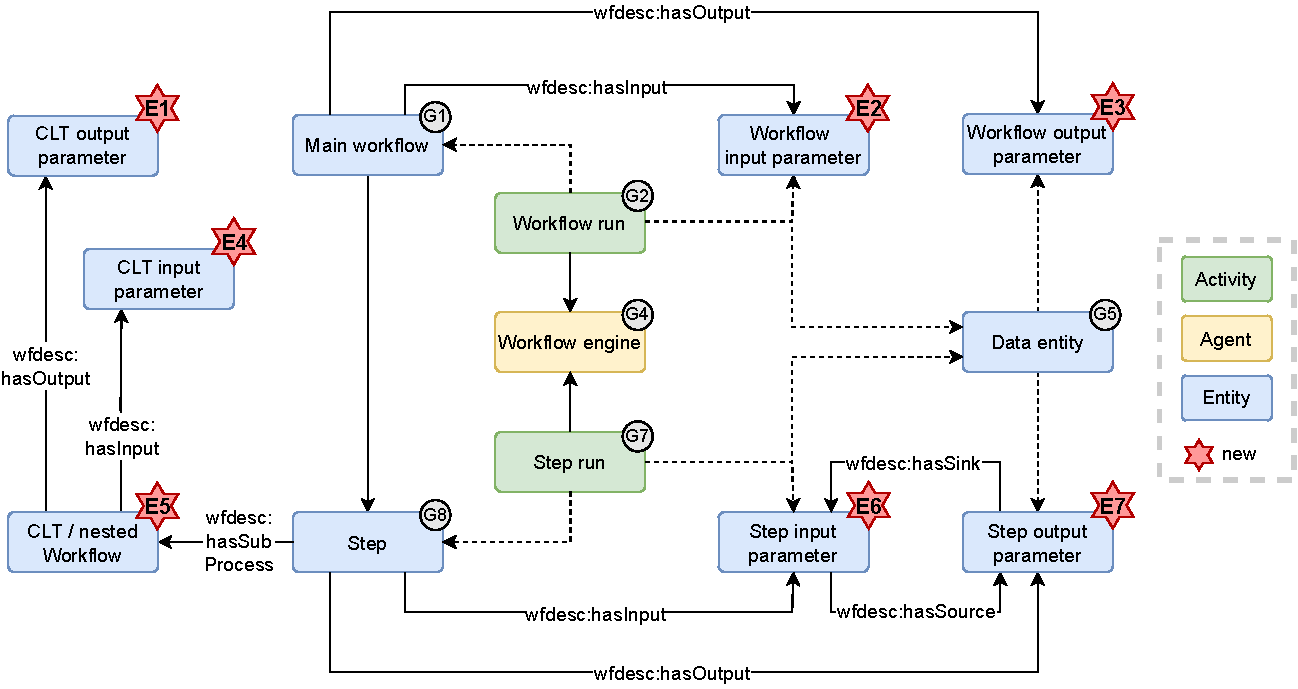
\includegraphics[width=0.99\textwidth]{rdf_extension/CWLProv_graph_extended.pdf}
    \caption{The RDF provenance graph, now extended with \emph{CommandLineTools} and parameter entities. Red stars mark nodes which are part of the design extension. Parameters are linked to their \emph{Workflow}, \emph{CommandLineTool} or step via \emph{wfdesc:hasInput} and \emph{wfdesc:hasOutput}. Node G5 represents both input and output data entities. The data flow between steps is represented via \emph{wfdesc:hasSink} and \emph{wfdesc:hasSource}. Steps are linked to their underlying tools via \emph{wfdesc:hasSubProcess}.}
    \label{fig:cwlprov_graph_new}
\end{figure*}



\begin{figure}[ht]
    \centering
    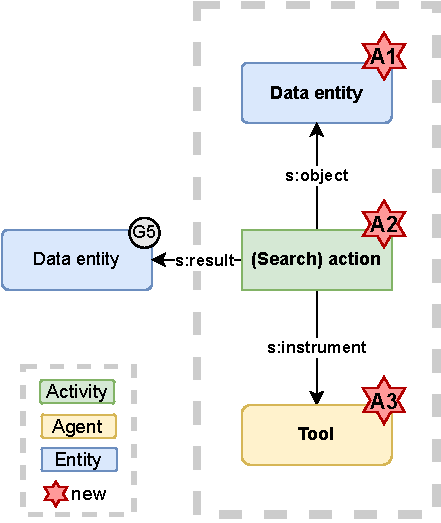
\includegraphics[width=0.4\textwidth]{rdf_extension/CWLProv_graph_extended_actions.pdf}
    \caption{Actions represented in RDF provenance graph. Workflow input datasets (\textbf{G5}) are connected to the Actions (\textbf{A2}) which produced them via \emph{s:result}. In addition, Actions can have properties such as \emph{object} (\textbf{A1}) and \emph{instrument} (\textbf{A3}).  }
    \label{fig:cwlprov_graph_actions}
\end{figure}

In Section \emph{\nameref{sec:cwlprov_evaluation}}, we analyzed CWLProv for the representation of the provenance taxonomy we defined in \emph{\nameref{sec:user_req}}. Based on this analysis, we concluded that not all provenance components were sufficiently represented in a structured format. Specifically, we found that although certain metadata was part of \emph{primary-job.json} and \emph{packed.cwl}, these annotations were not represented in RDF format.

In this section, we propose an extension of the design of the CWLProv provenance graph, which can at least represent the values for already supported metadata fields and can also be extended later with other metadata. %In this way, we (partially) answer \ref{rq:improve}.

Here, we are only concerned with the representation of this information, if it exists. Mechanisms for the collection of the metadata (whether it be manually or automated), are considered out of scope for this paper. 

In Section \emph{\nameref{sec:ext_reqs}}, we first describe the requirements and principles which we used in this design. Subsequently, in Section \emph{\nameref{sec:ext_overview}}, we give a high-level overview of the design. We then give recommendations for specific terms and vocabulary which can be used for the metadata fields \emph{doc}, \emph{label}, \emph{intent}, and \emph{format} which are part of v1.2 of the CWL Standards (Section \emph{\nameref{sec:ext_details}}). We describe how we have partially realized this design in \emph{cwltool} (Section \emph{\nameref{sec:realization}}). Finally, we provide a list of SPARQL queries in Section \emph{\nameref{sup:sparql}}.
\stodor{keep the analysis in?}

\subsection{Requirements and principles}
\label{sec:ext_reqs}
For this design, we reuse principles \ref{pr:bioschemas} and \ref{pr:current_standards}. In addition, the RDF extension should adhere to four requirements.

\begin{enumerate}[label=\textbf{PR\arabic*}]
    \item \label{pr:metadata_fields} Represent the annotations that are supported in CWL workflows according to the CWL standards v1.2, summarized in Table \ref{tab:metadata_fields}.
    \item \label{pr:input} Represent the annotations for \emph{Files} and \emph{Directories} proposed in Section \emph{\nameref{sec:annot_cwl_now}}.
    \item \label{pr:execution} Represent the annotations for a collection of input values proposed in Section \emph{\nameref{sec:annot_cwl_now}}.
    \item \label{pr:actions} Represent the annotations for Actions proposed in Section \emph{\nameref{sec:annot_new_cwl}}.
\end{enumerate}

\subsection{High-level overview}
\label{sec:ext_overview}
In this section, we present a high-level overview of the extended provenance graph and link it to the requirements defined in Section \emph{\nameref{sec:ext_reqs}}.

\subsubsection{Representation of CWL metadata fields}

\begin{table}[bt!]
\caption{Metadata fields in CWL Standards v1.2. \emph{format} is only allowed for parameters of type File or File array.}\label{tab:metadata_fields}
\begin{tabularx}{\linewidth}{L l l l l}
\toprule
Workflow component & label & doc & intent & format \\
\midrule
% Widgets & 42 & Over-supplied\textsuperscript{*} \\
% Gadgets & 13 & Under-supplied \\
Workflow & \textbullet & \textbullet & \textbullet & ~\\ %\hline
WorkflowStep & \textbullet & \textbullet & ~ & ~\\ %\hline
CommandLineTool & \textbullet & \textbullet & \textbullet & ~\\ %\hline
ExpressionTool & ~ & ~ & \textbullet & ~\\ %\hline
WorkflowInputParameter & \textbullet & \textbullet & ~ & \textbullet\\ %\hline
WorkflowOutputParameter & \textbullet & \textbullet & ~ & \textbullet\\ %\hline
WorkflowStepInput & \textbullet & ~ & ~ & ~\\ %\hline
WorkflowStepOutput & ~ & ~ & ~ & ~\\ %\hline
CommandInputParameter & \textbullet & \textbullet & ~ & \textbullet\\ %\hline
CommandOutputParameter & \textbullet & \textbullet & ~ & \textbullet\\ %\hline
\bottomrule
\end{tabularx}
\end{table}

Figure \ref{fig:cwlprov_graph_new} shows how we extended the provenance graph to represent all current metadata fields (\ref{pr:metadata_fields}). \textbf{In the new graph, every workflow component in Table \ref{tab:metadata_fields} is represented as a distinct entity, and interrelated with terms from the \emph{wfdesc} ontology (\ref{pr:bioschemas}).} 
We added entities describing the CWL tools that are run by the steps (\textbf{E5}) and linked them to their input (\textbf{E4}) and output parameters (\textbf{E1}) via \emph{wfdesc:hasInput} and \emph{wfdesc:hasOutput}. We connected the steps (\textbf{G8}) and tools via \emph{wfdesc:hasSubProcess}. In addition, we linked the step parameters (\textbf{E6}, \textbf{E7}) together via \emph{wfdesc:hasSource} and \emph{wfdesc:hasSink} to express the data flow between the steps.

In CWLProv 0.6.0, the execution of nested workflows is described in separate RDF documents. \textbf{Following the same strategy, we recommend to only represent top-level parameters of nested workflows in the primary provenance graph.} More detailed annotations can be represented in the separate RDF documents which describe the nested workflows.

\subsubsection{Representation of input data annotations}
This structure depicted in Figure \ref{fig:cwlprov_graph_new} also supports representation of the input data annotations described in \emph{\nameref{sec:annot_cwl_now}} (\ref{pr:input}), by transferring them to the data entities they describe (\textbf{G5}). 


\subsubsection{Representation of configuration settings annotations} Annotations describing a collection of parameters (\ref{pr:execution}) are specific to the workflow execution. Therefore, we recommend that these annotations are transferred to the entity in the provenance graph describing the workflow execution (\textbf{G2}).

\subsubsection{Representation of input data history}
In the annotation scheme described in Section \emph{\nameref{sec:annot_new_cwl}}, the history of (processed) input data is expressed through \emph{Actions}. Figure \ref{fig:cwlprov_graph_actions} presents their representation in RDF (\ref{pr:actions}). 
Actions (\textbf{A2}) are performed on objects, which are data entities not aggregated in the CWLProv RO (\textbf{A1}). Actions can have additional properties such as Tools (\textbf{A3}) or other annotations as summarized in Table \ref{tab:action_schemaorg}. They are connected to input data entities (\textbf{G5}) via \emph{s:result}. 



\subsection{Details of the design}
\label{sec:ext_details}
Here, we move from the structure of the provenance graph to the annotations that now can be attached to the newly added entities and with which terms they should be represented.

First, we describe which terms to use for the CWL-specific metadata fields \emph{doc}, \emph{label}, \emph{format}, and \emph{intent}.

Although we could use the exact terms with \emph{cwlprov} prefix, we aim for interoperability with other provenance representations, such as the RO-Crate specification. Therefore, we reuse Schema.org terms, and because this is in agreement with our annotation scheme:

\begin{itemize}
    \item \textbf{doc}: http://schema.org/description
    \item \textbf{label}: http://schema.org/name
    \item \textbf{format}: http://schema.org/encodingFormat
    \item \textbf{intent}: http://schema.org/featureList
\end{itemize}

\textbf{In addition, we recommend that custom annotations attached to workflow components and input objects are transferred as they are.} We make an exception for \emph{s:additionalType}, for which the value can be added to the \emph{types} of the entity it describes, instead of being literally transferred as \emph{s:additionalType}.

When entities are described with nested annotations (e.g. \emph{s:citation}), we recommend to make this a separate entity in the graph instead of a nested annotation, in compliance with the PROV data model (\ref{pr:bioschemas}).

\subsection{Partial realization in \emph{cwltool}}
\label{sec:realization}
\todorenske{Update, when this is published there should be full support in cwltool.}
Because of time constraints, we could only partially realize the provenance graph extension in \emph{cwltool}. At the time of writing, annotations directly associated with inputs of type \emph{File} and \emph{Directory}, as exemplified in \emph{\nameref{sec:annot_fair}}, are propagated to the RDF provenance record. However, annotations of the collection of input parameter values (\emph{\nameref{sec:annot_actions}}) or annotations under \emph{cwlprov:prov} (\emph{\nameref{sec:annot_new_cwl}}), are currently not represented in RDF.

\subsection{Conceptual analysis of the design extension}
\label{sec:ext_analysis}

\todorenske{leave in?}
To test the extended design, we analyzed the RDF provenance graph which would have been associated with the epitope prediction workflow we used as an example in this thesis. The elements of the design which were not yet realized in \emph{cwltool}, we emulated via manual annotations of the document. 

\subsubsection{SPARQL queries.}

\todorenske{replace with all sparql queries}
Here, we present two example SPARQL queries we issued on the emulated extended provenance graph. The first (\textbf{Q1}) extracts the DOIs of all publications which were the citations of the used inputs.

The second (\textbf{Q2}) lists the formats for every file for which this is specified.

\clearpage
% \section{Taxonomy}

\subsection{\ref{tax:context}: Definition of metadata for scientific context}
\label{sec:reasoning_reqs}

In ??, we presented scientific context (\ref{tax:context}) as one of the aspects that should be present in the collected provenance. In this section, we elaborate on what we mean with scientific reasoning and how it should be incorporated in provenance.

\textbf{Why:} Representing the scientific thinking process in provenance is meant to make the connection between the article advertising the research and the research itself, contained in the RO. This connection is bidirectional: ROs can be used as a guide during manuscript writing as well as for providing context for a third party who has read the paper and wants to understand the analysis in more depth.

\textbf{What:} The scientific context covers many aspects of the research, from the reasons why particular input data and parameter settings were chosen \cite{committeeonreproducibilityandreplicabilityinscienceReproducibilityReplicabilityScience2019}, to the design of the workflow (why particular steps were included), to the rationale for the study and the overall hypothesis of the research \cite{belhajjameResearchObjectSuite2014}\cite{grykWorkflowsProvenanceInformation2017}. Even negative results can be reported and explored strategies which did not work can be included \cite{stoddenEnhancingReproducibilityComputational2016}. In addition, it can include the interpretation of the results and their implications on the field (or maybe the output of an intermediate step warrants the inclusion of another preprocessing step).

\textbf{How:} We classify scientific context into 3 components:
\begin{enumerate}[label=\textbf{SC\arabic*}]
    \item \textbf{Workflow design}. Annotations on the design of the workflow and its components. Purpose of the workflow, why steps were included or excluded, the meaning of particular input parameters, etc. \label{req:sr_wf}
    \item \textbf{Entity annotations}: The meaning of individual input and output data entities. Why were they chosen? How are the results interpreted? \label{req:sr_data}
    \item \textbf{Workflow execution annotations}: Annotations about a set of parameters in a particular workflow run. Allows to distinguish between the ROs of multiple workflow runs. \label{req:sr_ex}
\end{enumerate}

% \subsection{\ref{tax:data}: Definition of metadata for data}
\label{sec:data_reqs}

In this section, we describe which metadata should be attached to data entities (\ref{tax:data}) in the provenance record. 

\textbf{What:} We mean not only input data, but also (intermediate) output data.

\textbf{Why:} Metadata associated with data entities can have at least two purposes:
\begin{itemize}
    \item \textbf{To explain the meaning and context of the data.} The context of the data should be described, because others need to be able to assess the appropriateness of the data for the purpose of the computational analysis. \textit{In the case of the epitope prediction workflow, it is important to understand the composition of the training set, since this is highly influential on the performance and applicability of the model.}
    \item \textbf{To describe data which is not contained in the RO.} To reduce RO size, or because the data cannot be shared for privacy reasons (it is proprietary or in other ways non-public), data may not be present in the RO but stored in an external repository. Characteristics of the data may still be included which provide information, to make sure that the data in the repository is the same as which was used in the original analysis. \textit{Use case \ref{uc:service} is an example where limiting the size of the RO may be desirable. Instead, the RO could contain references to datasets which are too large and are instead stored in an external repository.}
\end{itemize}

\textbf{How:} We identify 4 categories of data metadata which should be represented based on these two reasons. Here we link them to established recommendations and best practices for data citation, according to the FORCE11 Data Citation Principles \cite{datacitationsynthesisgroupJointDeclarationData2014}, which are based on the FAIR principles \cite{wilkinsonFAIRGuidingPrinciples2016}.

\begin{enumerate}[label=\textbf{D\arabic*}]
    \item \textbf{Identification}: PID, version, name and description of the dataset. Preferred citation of the data. \emph{When the data is not FAIR:} URL and download date as an alternative for PID and version. \emph{When the dataset is a subset of a larger collection (e.g. a database):} PID of database, database version and download date, and the query or filtering strategy which produced the dataset. \label{req:data_id}
    \item \textbf{File characteristics}: Filename, format, creation and last modification timestamps, size, and checksum. \label{req:data_char}
    \item \textbf{Access}: URL to a downloadable form of the data. License. \label{req:data_access}
    \item \label{req:data_mapping} \textbf{Mapping}: The workflow and step parameters for which the data is an input or output.
\end{enumerate}

% \subsection{\ref{tax:software}: Definition of metadata for software}
\label{sec:software_reqs}

In this section, we elaborate on the representation of software in the provenance record (\ref{tax:software}). 

\textbf{What:} In particular, we mean the command-line programs directly orchestrated by the workflow. However, these principles also apply to the workflow itself (\Cref{sec:wf_reqs}), the workflow engine (\Cref{sec:execution_reqs}), and computational environment (\Cref{sec:env_reqs}).

\textbf{Why:} There are two main reasons why software should be described with metadata:

\begin{itemize}
    \item \textbf{Obtaining identical results in a re-execution may be highly dependent on the version of the tools used.} This is important when reproducing the workflow. 
    \item \textbf{The original software may not be available or executable in the future.} In this case, the software should be sufficiently described for others to choose a suitable equivalent. 
\end{itemize}

\textbf{How}: We identify 3 categories of software characteristics which should be included in the provenance. Here we link them to established recommendations and best practices for software citation, according to the FORCE11 Software Citation Principles \cite{smithSoftwareCitationPrinciples2016}, which were adapted from the FORCE11 Data Citation Principles.

\begin{enumerate}[label=\textbf{SW\arabic*}]
    \item \textbf{Identification}: PID, name, version, release date and description of the software. Preferred citation. \textit{When the software is not FAIR:} URL of repository, download date and/or git commit hash as substitute for PID, version or release date. \label{req:sw_id}
    \item \textbf{Documentation}: URL of documentation or other metadata which is important to make informed use of the tool. URL to repository with source code of the software. \label{req:sw_doc}
    \item \textbf{Access}: URL to downloadable, executable form of the software. License. \label{req:sw_access}
\end{enumerate}


% \subsection{\ref{tax:wf}: Definition of metadata for workflow}
\label{sec:wf_reqs}

In this section, we describe the metadata that is associated with the workflow (\ref{tax:wf}). 

\textbf{What}: We define workflow here as the documents described in CWL (for other workflows, this would be the top-level script, not the underlying software that it controls). Hence the workflow comprises the main workflow description and the \emph{CommandLineTool} and nested \emph{Workflow} descriptions. 

\textbf{Why}: Workflows provide both a high-level overview of the analysis as well as details which are difficult to convey in a textual format in the Methods section of a scientific article \cite{gilAutomatingDataNarratives2017}. In addition, workflows are software which should be preserved and reused \cite{gobleFAIRComputationalWorkflows2020}. 

\textbf{How}: The metadata associated with workflows comprise general software metadata, in addition to workflow-specific information. 
\begin{enumerate}[label=\textbf{WF\arabic*}]
\item \textbf{General software metadata}: At workflow and step level, according to \Cref{sec:software_reqs}. \label{req:wf_all}
\item \textbf{Parameters}: Type, format, and description, at workflow and step-level. \label{req:wf_param}
\item \textbf{Requirements}: Software and hardware resources which are required to execute the workflow or workflow steps. \label{req:wf_resources}
\end{enumerate}


% \subsection{\ref{tax:env}: Definition of metadata for computational environment}
\label{sec:env_reqs}

In this section, we describe the requirements for computational environment (\ref{tax:env}).

\textbf{What}: Environment encompasses both software and hardware infrastructure, and may be part of a software container.

\textbf{Why}: Information about the computational environment is important for reproducing the workflow (\ref{uc:reproducing}). 

\begin{itemize}
    \item \textbf{Required resources:} Details about the resources available on the system which executed the original analysis can give an indication of what is necessary to rerun the workflow, even if this is not documented in the workflow description.
    \item \textbf{Debugging:} The generated output (or executability) of a step may be sensitive to specific versions of the tool orchestrated by the step or its dependencies.
\end{itemize}

\textbf{How}: We discriminate between three components of the computational environment:
\begin{enumerate}[label=\textbf{ENV\arabic*}]
    \item \textbf{Software}: software (dependencies), operating system. Dependencies could comprise all installed software (might contain much redundant information if a step was not executed in a software container), or the dependencies of the software which is run (which may be difficult to identify). Should follow the requirements as described in \Cref{sec:software_reqs}. \label{req:env_software}
    \item \textbf{Hardware}: Available RAM, storage, number and type of CPUs and GPUs. Network access. \label{req:env_hardware}
    \item \textbf{Container image}: Image name, tag and digest (because names and tags are not stable). Additional metadata (extracted from image labels), contents of Dockerfile (if built from Dockerfile), and general requirements for software as described in \Cref{sec:software_reqs}. \label{req:env_image}
\end{enumerate}

% \subsection{\ref{tax:execution}: Definition of metadata for execution details}
\label{sec:execution_reqs}

In this section, we define the final element of our provenance taxonomy: execution details (\ref{tax:execution}).

\textbf{What}: Executions are everything that is related to the analysis but which is not covered by the other categories. They constitute pure retrospective provenance: a record of what actually happened during the workflow run. 

\textbf{How}: We distinguish four components in this category:

\begin{enumerate}[label=\textbf{EX\arabic*}]
    \item \textbf{Timestamps}: When the workflow was executed, at step-granularity. The timestamps can be helpful when files were downloaded during the execution, especially from a database which does not have clear versions (SAbDab). In addition, the duration of the execution may be important during workflow development (test different settings) and when reproducing the workflow. \label{req:ex_time}
    \item \textbf{Consumed resources}: The resources used during execution, at step-granularity. This is different from what was described in \Cref{sec:env_reqs}, because there we only described what was available, not what was actually used. \label{req:ex_resources}
    \item \textbf{Workflow engine}: Software, therefore with same metadata as general software entities (\Cref{sec:software_reqs}).\label{req:ex_engine}
    \item \textbf{Human agent}: At a minimum, a PID such as ORCID should be included, or name and email of the person who ran the workflow. These details may be important for attribution (\ref{uc:writing}), and can also be used by third parties to ask further questions about the research.  \label{req:ex_human}
\end{enumerate}


\onecolumn
\section{SPARQL queries}
\label{sup:sparql}

\subsection{How to run the queries}

\begin{verbatim}
import rdflib
from rdflib.plugins.sparql import prepareQuery
from rdflib.namespace import Namespace
import pandas as pd

def run_query(rdf_file, query_file, namespaces):
    """
    rdf_file = RDF file; query_file = path to sparql query file; namespaces = Namespace object for every prefix in the SPARQL query.
    """
    g = rdflib.Graph()
    g.parse(rdf_file)
    with open(query_file, 'r')  as f:
        query_string = f.read()
        query = prepareQuery(
            queryString = query_string,
            initNs = namespaces,
        )

    print(f"SPARQL QUERY IS:\n{query}")
    
    qres = g.query(query)
    
    results = pd.DataFrame(qres.bindings).map(str).rename(columns=str)
    return results

def extract_wf_namespace(rdf_file):
    """
    Function which extracts namespace from CWLProv RDF provenance graph.
    """
    g = rdflib.Graph()
    g.parse(rdf_file)
    namespaces = list(g.namespaces())
    wf_namespace = ""
    for ns in namespaces:
        (prefix, namespace) = ns
        if prefix == "wf":
            wf_namespace = namespace

    return wf_namespace

provenance_file = "/path/to/provenance/file.ttl"
query_file = "/path/to/sparql/query/file.sparql" # file with any of the SPARQL queries listed in the section below

SCHEMA = Namespace("http://schema.org/")
WFDESC = Namespace("http://purl.org/wf4ever/wfdesc#")
wf_namespace = extract_wf_namespace(provenance_file)

namespaces = {"wf": wf_namespace, 
              "wfdesc": WFDESC,
              "schema": SCHEMA }

# How to run the query
response = run_query(provenance_file, query_file, namespaces)
\end{verbatim}

\subsection{SPARQL queries}

\noindent
\textbf{Return the \emph{doc}, \emph{label} and \emph{intent} fields of the main workflow.}

\lstinputlisting[basicstyle=\footnotesize]{sparql_queries/queries/wf_metadata_fields.sparql}

\noindent
\textbf{List \emph{doc} and \emph{label} fields of all \emph{WorkflowSteps} in the main workflow.}


\lstinputlisting[basicstyle=\footnotesize]{sparql_queries/queries/wf_step_metadata_fields.sparql}

\noindent
\textbf{Return the \emph{doc}, \emph{label} and \emph{intent} fields of every command-line tool or nested workflow that is run by each of the steps.}

\lstinputlisting[basicstyle=\footnotesize]{sparql_queries/queries/clt_nested_wf_metadata_fields.sparql}

\noindent
\textbf{List \emph{doc}, \emph{label}, \emph{format} fields of all input parameters of main workflow.}

\lstinputlisting[basicstyle=\footnotesize]{sparql_queries/queries/wf_input_params_metadata_fields.sparql}

\noindent
\textbf{List \emph{doc}, \emph{label}, \emph{format} fields of all output parameters of main workflow.}

\lstinputlisting[basicstyle=\footnotesize]{sparql_queries/queries/wf_output_params_metadata_fields.sparql}

\noindent
\textbf{List \emph{doc}, \emph{label}, \emph{format} fields of all input parameters of nested \emph{Workflows}/\emph{CommandLineTools}.}

\lstinputlisting[basicstyle=\footnotesize]{sparql_queries/queries/clt_nested_wf_input_params_metadata_fields.sparql}

\noindent
\textbf{List \emph{doc}, \emph{label}, \emph{format} fields of all output parameters of nested \emph{Workflows}/\emph{CommandLineTools}.}


\lstinputlisting[basicstyle=\footnotesize]{sparql_queries/queries/clt_nested_wf_output_params_metadata_fields.sparql}

% \clearpage

\section{SUPPLEMENTARY}

\stodor{Replaces \textbf{Methods} section. \url{https://academic.oup.com/gigascience//pages/research}}

\section{Use case workflow}
\label{sup:workflow}
\todorenske{Text in supplementary is for a large part identical to the thesis, not paraphrased}
% \todorenske{Change `epitope' to `PPI'? Extra explanation that we adapted the PPI model to epitope prediction?}

In this section, we describe the design and implementation of our exemplary bioinformatics workflow. First, we formulate the requirements which our workflow design should fulfill. Subsequently, we provide a detailed description of our CWL implementation of the design.

\subsection{Requirements}
\label{sec:wf_requirements}


The CWL implementation of our example workflow should meet two requirements, which we explain further in the subsequent sections:

\begin{enumerate}[label=\textbf{WR\arabic*}]
    \item \label{wr:method} Adhere to a specific method of epitope prediction which was conceptualized and provided to us by the workflow authors.
    \item \label{wr:reproducibility} Address challenges which compromise the transparency and reproducibility of the workflow.
\end{enumerate}


\subsection{\ref{wr:method}: Adhere to a conceptual method}
\label{sec:wf_design}

In this section, we explain \ref{wr:method}, providing a conceptual overview of the method which should be implemented in the CWL workflow we used as an exemplary workflow in this work.

The design of the epitope predictor, conceptualized by the workflow authors, is based on a model for predicting `general' protein-protein interaction (PPI) interfaces \cite{capelMultitaskLearningLeverage2022}. In its turn, that model was derived from OPUS-TASS \cite{xuOPUSTASSProteinBackbone2020}, a predictor for protein \emph{structure}. 

It addresses the lack of training data via a multi-task learning strategy, in which the model not only learns the label of interest (epitopes), but also related characteristics, such as solvent accessibility (the fraction of amino acid surface which is exposed to the aqueous environment). This allows the model to be trained on a larger set of structures, not restricted to antibody-antigen complexes, but also including structures with general PPI interfaces and other structural information.

The PPI predictor on which this method was based, was trained on OPUS-TASS reference data and did not include calculation of the input features or labels. In contrast, the OPUS-TASS source code did contain calculation of the input features, but the labels were reused from a reference dataset and not directly derived from protein structure. \textbf{However, because we wanted to maximize the transparency of our research, our workflow comprises the entire trajectory from protein structure and sequence to labels and features used for model training.} 

\subsubsection{Data sources}
These are the (main) data sources used to calculate the input features and labels:

\begin{itemize}
    \item \textbf{Protein Data Bank (PDB)} \cite{bermanProteinDataBank2000}, a database of experimentally resolved structures of proteins and complexes.
    \item \textbf{Structural Antibody Database (SAbDab)} \cite{dunbarSAbDabStructuralAntibody2014},  a database of metadata for antibody-antigen complexes in the PDB (e.g., which part of the complex corresponds to the antibody and which to the antigen).
    \item \textbf{BioDL} \cite{stringerPIPENNProteinInterface2022}, a dataset of protein sequences containing annotations for general PPI interactions, previously derived from structure.
    \item \textbf{HHBlits reference database.} Used by HHBlits \cite{remmertHHblitsLightningfastIterative2012} to compute some of the input features.
\end{itemize}

\subsubsection{Structure-derived labels}
For each residue in each protein sequence, the model predicts a number of properties. 

\begin{itemize}
    \item \textbf{Epitope}: a binary label indicating if a given residue is an epitope. Calculated from protein structure in combination with SAbDab metadata. Missing for proteins which are not included in SAbDab.
    \item \textbf{PPI}: a binary label indicating if a given residue is part of a general PPI interface. Extracted from BioDL.
    \item \textbf{Surface accessibility}: a label indicating how much of the amino acid is exposed to the surface. Calculated by DSSP \cite{kabschDictionaryProteinSecondary1983} based on the protein structure.
    \item \textbf{Secondary structure}: 3 binary labels indicating the secondary structure of which a given residue is part (alpha helix, beta strand or loop). Calculated by DSSP based on the protein structure. 
\end{itemize}

\subsubsection{Sequence-derived input features}
The model predicts epitope annotations based on three groups of sequence-derived features:
\begin{itemize}
    \item \textbf{PC7}: 7 features which reflect amino-acid-specific physico-chemical characteristics. Every amino acid type has fixed values for these features.
    \item \textbf{PSP19}: 19 binary features which reflect the presence of particular amino acid `building blocks' (e.g. a benzene ring). Every amino acid type has fixed values for these features.
    \item \textbf{HHM}: 30 features derived from a sequence profile generated from alignment with highly similar sequences. Computed with HHBlits.
\end{itemize}

\subsection{\ref{wr:reproducibility}: Address reproducibility challenges for this workflow}
\label{sec:wf_reproducibility}

In this section, we explain \ref{wr:reproducibility} by presenting a number of characteristics of our workflow which may make its implementation challenging from a transparency and reproducibility perspective.

\subsubsection{Workflow design}

Firstly, the method requires calculation of over 50 input features and at least 6 labels for every amino acid in each of the several thousand proteins in the training dataset, involving three data sources, at least two command-line tools and several Python scripts. This underlines the importance of describing this process as a workflow, in order to keep track of all the data flows. 

Secondly, the design of the workflow is subject to extensive changes, as the workflow authors test different combinations of input features and labels in order to optimize performance as well as computational efficiency. In addition, they may need to include extra preprocessing steps to remove potential bias from the training set (e.g. due to overrepresentation of certain protein families in the PDB).

\subsubsection{Software}

The workflow steps each have their respective software dependencies, some of which are only compatible with particular versions of other software (e.g. \emph{tensorflow}). Recording the versions of tools and dependencies is therefore very important for reproducibility.

\subsubsection{Data}
Retrieving and handling the data used as input for this workflow has its own challenges. 
Firstly, HHBlits can be used with different reference databases, which will influence the produced sequence profiles. These databases have versions, and are not stored in a FAIR manner. 

Secondly, the dataset downloaded from PDB does not comprise the entire database, but a subset which is selected as the result of a query. Since new entries are added to PDB continually, it is not likely that running the same query at a later moment will result in the same dataset. Similarly, SAbDab also receives weekly updates \cite{dunbarSAbDabStructuralAntibody2014}. 

Finally, the identifiers in the BioDL dataset correspond to particular \emph{sequences}, whereas those in SAbDab and PDB represent \emph{structures}. Therefore, we need to match the two types of identifiers with each other. However, external resources such as the UniProt mapping tool\footnote{\url{https://www.uniprot.org/id-mapping/}} \cite{theuniprotconsortiumUniProtUniversalProtein2021} may not return the same mappings in the future.

\subsection{CWL implementation of the workflow}
\label{sec:wf_implementation}

In this section, we describe how we implemented the epitope prediction workflow in CWL, considering the requirements described in the previous sections. Figure \ref{fig:wf} shows an overview of the CWL implementation of the workflow.

\subsubsection{Implementation of the conceptual method (\ref{wr:method})}

To address the first requirement, the workflow starts by issuing a query to the PDB Search API\footnote{\url{https://search.rcsb.org/index.html\#search-api}} (\emph{run\_pdb\_query}). This produces a list of PDB IDs which is used to download the protein structures from PDB (\emph{download\_pdb\_files}), which are subsequently decompressed (\emph{decompress\_pdb\_files}). From the protein structures, DSSP calculates surface accessibility and secondary structure (\emph{generate\_dssp\_labels}), and an in-house Python script extracts epitope annotations (\emph{generate\_epitope\_labels}) using a SAbDab summary file which has been preprocessed in an earlier step (\emph{preprocess\_sabdab\_data}). Another Python script extracts PPI annotations from BioDL and performs identifier mapping (\emph{generate\_ppi\_labels}). Three separate steps calculate input features for the protein sequences with PPI annotations (\emph{generate\_hhm}, \emph{generate\_pc7}, and \emph{generate\_psp19}). The input features and labels are subsequently combined in two steps  (\emph{combine\_features}, \emph{combine\_labels}) and used to train the prediction model (\emph{train\_epitope\_prediction\_model}).

\subsubsection{Consideration of workflow reproducibility  (\ref{wr:reproducibility})} 
Firstly, we aimed to automate the workflow as much as possible. For this reason, the PDB query and download steps are included in the workflow (with the query as one of the workflow inputs). The two workflow inputs constituting the BioDL dataset (\emph{biodl\_test\_dataset} and \emph{biodl\_train\_dataset}) are included as remote files and downloaded by \emph{cwltool} during workflow execution. 
Because SAbDab is not programmatically accessible, \emph{sabdab\_summary\_file} needs to be downloaded manually, but all further preprocessing steps are included of the workflow. 

To avoid using external mapping tools between UniProt and PDB identifiers, we infer the relationships between the two types of IDs from the downloaded PDB files, which contain both types of identifiers. 

To make the workflow design easy to adapt and modify with different combinations of input features and labels, we spread the computation of these features over separate steps. This is different from the original OPUS-TASS code, in which all input features are calculated by a single Python script. 

To increase the portability of the computational environment, some steps are executed inside software containers. The workflow engine pulls Docker images from external repositories and converts them to Singularity \cite{kurtzerSingularityScientificContainers2017} containers, the software which is installed on the Bazis HPC cluster on which we executed the workflow. 
% Steps for which there was no image available can be containerized in the future by building custom images from Dockerfiles and uploading them to our own repository.

\subsubsection{Emulation of workflow steps} 
Because this workflow is still in development, some steps are emulated. In this way, the steps produce output in the expected format, but do not necessarily contain biologically sensible information. 

In summary, for three steps we used scripts provided by the workflow authors (\emph{preprocess\_sabdab\_data}, \emph{generate\_epitope\_labels}, and \emph{generate\_dssp\_labels}). For other steps we reused or modified code from OPUS-TASS (\emph{generate\_pc7}, \emph{generate\_psp19}, and \emph{generate\_hhm}) or other sources (\emph{run\_pdb\_query}, \emph{download\_pdb\_files}). Finally, we wrote custom Python scripts for the remaining steps, of which two were partially (\emph{combine\_labels}) or completely emulated (\emph{train\_epitope\_prediction\_model}). 

\clearpage
\section{Provenance questions}\label{sup:provquestions}

% \todorenske{How to organize this section? Idea 1: leave it as it is. Idea 2: Make sideways table with 1 question per row, add columns for each use case (U1 - U5) and provenance subcomponent (SC1, SC2, SC3, D1, ...). Indicate for which use case and provenance component each question is applicable. }

\newlist{provquestions}{enumerate}{1}
\setlist[provquestions, 1]
{label=Q\arabic{provquestionsi}., %1., 2., 3., ...
leftmargin=2\parindent,
rightmargin=10pt
}


\subsection*{\ref{uc:wf_dev}: Workflow development}

\begin{provquestions}
    \item What is the influence of including filtering step X on performance? (SC1, SC2, EX1)
    \item What is the influence of a different model architecture on performance? (SC1, SC2, EX1)
    \item What is the influence of a different training set on performance? (SC2, EX1)
    \item What is the influence of a different value for input parameter X on performance? (SC2, EX1)
    \item What is the influence of removing model training feature X on performance? (SC2, EX1)
    \item What is the difference between workflow runs X and Y? (SC3)
    \item Which of workflow runs X and Y used more RAM? (SC3, EX2)
    \item Under which conditions am I allowed to reuse this third-party dataset as input for my workflow? (D3)
    \item Under which conditions am I allowed to reuse this third-party software tool for my workflow? (SW3)
    \item What is the influence of ... on training time? (EX1)
\end{provquestions}

\subsection{\ref{uc:writing}: Publishing the workflow}
\begin{provquestions}[resume]
    \item On which previous research was this research built (conceptually)? (SC1)
    \item Which of my colleagues contributed to the conceptualization of this research? What were their contributions? (SC1, WF1, EX4)
    \item Which cleaning operations were performed on workflow input X? (SC2, D1)
    \item Which were all the datasets I used as inputs and should be cited? (D1)
    \item When was dataset X downloaded from database Y? (D1, D2)
    \item What are all the resources which contributed to this research (and should be cited)? (D1, SW1)
    \item Which software was used in this workflow? (SW1)
    \item I reused a custom, unpublished script made by one of my collaborators. How do I give credit to the original authors? (SW1)
    \item I wrote a custom script based on existing code. How do I give credit to the original authors? (SW1)
    \item I wrote a CWL \emph{CommandLineTool} description for existing software. How do I cite it? (SW1)
    \item I reused an existing CWL CommandLineTool description. How do I give credit to the original authors? (WF1)
    \item Which of my colleagues contributed to this workflow to whom I should give credit and/or propose as co-authors? What were their contributions? (WF1)
    \item From which workflow(s) was this workflow derived? (WF1)
    \item I reused a Dockerfile or Docker container image which was written or built by someone else. How do I give credit to the original authors? (ENV3)
\end{provquestions}

\subsection{\ref{uc:understanding}: Understanding the workflow}
\begin{provquestions}[resume]
    \item What is the goal of this analysis? (SC1)  
    \item Why was this step included? (SC1)
    \item Why was this combination of steps chosen? (SC1)
    \item What is the interpretation of this (intermediate) output?  (SC2)
    \item What was the performance of the model? (SC2)
    \item What was the hypothesis of this workflow run? (SC3)
    \item Why was this set of values chosen as inputs for this workflow execution? (SC3)
    \item Where can I find more information about BioDL dataset? (D1)
    \item Which SAbDab query was used to generate the summary file? (D1)
    \item Which UniProt IDs are part of BioDL? (D1)
    \item Which query was issued to PDB? (D1)
    \item How was this figure from the paper generated? (D1)
    \item For which workflow parameter is this dataset an input? (D4)
    \item Which workflow step produced this output file? (D4)
    \item What was the model architecture? (SW2)
    \item Which related tasks were predicted by the model? (SW2)
    \item How were UniProt IDs mapped to PDB IDs? (WF1)
    \item Which input features were used for the model? (WF2)
    \item What are the values of PSP19 for each amino acid type? (WF2)
    \item What is the format of this output file? (WF2)
    \item How should I cite \emph{cwltool}? (EX3)
    \item Who can I contact for more information about the research? (EX4)
\end{provquestions}

\subsection{\ref{uc:reproducing}: Reproducing the workflow}

\begin{provquestions}[resume]
    \item Which HHBlits reference database was used? Which version? (D1)
    \item What was the last modification date of this input file? (D2)
    \item Where can I download HHBlits reference database? (It was not stored in the RO because of its large size.) (D3)
    \item Which version of HHBlits was used? (SW1)
    \item The CWL \emph{CommandLineTool} description did not describe all parameters of this command-line program. Which values were used for the other parameters? (SW2)
    \item Which format does the PDB batch download script need? (SW2)
    \item Where can I download HHBlits? (SW3)
    \item Does this step need network access? (WF3)
    \item How many CPUs are required for this step, according to the workflow description? (WF3)
    \item How much RAM is necessary for this step, according to the workflow description? (WF3)
    \item Which software (and their versions) was installed on the system? (ENV1) 
    \item Which CPU/GPU was installed? (ENV2)
    \item Original author used Dockerfile. Is the image I built on a rerun the same as the one in the original analysis?  (ENV3)
    \item I pulled a Docker image. Is this the same as which was used in the original analysis? (ENV3)
    \item How long does this step take? (EX1)
    \item When was PDB database queried? (EX1)
    \item When was SAbDab database queried? (EX1)
    \item How much memory was used in the original run? (EX2)
    \item Which version of \emph{cwltool} was used in the original run? (EX3)
    \item Who ran the original workflow and how can I contact them for more information? (EX4)
\end{provquestions}

\subsection{\ref{uc:service}: Model as a web service}

\begin{provquestions}[resume]
    \item What was the query which returned the set of proteins for which I made predictions with the model? (SC2, D1)
    \item Which protein sequences were in the training set? (SC2, D1)
    \item Which proteins had epitope annotations? (SC2, D1)
    \item How should I cite this tool? (WF1)
\end{provquestions}

\clearpage
\section{Annotation scheme}
\label{sup:annotation}


\subsection{Requirements} \label{sec:annot_req}

Based on the results of the analysis described in Section \emph{\nameref{sec:cwlprov_evaluation}}, the input annotation scheme should meet the following requirements:

\begin{enumerate}[label=\textbf{IR\arabic*}]
    \item \label{ir:metadata} Represent the elements defined in \textbf{D1} and \textbf{D3}.
    \item \label{ir:types} Describe input data of type \emph{File}, \emph{Directory} and \emph{Array}.
    \item \label{ir:history} Represent the history of processed input data (e.g filtering).
    \item \label{ir:query} Represent the database query which produced a dataset.
    \item \label{ir:extend} Support extension with domain-specific vocabularies.
    \item \label{ir:context} Represent information about a set of input parameters (\textbf{SC3})
\end{enumerate}

\subsection{Design principles}
\label{sec:annot_principles}

The design of the input data annotation scheme was based on a set of underlying principles:

\begin{enumerate}[label=\textbf{IP\arabic*}]
    \item \textbf{Reuse of existing terms and ontologies.} Our scheme uses Schema.org, since this complies with the Bioschemas \cite{grayPotatoSaladProtein2017} initiative. Schema.org terms are also adopted by related efforts such as the RO-Crate specification \cite{soiland-reyesPackagingResearchArtefacts2022}. \label{pr:bioschemas}
    \item \textbf{Extension of the CWL standards only when absolutely necessary.} We started from the latest CWL Standards specification (v1.2), and only where these did not support adding metadata we proposed an extension. \label{pr:current_standards}
    \item \textbf{Clear separation between input data and metadata.} This keeps the input object document relatively easy to understand. \label{pr:separate}
    \item \textbf{Simplicity.} The annotation scheme should be easy to understand and use for CWL workflow authors. \label{pr:simplicity}
\end{enumerate}

\subsection{Annotations supported by CWL standards v1.2}
\label{sec:annot_cwl_now}
Here, we explain the annotations that are supported by the latest release of the CWL standards (\ref{pr:current_standards}). In the examples outlined below, we abbreviate \emph{\url{http://schema.org/}} with the prefix \emph{s:}.

\subsubsection{Format}
CWL Standards v1.2 support semantic annotations for \emph{File} and \emph{Directory} objects in the input object document. We recommend that annotations are appended on the same level as the standard fields (\emph{class}, \emph{location} and \emph{format}), where the property is the key and the annotation itself the value. Values can be single annotations, arrays or (arrays of) dictionaries. 

In addition, the authors can convey information about a \emph{set} of input parameters via annotations in the root of the input object document (\ref{ir:context}). 

\subsubsection{Vocabulary}
Information about a set of input values can be expressed under the \emph{s:description} key. 

For \emph{File} and \emph{Directory} inputs, we reused the Bioschemas Dataset profile v1.0\footnote{\url{https://bioschemas.org/profiles/Dataset/1.0-RELEASE}}, in this way complying with \ref{pr:bioschemas}. 
Table \ref{tab:dataset_bioschemas} shows how the Schema.org terms relate to the required metadata specified in \textbf{D1} and  \textbf{D3}. 

We recommend that authors adhere to this vocabulary when describing properties of their datasets which are domain-neutral. However, if they want to convey domain-specific information which is not covered by the terms in Table \ref{tab:dataset_bioschemas}, they may choose to extend this annotation scheme with domain-specific ontologies (such as EDAM \cite{isonEDAMOntologyBioinformatics2013}), in this way fulfilling \ref{ir:extend}. 

In Section \emph{\nameref{sec:sup_example_annotations}}, we show some annotation examples. In general, we recommend that authors provide at a minimum the metadata which is not covered by the identifier of the data they use (\ref{pr:simplicity}). 

\begin{table}[bt!]
\caption{Schema.org terms to use to express the metadata elements described in \ref{tax:data}. Taken from Bioschemas Dataset profile v1.0.}\label{tab:dataset_bioschemas}
\begin{tabularx}{\linewidth}{l l L}
\toprule
Schema.org & T2 element & Expected type \\
\midrule
        identifier & PID & URL \\ %\hline
        version & version & Number, Text \\ %\hline
        name & name & Text \\ %\hline
        description & description & Text \\ %\hline
        citation & citation & CreativeWork \\ %\hline
        includedInDataCatalog & database & DataCatalog \\ %\hline
        dateCreated & download date & Date, DateTime \\ %\hline
        dateModified & modification date & Date, DateTime \\ %\hline
        distribution & URL to data & DataDownload \\ %\hline
        license & license & URL \\ %\hline
\bottomrule
\end{tabularx}
\end{table}
\begin{table}[bt!]
\caption{Schema.org terms to represent the history of data inputs.}\label{tab:action_schemaorg}
\begin{tabularx}{\linewidth}{l l L}
\toprule
Schema.org & Expected type & Explanation \\
\midrule
% Widgets & 42 & Over-supplied\textsuperscript{*} \\
% Gadgets & 13 & Under-supplied \\
query & Text & Query used (only for SearchAction) \\ %\hline
object & Thing & Database or initial dataset \\ %\hline
result & Thing & Resulting dataset \\ %\hline
instrument & Thing & Tool used, e.g. for filtering \\ %\hline
endTime & DateTime, Time & Time of action \\ %\hline
agent & Organization, Person & Who performed the action \\ %\hline
description & Text & Description of the action \\ %\hline
\bottomrule
\end{tabularx}
\end{table}



\subsection{Proposed extension of CWL standards to support richer annotations.}
\label{sec:annot_new_cwl}

The previous section explained how the latest release of the CWL standards can support metadata annotations. However, with the presented annotation scheme, authors will find it difficult to explain the history of processed input data in a structured format (\ref{ir:history}). In addition, it is non-trivial to explain that a dataset (which can be a collection of files) is the result of a database query (\ref{ir:query}).

In this section, we propose an extension to the CWL standards which enables authors to annotate \emph{Arrays} (\ref{ir:types}), and represent queries and processing operations which lead to the dataset they used as input for the workflow execution.

\subsubsection{Format.} 

We propose that authors represent the history of their datasets as a sequence of actions in the input object document. These actions are performed on an initial dataset and produce a result. The result of an action can be the input of another.

To avoid obfuscating the input object document, the metadata must be listed under a \emph{cwlprov:prov} field, separate from the input values (\ref{pr:separate}). This is analogous to the \emph{overrides} field in the current CWL standards
\footnote{\RaggedRight\url{https://cwltool.readthedocs.io/en/latest/##overriding-workflow-requirements-at-load-time}}.% have to double the # to escape it

\subsubsection{Vocabulary.}

We used Schema.org terms to express search and processing actions. Table \ref{tab:action_schemaorg} lists the properties defined for \emph{s:Actions} and (more specific) \emph{s:SearchActions} and explains how they can be used in the annotation of CWL documents. In general, \emph{Actions} are performed on an \emph{object}, producing a \emph{result}. The action can be initiated by an \emph{agent}, using an \emph{instrument}. \emph{SearchActions} can be based on a \emph{query}. The moment the action was performed can be represented via \emph{endTime}.

\onecolumn
\subsection{Example input annotations}
\label{sec:sup_example_annotations}

\subsubsection{Annotations for a FAIR file.}
\label{sec:annot_fair}
The following is an example of a standalone dataset with its own identifier. In addition to the CWL-specific \emph{format} field (\emph{line 4}), we provided additional Schema.org terms in order to comply with \ref{ir:metadata}. In principle, providing the identifier and version with a description (\emph{lines 5-7}) is sufficient for unambiguous identification, since the identifier resolves to a landing page with additional information. However, for the purpose of our example, we added all other terms from Table \ref{tab:dataset_bioschemas} manually as well (\emph{lines 8-16}).

\begin{minted}[linenos,xleftmargin=\parindent, breaklines]{yaml}
FAIR_file:
  class: File
  location: path://path/to/6nzn.pdb
  format: http://edamontology.org/format_1476 # pdb
  s:identifier: https://doi.org/10.2210/pdb6nzn/pdb 
  s:version: "1.4"
  s:description: "Amyloid fibril structure of glucagon in pdb format."
  s:name: "6NZN"
  s:citation: 
    s:identifier: https://doi.org/10.1038/s41594-019-0238-6
  s:dateCreated: 2019-02-14
  s:dateModified: 2019-12-18 
  s:includedInDataCatalog: # PDB
    s:identifier: https://doi.org/10.25504/FAIRsharing.2t35ja
  s:distribution: https://ftp.wwpdb.org/pub/pdb/data/structures /divided/pdb/nz/pdb6nzn.ent.gz
  s:license: https://spdx.org/licenses/CC0-1.0
\end{minted}

\subsubsection{Annotations for a file without persistent identifier} \label{sec:annot_nonfair}
% \Cref{sup:annot_nonfair} 

When the dataset is not FAIR, the download or modification date (\emph{line 7}) can serve as an alternative for version. The URL of the remote file is used as an alternative to a persistent identifier (\emph{line 3}).

\begin{minted}[linenos,xleftmargin=\parindent, breaklines]{yaml}
nonFAIR_file:
  class: File
  location: https://www.ibi.vu.nl/downloads/PIPENN/PIPENN/BioDL-Datasets/prepared_biolip_win_p_testing.csv
  format: http://edamontology.org/format_3752 # csv
  s:additionalType: s:Dataset 
  s:name: "BioDL test set"
  s:dateModified: "2021-08-02" # an alternative to version
  s:citation:
    s:identifier: https://doi.org/10.1093/bioinformatics/btac071
  s:license: https://spdx.org/licenses/GPL-3.0-or-later.html
  s:description: "BioDL test set containing only protein-protein interactions."
\end{minted}


\subsubsection{Adding domain-specific annotations.}

The CWL standards also support adding domain-specific ontologies. Here we add extra information about the biological interpretation of the data, using terms from the EDAM ontology (with \emph{edam:} for  \emph{http://edamontology.org/}). In addition to the identifier, version and description (\emph{lines 5-7}), we explicitly define this file as a dataset and protein structure (\emph{lines 8-10}) and express the scientific domain to which it is related (\emph{line 11}). 

\begin{minted}[linenos,xleftmargin=\parindent, breaklines]{yaml}
domain_annotations_file:
  class: File
  location: path://path/to/6nzn.pdb
  format: http://edamontology.org/format_1476 # pdb
  s:identifier: https://doi.org/10.2210/pdb6nzn/pdb 
  s:version: "1.4"
  s:description: "Amyloid fibril structure of glucagon in pdb format."
  s:additionalType:
  - s:Dataset
  - edam:data_1460 # protein structure
  edam:has_topic: edam:topic_2814 # protein structure analysis
\end{minted}

\subsubsection{Annotation of a collection of input parameters.} \label{sec:annot_actions}
This example shows how scientific context can be represented, even for parameters which are not \emph{Files} or \emph{Directories}. Lines 1-5 denote the value of the workflow input parameters. The entire set of parameters is described via \emph{s:description} (\emph{line 7}), providing a mechanism to distinguish ROs of different workflow runs from each other.

\begin{minted}[linenos,xleftmargin=\parindent,breaklines]{yaml}
input1: "string value"
input2: 4
input3:
  class: File
  location: path://path/to/file.txt

s:description: "Workflow run without input feature X to test effect on model performance."
\end{minted}

\subsubsection{Example annotation of a sequence of actions.} 

In the following example, a database search was performed (\emph{lines 2-8}), followed by a filtering operation (\emph{lines 10-15}). The resulting dataset was used as an input for the workflow (\emph{lines 17-19}). Both actions are listed under \emph{cwlprov:prov} (\emph{line 1}). The result of the search action (\emph{line 7}) corresponds to the object of the filtering operation (\emph{line 12}). In this example, the query is provided in a human-readable format, but the exact query which was issued (a JSON string) could also be used.

\begin{minted}[linenos,xleftmargin=\parindent,breaklines]{yaml}
cwlprov:prov:
  pdb_search:
    s:additionalType: s:SearchAction
    s:query: "All proteins with at least 2 chains deposited between 2010 and 2022"
    s:object:
      s:identifier: https://bio.tools/pdb
    s:result: pdb_search_result
    s:endTime: 2022-08-01
      
  filtering_action:
    s:additionalType: s:Action
    s:object: pdb_search_result
    s:instrument: 
      s:identifier: https://bio.tools/pisces
    s:result: filtered_pdb_dataset

filtered_pdb_dataset:
  class: Directory
  location: path://path/to/directory/
\end{minted}

\subsubsection{Annotation of a merged dataset}

In this example, a dataset is constructed from two other datasets (\emph{lines 4-6}).
Here, the instrument is not a tool but a function (\emph{line 7})

\begin{minted}[linenos,xleftmargin=\parindent,breaklines]{yaml}
cwlprov:prov:
  merge_action:
    s:additionalType: s:Action
    s:object:
    - dataset1
    - dataset2
    s:instrument: pd.merge(dataset1, dataset2, on = "ID", how = "inner")
    s:result: merged_dataset
    s:description: "Imported both datasets as pandas dataframes, performed inner merge and saved as csv."

merged_dataset:
  class: File
  location: path://path/to/file.csv
\end{minted}

\subsubsection{Annotation of exemplary bioinformatics workflow}
Below, we show how we applied our annotation scheme to the input file for our example workflow. We represented the download action which produced the \emph{sabdab\_summary\_file} (\emph{lines 2-13}). If files were not downloaded during workflow execution, we supplied the URL to the dataset using \emph{s:distribution} (\emph{line 69}). Every file has a citation (\emph{s:citation}), consisting of the DOI of the primary publication. Finally, we supplied EDAM annotations to each \emph{File} and \emph{Directory} input (\emph{lines 29, 44, 58, 72}) and annotated the workflow run (\emph{line 78}). 
\begin{minted}[linenos,xleftmargin=\parindent,breaklines]{yaml}
cwlprov:prov:
  sabdab_search:
    s:additionalType: s:SearchAction
    s:query: "All structures"
    s:endTime: 2022-05-27
    s:object:
      s:additionalType: s:DataCatalog
      s:name: "Structural Antibody Database"
      s:citation:
        s:identifier: https://doi.org/10.1093/nar/gkab1050
    s:result: sabdab_summary_file
    s:description: "Search Action for metadata on antibody-antigen complexes in SAbDab"
    s:additionalType: edam:operation_0339 # structure database search

pdb_search_api_query:
  class: File
  location: path://path/to/pdb_query.json
  format: iana:application/json
  s:description: "Input query for PDB search API."
  s:additionalType:
  - edam:data_3786 # Query script

sabdab_summary_file:
  class: File
  path: path://path/to/sabdab_summary_all_20220527.tsv
  format: iana:text/tab-separated-values
  s:description: "Summary file downloaded from SAbDAb database, containing metadata for all structures."
  s:additionalType:
  - edam:data_2080 # database search results
  - s:Dataset
      
biodl_train_dataset:
  class: File
  location: https://www.ibi.vu.nl/downloads/PIPENN/PIPENN/BioDL-Datasets/prepared_biolip_win_p_training.csv
  format: http://edamontology.org/format_3752 # csv
  s:description: "BioDL training set containing PPI annotations for protein sequences (UniProt IDs)"
  s:name: "BioDL training dataset"
  s:dateModified: 2021-08-04
  s:citation:
    s:identifier: https://doi.org/10.1093/bioinformatics/btac071
  s:license: https://spdx.org/licenses/GPL-3.0-or-later.html
  s:additionalType:
  - s:Dataset
  - edam:data_1277 # protein features

biodl_test_dataset:
  class: File
  location: https://www.ibi.vu.nl/downloads/PIPENN/PIPENN/BioDL-Datasets/prepared_biolip_win_p_testing.csv
  format: http://edamontology.org/format_3752 # csv
  s:description: "BioDL test set containing PPI annotations for protein sequences (UniProt IDs)."
  s:name: "BioDL test dataset"
  s:dateModified: 2021-08-04
  s:citation:
    s:identifier: https://doi.org/10.1093/bioinformatics/btac071
  s:license: https://spdx.org/licenses/GPL-3.0-or-later.html
  s:additionalType:
  - s:Dataset
  - edam:data_1277 # protein features

hhblits_db_dir: 
  class: Directory
  location: path://path/to/uniclust30_2018_08/
  s:citation:
    s:identifier: https://doi.org/10.1038/nmeth.1818
  s:name: "uniclust30_2018_08_hhsuite"
  s:version: "2018_08"
  s:description: "Directory containing HHBlits reference database."
  s:license: https://spdx.org/licenses/CC-BY-SA-4.0
  s:distribution: https://wwwuser.gwdg.de/~compbiol/uniclust/2018_08/uniclust30_2018_08_hhsuite.tar.gz
  s:additionalType:
  - s:Dataset
  - edam:data_0955 # data index

hhblits_db_name: "uniclust30_2018"

hhblits_n_iterations: 1

s:description: "Demonstration run of epitope prediction workflow. Some steps are emulated, so the results of the workflow are not yet biologically meaningful."

$namespaces:
  iana: "https://www.iana.org/assignments/media-types/"
  s: "https://schema.org/"
  edam: "http://edamontology.org/"

$schemas:
- https://schema.org/version/latest/schemaorg-current-https.rdf
- https://edamontology.org/EDAM_1.25.owl
\end{minted}


\clearpage
\twocolumn
\section{Design of an extension of the CWLProv provenance graph}
\label{sec:dev_recommendatons}

\begin{figure*}[ht]
    \centering
    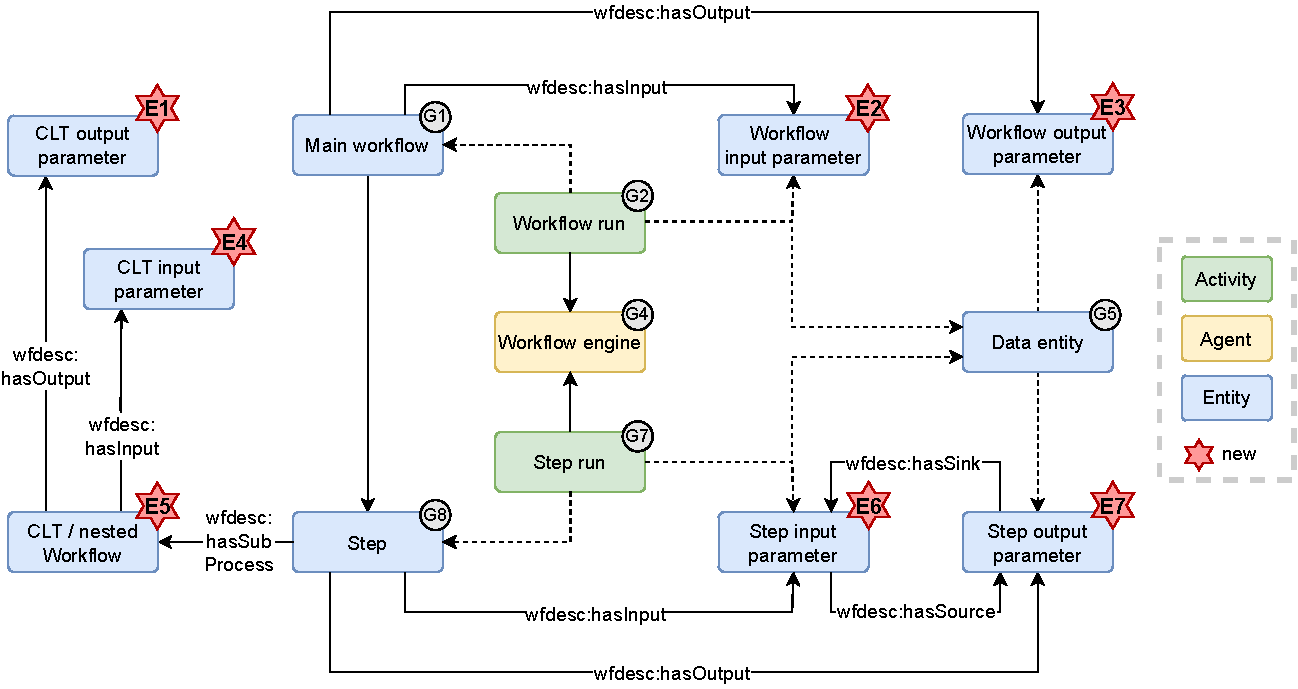
\includegraphics[width=0.99\textwidth]{rdf_extension/CWLProv_graph_extended.pdf}
    \caption{The RDF provenance graph, now extended with \emph{CommandLineTools} and parameter entities. Red stars mark nodes which are part of the design extension. Parameters are linked to their \emph{Workflow}, \emph{CommandLineTool} or step via \emph{wfdesc:hasInput} and \emph{wfdesc:hasOutput}. Node G5 represents both input and output data entities. The data flow between steps is represented via \emph{wfdesc:hasSink} and \emph{wfdesc:hasSource}. Steps are linked to their underlying tools via \emph{wfdesc:hasSubProcess}.}
    \label{fig:cwlprov_graph_new}
\end{figure*}



\begin{figure}[ht]
    \centering
    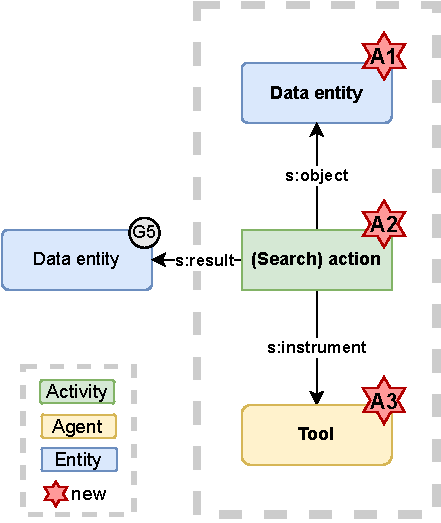
\includegraphics[width=0.4\textwidth]{rdf_extension/CWLProv_graph_extended_actions.pdf}
    \caption{Actions represented in RDF provenance graph. Workflow input datasets (\textbf{G5}) are connected to the Actions (\textbf{A2}) which produced them via \emph{s:result}. In addition, Actions can have properties such as \emph{object} (\textbf{A1}) and \emph{instrument} (\textbf{A3}).  }
    \label{fig:cwlprov_graph_actions}
\end{figure}

In Section \emph{\nameref{sec:cwlprov_evaluation}}, we analyzed CWLProv for the representation of the provenance taxonomy we defined in \emph{\nameref{sec:user_req}}. Based on this analysis, we concluded that not all provenance components were sufficiently represented in a structured format. Specifically, we found that although certain metadata was part of \emph{primary-job.json} and \emph{packed.cwl}, these annotations were not represented in RDF format.

In this section, we propose an extension of the design of the CWLProv provenance graph, which can at least represent the values for already supported metadata fields and can also be extended later with other metadata. %In this way, we (partially) answer \ref{rq:improve}.

Here, we are only concerned with the representation of this information, if it exists. Mechanisms for the collection of the metadata (whether it be manually or automated), are considered out of scope for this paper. 

In Section \emph{\nameref{sec:ext_reqs}}, we first describe the requirements and principles which we used in this design. Subsequently, in Section \emph{\nameref{sec:ext_overview}}, we give a high-level overview of the design. We then give recommendations for specific terms and vocabulary which can be used for the metadata fields \emph{doc}, \emph{label}, \emph{intent}, and \emph{format} which are part of v1.2 of the CWL Standards (Section \emph{\nameref{sec:ext_details}}). We describe how we have partially realized this design in \emph{cwltool} (Section \emph{\nameref{sec:realization}}). Finally, we provide a list of SPARQL queries in Section \emph{\nameref{sup:sparql}}.
\stodor{keep the analysis in?}

\subsection{Requirements and principles}
\label{sec:ext_reqs}
For this design, we reuse principles \ref{pr:bioschemas} and \ref{pr:current_standards}. In addition, the RDF extension should adhere to four requirements.

\begin{enumerate}[label=\textbf{PR\arabic*}]
    \item \label{pr:metadata_fields} Represent the annotations that are supported in CWL workflows according to the CWL standards v1.2, summarized in Table \ref{tab:metadata_fields}.
    \item \label{pr:input} Represent the annotations for \emph{Files} and \emph{Directories} proposed in Section \emph{\nameref{sec:annot_cwl_now}}.
    \item \label{pr:execution} Represent the annotations for a collection of input values proposed in Section \emph{\nameref{sec:annot_cwl_now}}.
    \item \label{pr:actions} Represent the annotations for Actions proposed in Section \emph{\nameref{sec:annot_new_cwl}}.
\end{enumerate}

\subsection{High-level overview}
\label{sec:ext_overview}
In this section, we present a high-level overview of the extended provenance graph and link it to the requirements defined in Section \emph{\nameref{sec:ext_reqs}}.

\subsubsection{Representation of CWL metadata fields}

\begin{table}[bt!]
\caption{Metadata fields in CWL Standards v1.2. \emph{format} is only allowed for parameters of type File or File array.}\label{tab:metadata_fields}
\begin{tabularx}{\linewidth}{L l l l l}
\toprule
Workflow component & label & doc & intent & format \\
\midrule
% Widgets & 42 & Over-supplied\textsuperscript{*} \\
% Gadgets & 13 & Under-supplied \\
Workflow & \textbullet & \textbullet & \textbullet & ~\\ %\hline
WorkflowStep & \textbullet & \textbullet & ~ & ~\\ %\hline
CommandLineTool & \textbullet & \textbullet & \textbullet & ~\\ %\hline
ExpressionTool & ~ & ~ & \textbullet & ~\\ %\hline
WorkflowInputParameter & \textbullet & \textbullet & ~ & \textbullet\\ %\hline
WorkflowOutputParameter & \textbullet & \textbullet & ~ & \textbullet\\ %\hline
WorkflowStepInput & \textbullet & ~ & ~ & ~\\ %\hline
WorkflowStepOutput & ~ & ~ & ~ & ~\\ %\hline
CommandInputParameter & \textbullet & \textbullet & ~ & \textbullet\\ %\hline
CommandOutputParameter & \textbullet & \textbullet & ~ & \textbullet\\ %\hline
\bottomrule
\end{tabularx}
\end{table}

Figure \ref{fig:cwlprov_graph_new} shows how we extended the provenance graph to represent all current metadata fields (\ref{pr:metadata_fields}). \textbf{In the new graph, every workflow component in Table \ref{tab:metadata_fields} is represented as a distinct entity, and interrelated with terms from the \emph{wfdesc} ontology (\ref{pr:bioschemas}).} 
We added entities describing the CWL tools that are run by the steps (\textbf{E5}) and linked them to their input (\textbf{E4}) and output parameters (\textbf{E1}) via \emph{wfdesc:hasInput} and \emph{wfdesc:hasOutput}. We connected the steps (\textbf{G8}) and tools via \emph{wfdesc:hasSubProcess}. In addition, we linked the step parameters (\textbf{E6}, \textbf{E7}) together via \emph{wfdesc:hasSource} and \emph{wfdesc:hasSink} to express the data flow between the steps.

In CWLProv 0.6.0, the execution of nested workflows is described in separate RDF documents. \textbf{Following the same strategy, we recommend to only represent top-level parameters of nested workflows in the primary provenance graph.} More detailed annotations can be represented in the separate RDF documents which describe the nested workflows.

\subsubsection{Representation of input data annotations}
This structure depicted in Figure \ref{fig:cwlprov_graph_new} also supports representation of the input data annotations described in \emph{\nameref{sec:annot_cwl_now}} (\ref{pr:input}), by transferring them to the data entities they describe (\textbf{G5}). 


\subsubsection{Representation of configuration settings annotations} Annotations describing a collection of parameters (\ref{pr:execution}) are specific to the workflow execution. Therefore, we recommend that these annotations are transferred to the entity in the provenance graph describing the workflow execution (\textbf{G2}).

\subsubsection{Representation of input data history}
In the annotation scheme described in Section \emph{\nameref{sec:annot_new_cwl}}, the history of (processed) input data is expressed through \emph{Actions}. Figure \ref{fig:cwlprov_graph_actions} presents their representation in RDF (\ref{pr:actions}). 
Actions (\textbf{A2}) are performed on objects, which are data entities not aggregated in the CWLProv RO (\textbf{A1}). Actions can have additional properties such as Tools (\textbf{A3}) or other annotations as summarized in Table \ref{tab:action_schemaorg}. They are connected to input data entities (\textbf{G5}) via \emph{s:result}. 



\subsection{Details of the design}
\label{sec:ext_details}
Here, we move from the structure of the provenance graph to the annotations that now can be attached to the newly added entities and with which terms they should be represented.

First, we describe which terms to use for the CWL-specific metadata fields \emph{doc}, \emph{label}, \emph{format}, and \emph{intent}.

Although we could use the exact terms with \emph{cwlprov} prefix, we aim for interoperability with other provenance representations, such as the RO-Crate specification. Therefore, we reuse Schema.org terms, and because this is in agreement with our annotation scheme:

\begin{itemize}
    \item \textbf{doc}: http://schema.org/description
    \item \textbf{label}: http://schema.org/name
    \item \textbf{format}: http://schema.org/encodingFormat
    \item \textbf{intent}: http://schema.org/featureList
\end{itemize}

\textbf{In addition, we recommend that custom annotations attached to workflow components and input objects are transferred as they are.} We make an exception for \emph{s:additionalType}, for which the value can be added to the \emph{types} of the entity it describes, instead of being literally transferred as \emph{s:additionalType}.

When entities are described with nested annotations (e.g. \emph{s:citation}), we recommend to make this a separate entity in the graph instead of a nested annotation, in compliance with the PROV data model (\ref{pr:bioschemas}).

\subsection{Partial realization in \emph{cwltool}}
\label{sec:realization}
\todorenske{Update, when this is published there should be full support in cwltool.}
Because of time constraints, we could only partially realize the provenance graph extension in \emph{cwltool}. At the time of writing, annotations directly associated with inputs of type \emph{File} and \emph{Directory}, as exemplified in \emph{\nameref{sec:annot_fair}}, are propagated to the RDF provenance record. However, annotations of the collection of input parameter values (\emph{\nameref{sec:annot_actions}}) or annotations under \emph{cwlprov:prov} (\emph{\nameref{sec:annot_new_cwl}}), are currently not represented in RDF.

\subsection{Conceptual analysis of the design extension}
\label{sec:ext_analysis}

\todorenske{leave in?}
To test the extended design, we analyzed the RDF provenance graph which would have been associated with the epitope prediction workflow we used as an example in this thesis. The elements of the design which were not yet realized in \emph{cwltool}, we emulated via manual annotations of the document. 

\subsubsection{SPARQL queries.}

\todorenske{replace with all sparql queries}
Here, we present two example SPARQL queries we issued on the emulated extended provenance graph. The first (\textbf{Q1}) extracts the DOIs of all publications which were the citations of the used inputs.

The second (\textbf{Q2}) lists the formats for every file for which this is specified.

\clearpage
% \section{Taxonomy}

\subsection{\ref{tax:context}: Definition of metadata for scientific context}
\label{sec:reasoning_reqs}

In ??, we presented scientific context (\ref{tax:context}) as one of the aspects that should be present in the collected provenance. In this section, we elaborate on what we mean with scientific reasoning and how it should be incorporated in provenance.

\textbf{Why:} Representing the scientific thinking process in provenance is meant to make the connection between the article advertising the research and the research itself, contained in the RO. This connection is bidirectional: ROs can be used as a guide during manuscript writing as well as for providing context for a third party who has read the paper and wants to understand the analysis in more depth.

\textbf{What:} The scientific context covers many aspects of the research, from the reasons why particular input data and parameter settings were chosen \cite{committeeonreproducibilityandreplicabilityinscienceReproducibilityReplicabilityScience2019}, to the design of the workflow (why particular steps were included), to the rationale for the study and the overall hypothesis of the research \cite{belhajjameResearchObjectSuite2014}\cite{grykWorkflowsProvenanceInformation2017}. Even negative results can be reported and explored strategies which did not work can be included \cite{stoddenEnhancingReproducibilityComputational2016}. In addition, it can include the interpretation of the results and their implications on the field (or maybe the output of an intermediate step warrants the inclusion of another preprocessing step).

\textbf{How:} We classify scientific context into 3 components:
\begin{enumerate}[label=\textbf{SC\arabic*}]
    \item \textbf{Workflow design}. Annotations on the design of the workflow and its components. Purpose of the workflow, why steps were included or excluded, the meaning of particular input parameters, etc. \label{req:sr_wf}
    \item \textbf{Entity annotations}: The meaning of individual input and output data entities. Why were they chosen? How are the results interpreted? \label{req:sr_data}
    \item \textbf{Workflow execution annotations}: Annotations about a set of parameters in a particular workflow run. Allows to distinguish between the ROs of multiple workflow runs. \label{req:sr_ex}
\end{enumerate}

% \subsection{\ref{tax:data}: Definition of metadata for data}
\label{sec:data_reqs}

In this section, we describe which metadata should be attached to data entities (\ref{tax:data}) in the provenance record. 

\textbf{What:} We mean not only input data, but also (intermediate) output data.

\textbf{Why:} Metadata associated with data entities can have at least two purposes:
\begin{itemize}
    \item \textbf{To explain the meaning and context of the data.} The context of the data should be described, because others need to be able to assess the appropriateness of the data for the purpose of the computational analysis. \textit{In the case of the epitope prediction workflow, it is important to understand the composition of the training set, since this is highly influential on the performance and applicability of the model.}
    \item \textbf{To describe data which is not contained in the RO.} To reduce RO size, or because the data cannot be shared for privacy reasons (it is proprietary or in other ways non-public), data may not be present in the RO but stored in an external repository. Characteristics of the data may still be included which provide information, to make sure that the data in the repository is the same as which was used in the original analysis. \textit{Use case \ref{uc:service} is an example where limiting the size of the RO may be desirable. Instead, the RO could contain references to datasets which are too large and are instead stored in an external repository.}
\end{itemize}

\textbf{How:} We identify 4 categories of data metadata which should be represented based on these two reasons. Here we link them to established recommendations and best practices for data citation, according to the FORCE11 Data Citation Principles \cite{datacitationsynthesisgroupJointDeclarationData2014}, which are based on the FAIR principles \cite{wilkinsonFAIRGuidingPrinciples2016}.

\begin{enumerate}[label=\textbf{D\arabic*}]
    \item \textbf{Identification}: PID, version, name and description of the dataset. Preferred citation of the data. \emph{When the data is not FAIR:} URL and download date as an alternative for PID and version. \emph{When the dataset is a subset of a larger collection (e.g. a database):} PID of database, database version and download date, and the query or filtering strategy which produced the dataset. \label{req:data_id}
    \item \textbf{File characteristics}: Filename, format, creation and last modification timestamps, size, and checksum. \label{req:data_char}
    \item \textbf{Access}: URL to a downloadable form of the data. License. \label{req:data_access}
    \item \label{req:data_mapping} \textbf{Mapping}: The workflow and step parameters for which the data is an input or output.
\end{enumerate}

% \subsection{\ref{tax:software}: Definition of metadata for software}
\label{sec:software_reqs}

In this section, we elaborate on the representation of software in the provenance record (\ref{tax:software}). 

\textbf{What:} In particular, we mean the command-line programs directly orchestrated by the workflow. However, these principles also apply to the workflow itself (\Cref{sec:wf_reqs}), the workflow engine (\Cref{sec:execution_reqs}), and computational environment (\Cref{sec:env_reqs}).

\textbf{Why:} There are two main reasons why software should be described with metadata:

\begin{itemize}
    \item \textbf{Obtaining identical results in a re-execution may be highly dependent on the version of the tools used.} This is important when reproducing the workflow. 
    \item \textbf{The original software may not be available or executable in the future.} In this case, the software should be sufficiently described for others to choose a suitable equivalent. 
\end{itemize}

\textbf{How}: We identify 3 categories of software characteristics which should be included in the provenance. Here we link them to established recommendations and best practices for software citation, according to the FORCE11 Software Citation Principles \cite{smithSoftwareCitationPrinciples2016}, which were adapted from the FORCE11 Data Citation Principles.

\begin{enumerate}[label=\textbf{SW\arabic*}]
    \item \textbf{Identification}: PID, name, version, release date and description of the software. Preferred citation. \textit{When the software is not FAIR:} URL of repository, download date and/or git commit hash as substitute for PID, version or release date. \label{req:sw_id}
    \item \textbf{Documentation}: URL of documentation or other metadata which is important to make informed use of the tool. URL to repository with source code of the software. \label{req:sw_doc}
    \item \textbf{Access}: URL to downloadable, executable form of the software. License. \label{req:sw_access}
\end{enumerate}


% \subsection{\ref{tax:wf}: Definition of metadata for workflow}
\label{sec:wf_reqs}

In this section, we describe the metadata that is associated with the workflow (\ref{tax:wf}). 

\textbf{What}: We define workflow here as the documents described in CWL (for other workflows, this would be the top-level script, not the underlying software that it controls). Hence the workflow comprises the main workflow description and the \emph{CommandLineTool} and nested \emph{Workflow} descriptions. 

\textbf{Why}: Workflows provide both a high-level overview of the analysis as well as details which are difficult to convey in a textual format in the Methods section of a scientific article \cite{gilAutomatingDataNarratives2017}. In addition, workflows are software which should be preserved and reused \cite{gobleFAIRComputationalWorkflows2020}. 

\textbf{How}: The metadata associated with workflows comprise general software metadata, in addition to workflow-specific information. 
\begin{enumerate}[label=\textbf{WF\arabic*}]
\item \textbf{General software metadata}: At workflow and step level, according to \Cref{sec:software_reqs}. \label{req:wf_all}
\item \textbf{Parameters}: Type, format, and description, at workflow and step-level. \label{req:wf_param}
\item \textbf{Requirements}: Software and hardware resources which are required to execute the workflow or workflow steps. \label{req:wf_resources}
\end{enumerate}


% \subsection{\ref{tax:env}: Definition of metadata for computational environment}
\label{sec:env_reqs}

In this section, we describe the requirements for computational environment (\ref{tax:env}).

\textbf{What}: Environment encompasses both software and hardware infrastructure, and may be part of a software container.

\textbf{Why}: Information about the computational environment is important for reproducing the workflow (\ref{uc:reproducing}). 

\begin{itemize}
    \item \textbf{Required resources:} Details about the resources available on the system which executed the original analysis can give an indication of what is necessary to rerun the workflow, even if this is not documented in the workflow description.
    \item \textbf{Debugging:} The generated output (or executability) of a step may be sensitive to specific versions of the tool orchestrated by the step or its dependencies.
\end{itemize}

\textbf{How}: We discriminate between three components of the computational environment:
\begin{enumerate}[label=\textbf{ENV\arabic*}]
    \item \textbf{Software}: software (dependencies), operating system. Dependencies could comprise all installed software (might contain much redundant information if a step was not executed in a software container), or the dependencies of the software which is run (which may be difficult to identify). Should follow the requirements as described in \Cref{sec:software_reqs}. \label{req:env_software}
    \item \textbf{Hardware}: Available RAM, storage, number and type of CPUs and GPUs. Network access. \label{req:env_hardware}
    \item \textbf{Container image}: Image name, tag and digest (because names and tags are not stable). Additional metadata (extracted from image labels), contents of Dockerfile (if built from Dockerfile), and general requirements for software as described in \Cref{sec:software_reqs}. \label{req:env_image}
\end{enumerate}

% \subsection{\ref{tax:execution}: Definition of metadata for execution details}
\label{sec:execution_reqs}

In this section, we define the final element of our provenance taxonomy: execution details (\ref{tax:execution}).

\textbf{What}: Executions are everything that is related to the analysis but which is not covered by the other categories. They constitute pure retrospective provenance: a record of what actually happened during the workflow run. 

\textbf{How}: We distinguish four components in this category:

\begin{enumerate}[label=\textbf{EX\arabic*}]
    \item \textbf{Timestamps}: When the workflow was executed, at step-granularity. The timestamps can be helpful when files were downloaded during the execution, especially from a database which does not have clear versions (SAbDab). In addition, the duration of the execution may be important during workflow development (test different settings) and when reproducing the workflow. \label{req:ex_time}
    \item \textbf{Consumed resources}: The resources used during execution, at step-granularity. This is different from what was described in \Cref{sec:env_reqs}, because there we only described what was available, not what was actually used. \label{req:ex_resources}
    \item \textbf{Workflow engine}: Software, therefore with same metadata as general software entities (\Cref{sec:software_reqs}).\label{req:ex_engine}
    \item \textbf{Human agent}: At a minimum, a PID such as ORCID should be included, or name and email of the person who ran the workflow. These details may be important for attribution (\ref{uc:writing}), and can also be used by third parties to ask further questions about the research.  \label{req:ex_human}
\end{enumerate}


\onecolumn
\section{SPARQL queries}
\label{sup:sparql}

\subsection{How to run the queries}

\begin{verbatim}
import rdflib
from rdflib.plugins.sparql import prepareQuery
from rdflib.namespace import Namespace
import pandas as pd

def run_query(rdf_file, query_file, namespaces):
    """
    rdf_file = RDF file; query_file = path to sparql query file; namespaces = Namespace object for every prefix in the SPARQL query.
    """
    g = rdflib.Graph()
    g.parse(rdf_file)
    with open(query_file, 'r')  as f:
        query_string = f.read()
        query = prepareQuery(
            queryString = query_string,
            initNs = namespaces,
        )

    print(f"SPARQL QUERY IS:\n{query}")
    
    qres = g.query(query)
    
    results = pd.DataFrame(qres.bindings).map(str).rename(columns=str)
    return results

def extract_wf_namespace(rdf_file):
    """
    Function which extracts namespace from CWLProv RDF provenance graph.
    """
    g = rdflib.Graph()
    g.parse(rdf_file)
    namespaces = list(g.namespaces())
    wf_namespace = ""
    for ns in namespaces:
        (prefix, namespace) = ns
        if prefix == "wf":
            wf_namespace = namespace

    return wf_namespace

provenance_file = "/path/to/provenance/file.ttl"
query_file = "/path/to/sparql/query/file.sparql" # file with any of the SPARQL queries listed in the section below

SCHEMA = Namespace("http://schema.org/")
WFDESC = Namespace("http://purl.org/wf4ever/wfdesc#")
wf_namespace = extract_wf_namespace(provenance_file)

namespaces = {"wf": wf_namespace, 
              "wfdesc": WFDESC,
              "schema": SCHEMA }

# How to run the query
response = run_query(provenance_file, query_file, namespaces)
\end{verbatim}

\subsection{SPARQL queries}

\noindent
\textbf{Return the \emph{doc}, \emph{label} and \emph{intent} fields of the main workflow.}

\lstinputlisting[basicstyle=\footnotesize]{sparql_queries/queries/wf_metadata_fields.sparql}

\noindent
\textbf{List \emph{doc} and \emph{label} fields of all \emph{WorkflowSteps} in the main workflow.}


\lstinputlisting[basicstyle=\footnotesize]{sparql_queries/queries/wf_step_metadata_fields.sparql}

\noindent
\textbf{Return the \emph{doc}, \emph{label} and \emph{intent} fields of every command-line tool or nested workflow that is run by each of the steps.}

\lstinputlisting[basicstyle=\footnotesize]{sparql_queries/queries/clt_nested_wf_metadata_fields.sparql}

\noindent
\textbf{List \emph{doc}, \emph{label}, \emph{format} fields of all input parameters of main workflow.}

\lstinputlisting[basicstyle=\footnotesize]{sparql_queries/queries/wf_input_params_metadata_fields.sparql}

\noindent
\textbf{List \emph{doc}, \emph{label}, \emph{format} fields of all output parameters of main workflow.}

\lstinputlisting[basicstyle=\footnotesize]{sparql_queries/queries/wf_output_params_metadata_fields.sparql}

\noindent
\textbf{List \emph{doc}, \emph{label}, \emph{format} fields of all input parameters of nested \emph{Workflows}/\emph{CommandLineTools}.}

\lstinputlisting[basicstyle=\footnotesize]{sparql_queries/queries/clt_nested_wf_input_params_metadata_fields.sparql}

\noindent
\textbf{List \emph{doc}, \emph{label}, \emph{format} fields of all output parameters of nested \emph{Workflows}/\emph{CommandLineTools}.}


\lstinputlisting[basicstyle=\footnotesize]{sparql_queries/queries/clt_nested_wf_output_params_metadata_fields.sparql}






\section{Availability of source code and requirements (optional, if code is present)}

...

\section{Availability of supporting data and materials}

...

\section{Declarations}

\subsection{List of abbreviations}

\begin{itemize}
    \item CWL: Common Workflow Language
    \item PID: Persistent Identifier
    \item RO: Research Object
    \item RDF: Resource Description Framework
    \item SPARQL: SPARQL Protocol and RDF Query Language
\end{itemize}

\subsection{Consent for publication}

Not applicable.

\subsection{Competing Interests}

The authors declare they have no competing interests.
\stodor{Check if you agree.}

\subsection{Funding}

\todorenske{@Michael I don't know.}

\subsection{Author's Contributions}
\stodor{Please check if you agree, \url{https://credit.niso.org/}}

\begin{itemize}
\item RdW: formal analysis, investigation, software, visualization, writing - original draft.

\item SA: conceptualization, funding acquisition, methodology, writing - review and editing.

\item AI: conceptualization, funding acquisition, methodology, supervision, writing - review and editing.

\item MRC: conceptualization, methodology, software, supervision, writing - review and editing.
\end{itemize}

\section{Acknowledgements}

BAZIS compute cluster

Katharina Waury

% \section{Authors' information (optional)}

% ...


%% Specify your .bib file name here, without the extension
\bibliography{paper-refs}



\clearpage

\section{SUPPLEMENTARY}

\stodor{Replaces \textbf{Methods} section. \url{https://academic.oup.com/gigascience//pages/research}}

\section{Use case workflow}
\label{sup:workflow}
\todorenske{Text in supplementary is for a large part identical to the thesis, not paraphrased}
% \todorenske{Change `epitope' to `PPI'? Extra explanation that we adapted the PPI model to epitope prediction?}

In this section, we describe the design and implementation of our exemplary bioinformatics workflow. First, we formulate the requirements which our workflow design should fulfill. Subsequently, we provide a detailed description of our CWL implementation of the design.

\subsection{Requirements}
\label{sec:wf_requirements}


The CWL implementation of our example workflow should meet two requirements, which we explain further in the subsequent sections:

\begin{enumerate}[label=\textbf{WR\arabic*}]
    \item \label{wr:method} Adhere to a specific method of epitope prediction which was conceptualized and provided to us by the workflow authors.
    \item \label{wr:reproducibility} Address challenges which compromise the transparency and reproducibility of the workflow.
\end{enumerate}


\subsection{\ref{wr:method}: Adhere to a conceptual method}
\label{sec:wf_design}

In this section, we explain \ref{wr:method}, providing a conceptual overview of the method which should be implemented in the CWL workflow we used as an exemplary workflow in this work.

The design of the epitope predictor, conceptualized by the workflow authors, is based on a model for predicting `general' protein-protein interaction (PPI) interfaces \cite{capelMultitaskLearningLeverage2022}. In its turn, that model was derived from OPUS-TASS \cite{xuOPUSTASSProteinBackbone2020}, a predictor for protein \emph{structure}. 

It addresses the lack of training data via a multi-task learning strategy, in which the model not only learns the label of interest (epitopes), but also related characteristics, such as solvent accessibility (the fraction of amino acid surface which is exposed to the aqueous environment). This allows the model to be trained on a larger set of structures, not restricted to antibody-antigen complexes, but also including structures with general PPI interfaces and other structural information.

The PPI predictor on which this method was based, was trained on OPUS-TASS reference data and did not include calculation of the input features or labels. In contrast, the OPUS-TASS source code did contain calculation of the input features, but the labels were reused from a reference dataset and not directly derived from protein structure. \textbf{However, because we wanted to maximize the transparency of our research, our workflow comprises the entire trajectory from protein structure and sequence to labels and features used for model training.} 

\subsubsection{Data sources}
These are the (main) data sources used to calculate the input features and labels:

\begin{itemize}
    \item \textbf{Protein Data Bank (PDB)} \cite{bermanProteinDataBank2000}, a database of experimentally resolved structures of proteins and complexes.
    \item \textbf{Structural Antibody Database (SAbDab)} \cite{dunbarSAbDabStructuralAntibody2014},  a database of metadata for antibody-antigen complexes in the PDB (e.g., which part of the complex corresponds to the antibody and which to the antigen).
    \item \textbf{BioDL} \cite{stringerPIPENNProteinInterface2022}, a dataset of protein sequences containing annotations for general PPI interactions, previously derived from structure.
    \item \textbf{HHBlits reference database.} Used by HHBlits \cite{remmertHHblitsLightningfastIterative2012} to compute some of the input features.
\end{itemize}

\subsubsection{Structure-derived labels}
For each residue in each protein sequence, the model predicts a number of properties. 

\begin{itemize}
    \item \textbf{Epitope}: a binary label indicating if a given residue is an epitope. Calculated from protein structure in combination with SAbDab metadata. Missing for proteins which are not included in SAbDab.
    \item \textbf{PPI}: a binary label indicating if a given residue is part of a general PPI interface. Extracted from BioDL.
    \item \textbf{Surface accessibility}: a label indicating how much of the amino acid is exposed to the surface. Calculated by DSSP \cite{kabschDictionaryProteinSecondary1983} based on the protein structure.
    \item \textbf{Secondary structure}: 3 binary labels indicating the secondary structure of which a given residue is part (alpha helix, beta strand or loop). Calculated by DSSP based on the protein structure. 
\end{itemize}

\subsubsection{Sequence-derived input features}
The model predicts epitope annotations based on three groups of sequence-derived features:
\begin{itemize}
    \item \textbf{PC7}: 7 features which reflect amino-acid-specific physico-chemical characteristics. Every amino acid type has fixed values for these features.
    \item \textbf{PSP19}: 19 binary features which reflect the presence of particular amino acid `building blocks' (e.g. a benzene ring). Every amino acid type has fixed values for these features.
    \item \textbf{HHM}: 30 features derived from a sequence profile generated from alignment with highly similar sequences. Computed with HHBlits.
\end{itemize}

\subsection{\ref{wr:reproducibility}: Address reproducibility challenges for this workflow}
\label{sec:wf_reproducibility}

In this section, we explain \ref{wr:reproducibility} by presenting a number of characteristics of our workflow which may make its implementation challenging from a transparency and reproducibility perspective.

\subsubsection{Workflow design}

Firstly, the method requires calculation of over 50 input features and at least 6 labels for every amino acid in each of the several thousand proteins in the training dataset, involving three data sources, at least two command-line tools and several Python scripts. This underlines the importance of describing this process as a workflow, in order to keep track of all the data flows. 

Secondly, the design of the workflow is subject to extensive changes, as the workflow authors test different combinations of input features and labels in order to optimize performance as well as computational efficiency. In addition, they may need to include extra preprocessing steps to remove potential bias from the training set (e.g. due to overrepresentation of certain protein families in the PDB).

\subsubsection{Software}

The workflow steps each have their respective software dependencies, some of which are only compatible with particular versions of other software (e.g. \emph{tensorflow}). Recording the versions of tools and dependencies is therefore very important for reproducibility.

\subsubsection{Data}
Retrieving and handling the data used as input for this workflow has its own challenges. 
Firstly, HHBlits can be used with different reference databases, which will influence the produced sequence profiles. These databases have versions, and are not stored in a FAIR manner. 

Secondly, the dataset downloaded from PDB does not comprise the entire database, but a subset which is selected as the result of a query. Since new entries are added to PDB continually, it is not likely that running the same query at a later moment will result in the same dataset. Similarly, SAbDab also receives weekly updates \cite{dunbarSAbDabStructuralAntibody2014}. 

Finally, the identifiers in the BioDL dataset correspond to particular \emph{sequences}, whereas those in SAbDab and PDB represent \emph{structures}. Therefore, we need to match the two types of identifiers with each other. However, external resources such as the UniProt mapping tool\footnote{\url{https://www.uniprot.org/id-mapping/}} \cite{theuniprotconsortiumUniProtUniversalProtein2021} may not return the same mappings in the future.

\subsection{CWL implementation of the workflow}
\label{sec:wf_implementation}

In this section, we describe how we implemented the epitope prediction workflow in CWL, considering the requirements described in the previous sections. Figure \ref{fig:wf} shows an overview of the CWL implementation of the workflow.

\subsubsection{Implementation of the conceptual method (\ref{wr:method})}

To address the first requirement, the workflow starts by issuing a query to the PDB Search API\footnote{\url{https://search.rcsb.org/index.html\#search-api}} (\emph{run\_pdb\_query}). This produces a list of PDB IDs which is used to download the protein structures from PDB (\emph{download\_pdb\_files}), which are subsequently decompressed (\emph{decompress\_pdb\_files}). From the protein structures, DSSP calculates surface accessibility and secondary structure (\emph{generate\_dssp\_labels}), and an in-house Python script extracts epitope annotations (\emph{generate\_epitope\_labels}) using a SAbDab summary file which has been preprocessed in an earlier step (\emph{preprocess\_sabdab\_data}). Another Python script extracts PPI annotations from BioDL and performs identifier mapping (\emph{generate\_ppi\_labels}). Three separate steps calculate input features for the protein sequences with PPI annotations (\emph{generate\_hhm}, \emph{generate\_pc7}, and \emph{generate\_psp19}). The input features and labels are subsequently combined in two steps  (\emph{combine\_features}, \emph{combine\_labels}) and used to train the prediction model (\emph{train\_epitope\_prediction\_model}).

\subsubsection{Consideration of workflow reproducibility  (\ref{wr:reproducibility})} 
Firstly, we aimed to automate the workflow as much as possible. For this reason, the PDB query and download steps are included in the workflow (with the query as one of the workflow inputs). The two workflow inputs constituting the BioDL dataset (\emph{biodl\_test\_dataset} and \emph{biodl\_train\_dataset}) are included as remote files and downloaded by \emph{cwltool} during workflow execution. 
Because SAbDab is not programmatically accessible, \emph{sabdab\_summary\_file} needs to be downloaded manually, but all further preprocessing steps are included of the workflow. 

To avoid using external mapping tools between UniProt and PDB identifiers, we infer the relationships between the two types of IDs from the downloaded PDB files, which contain both types of identifiers. 

To make the workflow design easy to adapt and modify with different combinations of input features and labels, we spread the computation of these features over separate steps. This is different from the original OPUS-TASS code, in which all input features are calculated by a single Python script. 

To increase the portability of the computational environment, some steps are executed inside software containers. The workflow engine pulls Docker images from external repositories and converts them to Singularity \cite{kurtzerSingularityScientificContainers2017} containers, the software which is installed on the Bazis HPC cluster on which we executed the workflow. 
% Steps for which there was no image available can be containerized in the future by building custom images from Dockerfiles and uploading them to our own repository.

\subsubsection{Emulation of workflow steps} 
Because this workflow is still in development, some steps are emulated. In this way, the steps produce output in the expected format, but do not necessarily contain biologically sensible information. 

In summary, for three steps we used scripts provided by the workflow authors (\emph{preprocess\_sabdab\_data}, \emph{generate\_epitope\_labels}, and \emph{generate\_dssp\_labels}). For other steps we reused or modified code from OPUS-TASS (\emph{generate\_pc7}, \emph{generate\_psp19}, and \emph{generate\_hhm}) or other sources (\emph{run\_pdb\_query}, \emph{download\_pdb\_files}). Finally, we wrote custom Python scripts for the remaining steps, of which two were partially (\emph{combine\_labels}) or completely emulated (\emph{train\_epitope\_prediction\_model}). 

\clearpage
\section{Provenance questions}\label{sup:provquestions}

% \todorenske{How to organize this section? Idea 1: leave it as it is. Idea 2: Make sideways table with 1 question per row, add columns for each use case (U1 - U5) and provenance subcomponent (SC1, SC2, SC3, D1, ...). Indicate for which use case and provenance component each question is applicable. }

\newlist{provquestions}{enumerate}{1}
\setlist[provquestions, 1]
{label=Q\arabic{provquestionsi}., %1., 2., 3., ...
leftmargin=2\parindent,
rightmargin=10pt
}


\subsection*{\ref{uc:wf_dev}: Workflow development}

\begin{provquestions}
    \item What is the influence of including filtering step X on performance? (SC1, SC2, EX1)
    \item What is the influence of a different model architecture on performance? (SC1, SC2, EX1)
    \item What is the influence of a different training set on performance? (SC2, EX1)
    \item What is the influence of a different value for input parameter X on performance? (SC2, EX1)
    \item What is the influence of removing model training feature X on performance? (SC2, EX1)
    \item What is the difference between workflow runs X and Y? (SC3)
    \item Which of workflow runs X and Y used more RAM? (SC3, EX2)
    \item Under which conditions am I allowed to reuse this third-party dataset as input for my workflow? (D3)
    \item Under which conditions am I allowed to reuse this third-party software tool for my workflow? (SW3)
    \item What is the influence of ... on training time? (EX1)
\end{provquestions}

\subsection{\ref{uc:writing}: Publishing the workflow}
\begin{provquestions}[resume]
    \item On which previous research was this research built (conceptually)? (SC1)
    \item Which of my colleagues contributed to the conceptualization of this research? What were their contributions? (SC1, WF1, EX4)
    \item Which cleaning operations were performed on workflow input X? (SC2, D1)
    \item Which were all the datasets I used as inputs and should be cited? (D1)
    \item When was dataset X downloaded from database Y? (D1, D2)
    \item What are all the resources which contributed to this research (and should be cited)? (D1, SW1)
    \item Which software was used in this workflow? (SW1)
    \item I reused a custom, unpublished script made by one of my collaborators. How do I give credit to the original authors? (SW1)
    \item I wrote a custom script based on existing code. How do I give credit to the original authors? (SW1)
    \item I wrote a CWL \emph{CommandLineTool} description for existing software. How do I cite it? (SW1)
    \item I reused an existing CWL CommandLineTool description. How do I give credit to the original authors? (WF1)
    \item Which of my colleagues contributed to this workflow to whom I should give credit and/or propose as co-authors? What were their contributions? (WF1)
    \item From which workflow(s) was this workflow derived? (WF1)
    \item I reused a Dockerfile or Docker container image which was written or built by someone else. How do I give credit to the original authors? (ENV3)
\end{provquestions}

\subsection{\ref{uc:understanding}: Understanding the workflow}
\begin{provquestions}[resume]
    \item What is the goal of this analysis? (SC1)  
    \item Why was this step included? (SC1)
    \item Why was this combination of steps chosen? (SC1)
    \item What is the interpretation of this (intermediate) output?  (SC2)
    \item What was the performance of the model? (SC2)
    \item What was the hypothesis of this workflow run? (SC3)
    \item Why was this set of values chosen as inputs for this workflow execution? (SC3)
    \item Where can I find more information about BioDL dataset? (D1)
    \item Which SAbDab query was used to generate the summary file? (D1)
    \item Which UniProt IDs are part of BioDL? (D1)
    \item Which query was issued to PDB? (D1)
    \item How was this figure from the paper generated? (D1)
    \item For which workflow parameter is this dataset an input? (D4)
    \item Which workflow step produced this output file? (D4)
    \item What was the model architecture? (SW2)
    \item Which related tasks were predicted by the model? (SW2)
    \item How were UniProt IDs mapped to PDB IDs? (WF1)
    \item Which input features were used for the model? (WF2)
    \item What are the values of PSP19 for each amino acid type? (WF2)
    \item What is the format of this output file? (WF2)
    \item How should I cite \emph{cwltool}? (EX3)
    \item Who can I contact for more information about the research? (EX4)
\end{provquestions}

\subsection{\ref{uc:reproducing}: Reproducing the workflow}

\begin{provquestions}[resume]
    \item Which HHBlits reference database was used? Which version? (D1)
    \item What was the last modification date of this input file? (D2)
    \item Where can I download HHBlits reference database? (It was not stored in the RO because of its large size.) (D3)
    \item Which version of HHBlits was used? (SW1)
    \item The CWL \emph{CommandLineTool} description did not describe all parameters of this command-line program. Which values were used for the other parameters? (SW2)
    \item Which format does the PDB batch download script need? (SW2)
    \item Where can I download HHBlits? (SW3)
    \item Does this step need network access? (WF3)
    \item How many CPUs are required for this step, according to the workflow description? (WF3)
    \item How much RAM is necessary for this step, according to the workflow description? (WF3)
    \item Which software (and their versions) was installed on the system? (ENV1) 
    \item Which CPU/GPU was installed? (ENV2)
    \item Original author used Dockerfile. Is the image I built on a rerun the same as the one in the original analysis?  (ENV3)
    \item I pulled a Docker image. Is this the same as which was used in the original analysis? (ENV3)
    \item How long does this step take? (EX1)
    \item When was PDB database queried? (EX1)
    \item When was SAbDab database queried? (EX1)
    \item How much memory was used in the original run? (EX2)
    \item Which version of \emph{cwltool} was used in the original run? (EX3)
    \item Who ran the original workflow and how can I contact them for more information? (EX4)
\end{provquestions}

\subsection{\ref{uc:service}: Model as a web service}

\begin{provquestions}[resume]
    \item What was the query which returned the set of proteins for which I made predictions with the model? (SC2, D1)
    \item Which protein sequences were in the training set? (SC2, D1)
    \item Which proteins had epitope annotations? (SC2, D1)
    \item How should I cite this tool? (WF1)
\end{provquestions}

\clearpage
\section{Annotation scheme}
\label{sup:annotation}


\subsection{Requirements} \label{sec:annot_req}

Based on the results of the analysis described in Section \emph{\nameref{sec:cwlprov_evaluation}}, the input annotation scheme should meet the following requirements:

\begin{enumerate}[label=\textbf{IR\arabic*}]
    \item \label{ir:metadata} Represent the elements defined in \textbf{D1} and \textbf{D3}.
    \item \label{ir:types} Describe input data of type \emph{File}, \emph{Directory} and \emph{Array}.
    \item \label{ir:history} Represent the history of processed input data (e.g filtering).
    \item \label{ir:query} Represent the database query which produced a dataset.
    \item \label{ir:extend} Support extension with domain-specific vocabularies.
    \item \label{ir:context} Represent information about a set of input parameters (\textbf{SC3})
\end{enumerate}

\subsection{Design principles}
\label{sec:annot_principles}

The design of the input data annotation scheme was based on a set of underlying principles:

\begin{enumerate}[label=\textbf{IP\arabic*}]
    \item \textbf{Reuse of existing terms and ontologies.} Our scheme uses Schema.org, since this complies with the Bioschemas \cite{grayPotatoSaladProtein2017} initiative. Schema.org terms are also adopted by related efforts such as the RO-Crate specification \cite{soiland-reyesPackagingResearchArtefacts2022}. \label{pr:bioschemas}
    \item \textbf{Extension of the CWL standards only when absolutely necessary.} We started from the latest CWL Standards specification (v1.2), and only where these did not support adding metadata we proposed an extension. \label{pr:current_standards}
    \item \textbf{Clear separation between input data and metadata.} This keeps the input object document relatively easy to understand. \label{pr:separate}
    \item \textbf{Simplicity.} The annotation scheme should be easy to understand and use for CWL workflow authors. \label{pr:simplicity}
\end{enumerate}

\subsection{Annotations supported by CWL standards v1.2}
\label{sec:annot_cwl_now}
Here, we explain the annotations that are supported by the latest release of the CWL standards (\ref{pr:current_standards}). In the examples outlined below, we abbreviate \emph{\url{http://schema.org/}} with the prefix \emph{s:}.

\subsubsection{Format}
CWL Standards v1.2 support semantic annotations for \emph{File} and \emph{Directory} objects in the input object document. We recommend that annotations are appended on the same level as the standard fields (\emph{class}, \emph{location} and \emph{format}), where the property is the key and the annotation itself the value. Values can be single annotations, arrays or (arrays of) dictionaries. 

In addition, the authors can convey information about a \emph{set} of input parameters via annotations in the root of the input object document (\ref{ir:context}). 

\subsubsection{Vocabulary}
Information about a set of input values can be expressed under the \emph{s:description} key. 

For \emph{File} and \emph{Directory} inputs, we reused the Bioschemas Dataset profile v1.0\footnote{\url{https://bioschemas.org/profiles/Dataset/1.0-RELEASE}}, in this way complying with \ref{pr:bioschemas}. 
Table \ref{tab:dataset_bioschemas} shows how the Schema.org terms relate to the required metadata specified in \textbf{D1} and  \textbf{D3}. 

We recommend that authors adhere to this vocabulary when describing properties of their datasets which are domain-neutral. However, if they want to convey domain-specific information which is not covered by the terms in Table \ref{tab:dataset_bioschemas}, they may choose to extend this annotation scheme with domain-specific ontologies (such as EDAM \cite{isonEDAMOntologyBioinformatics2013}), in this way fulfilling \ref{ir:extend}. 

In Section \emph{\nameref{sec:sup_example_annotations}}, we show some annotation examples. In general, we recommend that authors provide at a minimum the metadata which is not covered by the identifier of the data they use (\ref{pr:simplicity}). 

\begin{table}[bt!]
\caption{Schema.org terms to use to express the metadata elements described in \ref{tax:data}. Taken from Bioschemas Dataset profile v1.0.}\label{tab:dataset_bioschemas}
\begin{tabularx}{\linewidth}{l l L}
\toprule
Schema.org & T2 element & Expected type \\
\midrule
        identifier & PID & URL \\ %\hline
        version & version & Number, Text \\ %\hline
        name & name & Text \\ %\hline
        description & description & Text \\ %\hline
        citation & citation & CreativeWork \\ %\hline
        includedInDataCatalog & database & DataCatalog \\ %\hline
        dateCreated & download date & Date, DateTime \\ %\hline
        dateModified & modification date & Date, DateTime \\ %\hline
        distribution & URL to data & DataDownload \\ %\hline
        license & license & URL \\ %\hline
\bottomrule
\end{tabularx}
\end{table}
\begin{table}[bt!]
\caption{Schema.org terms to represent the history of data inputs.}\label{tab:action_schemaorg}
\begin{tabularx}{\linewidth}{l l L}
\toprule
Schema.org & Expected type & Explanation \\
\midrule
% Widgets & 42 & Over-supplied\textsuperscript{*} \\
% Gadgets & 13 & Under-supplied \\
query & Text & Query used (only for SearchAction) \\ %\hline
object & Thing & Database or initial dataset \\ %\hline
result & Thing & Resulting dataset \\ %\hline
instrument & Thing & Tool used, e.g. for filtering \\ %\hline
endTime & DateTime, Time & Time of action \\ %\hline
agent & Organization, Person & Who performed the action \\ %\hline
description & Text & Description of the action \\ %\hline
\bottomrule
\end{tabularx}
\end{table}



\subsection{Proposed extension of CWL standards to support richer annotations.}
\label{sec:annot_new_cwl}

The previous section explained how the latest release of the CWL standards can support metadata annotations. However, with the presented annotation scheme, authors will find it difficult to explain the history of processed input data in a structured format (\ref{ir:history}). In addition, it is non-trivial to explain that a dataset (which can be a collection of files) is the result of a database query (\ref{ir:query}).

In this section, we propose an extension to the CWL standards which enables authors to annotate \emph{Arrays} (\ref{ir:types}), and represent queries and processing operations which lead to the dataset they used as input for the workflow execution.

\subsubsection{Format.} 

We propose that authors represent the history of their datasets as a sequence of actions in the input object document. These actions are performed on an initial dataset and produce a result. The result of an action can be the input of another.

To avoid obfuscating the input object document, the metadata must be listed under a \emph{cwlprov:prov} field, separate from the input values (\ref{pr:separate}). This is analogous to the \emph{overrides} field in the current CWL standards
\footnote{\RaggedRight\url{https://cwltool.readthedocs.io/en/latest/##overriding-workflow-requirements-at-load-time}}.% have to double the # to escape it

\subsubsection{Vocabulary.}

We used Schema.org terms to express search and processing actions. Table \ref{tab:action_schemaorg} lists the properties defined for \emph{s:Actions} and (more specific) \emph{s:SearchActions} and explains how they can be used in the annotation of CWL documents. In general, \emph{Actions} are performed on an \emph{object}, producing a \emph{result}. The action can be initiated by an \emph{agent}, using an \emph{instrument}. \emph{SearchActions} can be based on a \emph{query}. The moment the action was performed can be represented via \emph{endTime}.

\onecolumn
\subsection{Example input annotations}
\label{sec:sup_example_annotations}

\subsubsection{Annotations for a FAIR file.}
\label{sec:annot_fair}
The following is an example of a standalone dataset with its own identifier. In addition to the CWL-specific \emph{format} field (\emph{line 4}), we provided additional Schema.org terms in order to comply with \ref{ir:metadata}. In principle, providing the identifier and version with a description (\emph{lines 5-7}) is sufficient for unambiguous identification, since the identifier resolves to a landing page with additional information. However, for the purpose of our example, we added all other terms from Table \ref{tab:dataset_bioschemas} manually as well (\emph{lines 8-16}).

\begin{minted}[linenos,xleftmargin=\parindent, breaklines]{yaml}
FAIR_file:
  class: File
  location: path://path/to/6nzn.pdb
  format: http://edamontology.org/format_1476 # pdb
  s:identifier: https://doi.org/10.2210/pdb6nzn/pdb 
  s:version: "1.4"
  s:description: "Amyloid fibril structure of glucagon in pdb format."
  s:name: "6NZN"
  s:citation: 
    s:identifier: https://doi.org/10.1038/s41594-019-0238-6
  s:dateCreated: 2019-02-14
  s:dateModified: 2019-12-18 
  s:includedInDataCatalog: # PDB
    s:identifier: https://doi.org/10.25504/FAIRsharing.2t35ja
  s:distribution: https://ftp.wwpdb.org/pub/pdb/data/structures /divided/pdb/nz/pdb6nzn.ent.gz
  s:license: https://spdx.org/licenses/CC0-1.0
\end{minted}

\subsubsection{Annotations for a file without persistent identifier} \label{sec:annot_nonfair}
% \Cref{sup:annot_nonfair} 

When the dataset is not FAIR, the download or modification date (\emph{line 7}) can serve as an alternative for version. The URL of the remote file is used as an alternative to a persistent identifier (\emph{line 3}).

\begin{minted}[linenos,xleftmargin=\parindent, breaklines]{yaml}
nonFAIR_file:
  class: File
  location: https://www.ibi.vu.nl/downloads/PIPENN/PIPENN/BioDL-Datasets/prepared_biolip_win_p_testing.csv
  format: http://edamontology.org/format_3752 # csv
  s:additionalType: s:Dataset 
  s:name: "BioDL test set"
  s:dateModified: "2021-08-02" # an alternative to version
  s:citation:
    s:identifier: https://doi.org/10.1093/bioinformatics/btac071
  s:license: https://spdx.org/licenses/GPL-3.0-or-later.html
  s:description: "BioDL test set containing only protein-protein interactions."
\end{minted}


\subsubsection{Adding domain-specific annotations.}

The CWL standards also support adding domain-specific ontologies. Here we add extra information about the biological interpretation of the data, using terms from the EDAM ontology (with \emph{edam:} for  \emph{http://edamontology.org/}). In addition to the identifier, version and description (\emph{lines 5-7}), we explicitly define this file as a dataset and protein structure (\emph{lines 8-10}) and express the scientific domain to which it is related (\emph{line 11}). 

\begin{minted}[linenos,xleftmargin=\parindent, breaklines]{yaml}
domain_annotations_file:
  class: File
  location: path://path/to/6nzn.pdb
  format: http://edamontology.org/format_1476 # pdb
  s:identifier: https://doi.org/10.2210/pdb6nzn/pdb 
  s:version: "1.4"
  s:description: "Amyloid fibril structure of glucagon in pdb format."
  s:additionalType:
  - s:Dataset
  - edam:data_1460 # protein structure
  edam:has_topic: edam:topic_2814 # protein structure analysis
\end{minted}

\subsubsection{Annotation of a collection of input parameters.} \label{sec:annot_actions}
This example shows how scientific context can be represented, even for parameters which are not \emph{Files} or \emph{Directories}. Lines 1-5 denote the value of the workflow input parameters. The entire set of parameters is described via \emph{s:description} (\emph{line 7}), providing a mechanism to distinguish ROs of different workflow runs from each other.

\begin{minted}[linenos,xleftmargin=\parindent,breaklines]{yaml}
input1: "string value"
input2: 4
input3:
  class: File
  location: path://path/to/file.txt

s:description: "Workflow run without input feature X to test effect on model performance."
\end{minted}

\subsubsection{Example annotation of a sequence of actions.} 

In the following example, a database search was performed (\emph{lines 2-8}), followed by a filtering operation (\emph{lines 10-15}). The resulting dataset was used as an input for the workflow (\emph{lines 17-19}). Both actions are listed under \emph{cwlprov:prov} (\emph{line 1}). The result of the search action (\emph{line 7}) corresponds to the object of the filtering operation (\emph{line 12}). In this example, the query is provided in a human-readable format, but the exact query which was issued (a JSON string) could also be used.

\begin{minted}[linenos,xleftmargin=\parindent,breaklines]{yaml}
cwlprov:prov:
  pdb_search:
    s:additionalType: s:SearchAction
    s:query: "All proteins with at least 2 chains deposited between 2010 and 2022"
    s:object:
      s:identifier: https://bio.tools/pdb
    s:result: pdb_search_result
    s:endTime: 2022-08-01
      
  filtering_action:
    s:additionalType: s:Action
    s:object: pdb_search_result
    s:instrument: 
      s:identifier: https://bio.tools/pisces
    s:result: filtered_pdb_dataset

filtered_pdb_dataset:
  class: Directory
  location: path://path/to/directory/
\end{minted}

\subsubsection{Annotation of a merged dataset}

In this example, a dataset is constructed from two other datasets (\emph{lines 4-6}).
Here, the instrument is not a tool but a function (\emph{line 7})

\begin{minted}[linenos,xleftmargin=\parindent,breaklines]{yaml}
cwlprov:prov:
  merge_action:
    s:additionalType: s:Action
    s:object:
    - dataset1
    - dataset2
    s:instrument: pd.merge(dataset1, dataset2, on = "ID", how = "inner")
    s:result: merged_dataset
    s:description: "Imported both datasets as pandas dataframes, performed inner merge and saved as csv."

merged_dataset:
  class: File
  location: path://path/to/file.csv
\end{minted}

\subsubsection{Annotation of exemplary bioinformatics workflow}
Below, we show how we applied our annotation scheme to the input file for our example workflow. We represented the download action which produced the \emph{sabdab\_summary\_file} (\emph{lines 2-13}). If files were not downloaded during workflow execution, we supplied the URL to the dataset using \emph{s:distribution} (\emph{line 69}). Every file has a citation (\emph{s:citation}), consisting of the DOI of the primary publication. Finally, we supplied EDAM annotations to each \emph{File} and \emph{Directory} input (\emph{lines 29, 44, 58, 72}) and annotated the workflow run (\emph{line 78}). 
\begin{minted}[linenos,xleftmargin=\parindent,breaklines]{yaml}
cwlprov:prov:
  sabdab_search:
    s:additionalType: s:SearchAction
    s:query: "All structures"
    s:endTime: 2022-05-27
    s:object:
      s:additionalType: s:DataCatalog
      s:name: "Structural Antibody Database"
      s:citation:
        s:identifier: https://doi.org/10.1093/nar/gkab1050
    s:result: sabdab_summary_file
    s:description: "Search Action for metadata on antibody-antigen complexes in SAbDab"
    s:additionalType: edam:operation_0339 # structure database search

pdb_search_api_query:
  class: File
  location: path://path/to/pdb_query.json
  format: iana:application/json
  s:description: "Input query for PDB search API."
  s:additionalType:
  - edam:data_3786 # Query script

sabdab_summary_file:
  class: File
  path: path://path/to/sabdab_summary_all_20220527.tsv
  format: iana:text/tab-separated-values
  s:description: "Summary file downloaded from SAbDAb database, containing metadata for all structures."
  s:additionalType:
  - edam:data_2080 # database search results
  - s:Dataset
      
biodl_train_dataset:
  class: File
  location: https://www.ibi.vu.nl/downloads/PIPENN/PIPENN/BioDL-Datasets/prepared_biolip_win_p_training.csv
  format: http://edamontology.org/format_3752 # csv
  s:description: "BioDL training set containing PPI annotations for protein sequences (UniProt IDs)"
  s:name: "BioDL training dataset"
  s:dateModified: 2021-08-04
  s:citation:
    s:identifier: https://doi.org/10.1093/bioinformatics/btac071
  s:license: https://spdx.org/licenses/GPL-3.0-or-later.html
  s:additionalType:
  - s:Dataset
  - edam:data_1277 # protein features

biodl_test_dataset:
  class: File
  location: https://www.ibi.vu.nl/downloads/PIPENN/PIPENN/BioDL-Datasets/prepared_biolip_win_p_testing.csv
  format: http://edamontology.org/format_3752 # csv
  s:description: "BioDL test set containing PPI annotations for protein sequences (UniProt IDs)."
  s:name: "BioDL test dataset"
  s:dateModified: 2021-08-04
  s:citation:
    s:identifier: https://doi.org/10.1093/bioinformatics/btac071
  s:license: https://spdx.org/licenses/GPL-3.0-or-later.html
  s:additionalType:
  - s:Dataset
  - edam:data_1277 # protein features

hhblits_db_dir: 
  class: Directory
  location: path://path/to/uniclust30_2018_08/
  s:citation:
    s:identifier: https://doi.org/10.1038/nmeth.1818
  s:name: "uniclust30_2018_08_hhsuite"
  s:version: "2018_08"
  s:description: "Directory containing HHBlits reference database."
  s:license: https://spdx.org/licenses/CC-BY-SA-4.0
  s:distribution: https://wwwuser.gwdg.de/~compbiol/uniclust/2018_08/uniclust30_2018_08_hhsuite.tar.gz
  s:additionalType:
  - s:Dataset
  - edam:data_0955 # data index

hhblits_db_name: "uniclust30_2018"

hhblits_n_iterations: 1

s:description: "Demonstration run of epitope prediction workflow. Some steps are emulated, so the results of the workflow are not yet biologically meaningful."

$namespaces:
  iana: "https://www.iana.org/assignments/media-types/"
  s: "https://schema.org/"
  edam: "http://edamontology.org/"

$schemas:
- https://schema.org/version/latest/schemaorg-current-https.rdf
- https://edamontology.org/EDAM_1.25.owl
\end{minted}


\clearpage
\twocolumn
\section{Design of an extension of the CWLProv provenance graph}
\label{sec:dev_recommendatons}

\begin{figure*}[ht]
    \centering
    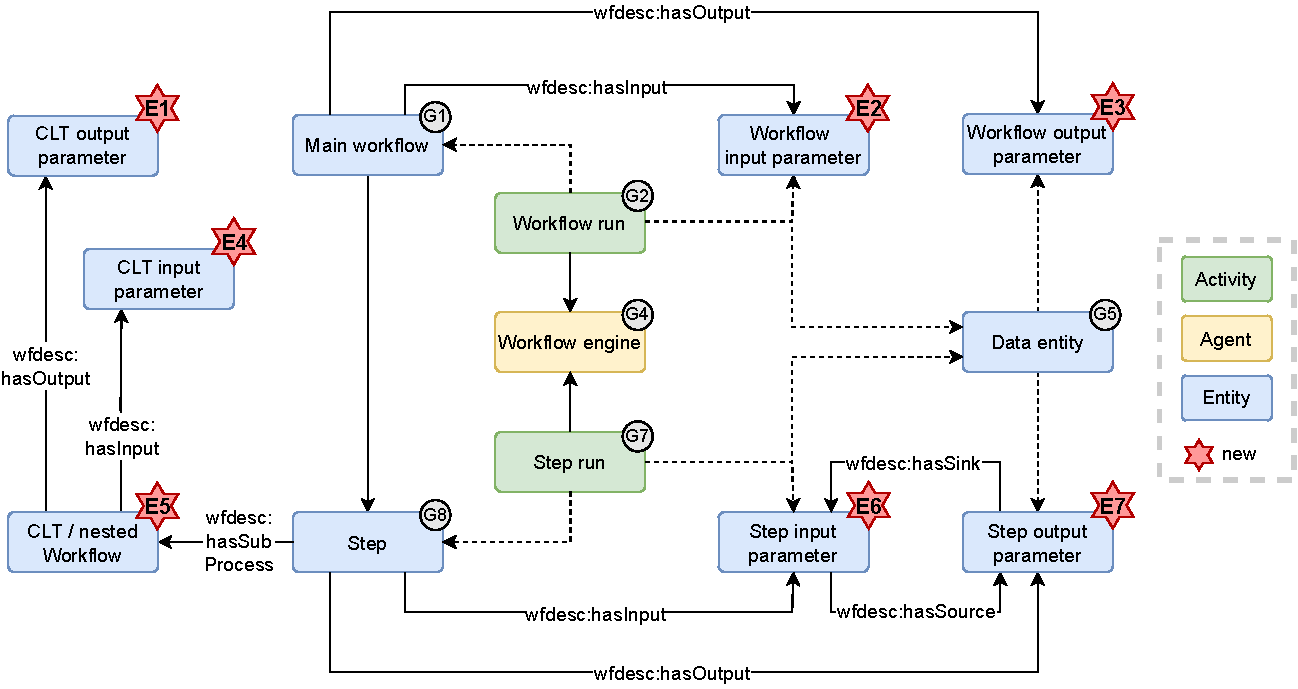
\includegraphics[width=0.99\textwidth]{rdf_extension/CWLProv_graph_extended.pdf}
    \caption{The RDF provenance graph, now extended with \emph{CommandLineTools} and parameter entities. Red stars mark nodes which are part of the design extension. Parameters are linked to their \emph{Workflow}, \emph{CommandLineTool} or step via \emph{wfdesc:hasInput} and \emph{wfdesc:hasOutput}. Node G5 represents both input and output data entities. The data flow between steps is represented via \emph{wfdesc:hasSink} and \emph{wfdesc:hasSource}. Steps are linked to their underlying tools via \emph{wfdesc:hasSubProcess}.}
    \label{fig:cwlprov_graph_new}
\end{figure*}



\begin{figure}[ht]
    \centering
    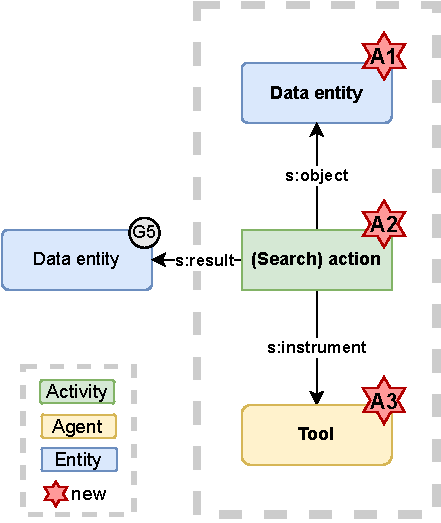
\includegraphics[width=0.4\textwidth]{rdf_extension/CWLProv_graph_extended_actions.pdf}
    \caption{Actions represented in RDF provenance graph. Workflow input datasets (\textbf{G5}) are connected to the Actions (\textbf{A2}) which produced them via \emph{s:result}. In addition, Actions can have properties such as \emph{object} (\textbf{A1}) and \emph{instrument} (\textbf{A3}).  }
    \label{fig:cwlprov_graph_actions}
\end{figure}

In Section \emph{\nameref{sec:cwlprov_evaluation}}, we analyzed CWLProv for the representation of the provenance taxonomy we defined in \emph{\nameref{sec:user_req}}. Based on this analysis, we concluded that not all provenance components were sufficiently represented in a structured format. Specifically, we found that although certain metadata was part of \emph{primary-job.json} and \emph{packed.cwl}, these annotations were not represented in RDF format.

In this section, we propose an extension of the design of the CWLProv provenance graph, which can at least represent the values for already supported metadata fields and can also be extended later with other metadata. %In this way, we (partially) answer \ref{rq:improve}.

Here, we are only concerned with the representation of this information, if it exists. Mechanisms for the collection of the metadata (whether it be manually or automated), are considered out of scope for this paper. 

In Section \emph{\nameref{sec:ext_reqs}}, we first describe the requirements and principles which we used in this design. Subsequently, in Section \emph{\nameref{sec:ext_overview}}, we give a high-level overview of the design. We then give recommendations for specific terms and vocabulary which can be used for the metadata fields \emph{doc}, \emph{label}, \emph{intent}, and \emph{format} which are part of v1.2 of the CWL Standards (Section \emph{\nameref{sec:ext_details}}). We describe how we have partially realized this design in \emph{cwltool} (Section \emph{\nameref{sec:realization}}). Finally, we provide a list of SPARQL queries in Section \emph{\nameref{sup:sparql}}.
\stodor{keep the analysis in?}

\subsection{Requirements and principles}
\label{sec:ext_reqs}
For this design, we reuse principles \ref{pr:bioschemas} and \ref{pr:current_standards}. In addition, the RDF extension should adhere to four requirements.

\begin{enumerate}[label=\textbf{PR\arabic*}]
    \item \label{pr:metadata_fields} Represent the annotations that are supported in CWL workflows according to the CWL standards v1.2, summarized in Table \ref{tab:metadata_fields}.
    \item \label{pr:input} Represent the annotations for \emph{Files} and \emph{Directories} proposed in Section \emph{\nameref{sec:annot_cwl_now}}.
    \item \label{pr:execution} Represent the annotations for a collection of input values proposed in Section \emph{\nameref{sec:annot_cwl_now}}.
    \item \label{pr:actions} Represent the annotations for Actions proposed in Section \emph{\nameref{sec:annot_new_cwl}}.
\end{enumerate}

\subsection{High-level overview}
\label{sec:ext_overview}
In this section, we present a high-level overview of the extended provenance graph and link it to the requirements defined in Section \emph{\nameref{sec:ext_reqs}}.

\subsubsection{Representation of CWL metadata fields}

\begin{table}[bt!]
\caption{Metadata fields in CWL Standards v1.2. \emph{format} is only allowed for parameters of type File or File array.}\label{tab:metadata_fields}
\begin{tabularx}{\linewidth}{L l l l l}
\toprule
Workflow component & label & doc & intent & format \\
\midrule
% Widgets & 42 & Over-supplied\textsuperscript{*} \\
% Gadgets & 13 & Under-supplied \\
Workflow & \textbullet & \textbullet & \textbullet & ~\\ %\hline
WorkflowStep & \textbullet & \textbullet & ~ & ~\\ %\hline
CommandLineTool & \textbullet & \textbullet & \textbullet & ~\\ %\hline
ExpressionTool & ~ & ~ & \textbullet & ~\\ %\hline
WorkflowInputParameter & \textbullet & \textbullet & ~ & \textbullet\\ %\hline
WorkflowOutputParameter & \textbullet & \textbullet & ~ & \textbullet\\ %\hline
WorkflowStepInput & \textbullet & ~ & ~ & ~\\ %\hline
WorkflowStepOutput & ~ & ~ & ~ & ~\\ %\hline
CommandInputParameter & \textbullet & \textbullet & ~ & \textbullet\\ %\hline
CommandOutputParameter & \textbullet & \textbullet & ~ & \textbullet\\ %\hline
\bottomrule
\end{tabularx}
\end{table}

Figure \ref{fig:cwlprov_graph_new} shows how we extended the provenance graph to represent all current metadata fields (\ref{pr:metadata_fields}). \textbf{In the new graph, every workflow component in Table \ref{tab:metadata_fields} is represented as a distinct entity, and interrelated with terms from the \emph{wfdesc} ontology (\ref{pr:bioschemas}).} 
We added entities describing the CWL tools that are run by the steps (\textbf{E5}) and linked them to their input (\textbf{E4}) and output parameters (\textbf{E1}) via \emph{wfdesc:hasInput} and \emph{wfdesc:hasOutput}. We connected the steps (\textbf{G8}) and tools via \emph{wfdesc:hasSubProcess}. In addition, we linked the step parameters (\textbf{E6}, \textbf{E7}) together via \emph{wfdesc:hasSource} and \emph{wfdesc:hasSink} to express the data flow between the steps.

In CWLProv 0.6.0, the execution of nested workflows is described in separate RDF documents. \textbf{Following the same strategy, we recommend to only represent top-level parameters of nested workflows in the primary provenance graph.} More detailed annotations can be represented in the separate RDF documents which describe the nested workflows.

\subsubsection{Representation of input data annotations}
This structure depicted in Figure \ref{fig:cwlprov_graph_new} also supports representation of the input data annotations described in \emph{\nameref{sec:annot_cwl_now}} (\ref{pr:input}), by transferring them to the data entities they describe (\textbf{G5}). 


\subsubsection{Representation of configuration settings annotations} Annotations describing a collection of parameters (\ref{pr:execution}) are specific to the workflow execution. Therefore, we recommend that these annotations are transferred to the entity in the provenance graph describing the workflow execution (\textbf{G2}).

\subsubsection{Representation of input data history}
In the annotation scheme described in Section \emph{\nameref{sec:annot_new_cwl}}, the history of (processed) input data is expressed through \emph{Actions}. Figure \ref{fig:cwlprov_graph_actions} presents their representation in RDF (\ref{pr:actions}). 
Actions (\textbf{A2}) are performed on objects, which are data entities not aggregated in the CWLProv RO (\textbf{A1}). Actions can have additional properties such as Tools (\textbf{A3}) or other annotations as summarized in Table \ref{tab:action_schemaorg}. They are connected to input data entities (\textbf{G5}) via \emph{s:result}. 



\subsection{Details of the design}
\label{sec:ext_details}
Here, we move from the structure of the provenance graph to the annotations that now can be attached to the newly added entities and with which terms they should be represented.

First, we describe which terms to use for the CWL-specific metadata fields \emph{doc}, \emph{label}, \emph{format}, and \emph{intent}.

Although we could use the exact terms with \emph{cwlprov} prefix, we aim for interoperability with other provenance representations, such as the RO-Crate specification. Therefore, we reuse Schema.org terms, and because this is in agreement with our annotation scheme:

\begin{itemize}
    \item \textbf{doc}: http://schema.org/description
    \item \textbf{label}: http://schema.org/name
    \item \textbf{format}: http://schema.org/encodingFormat
    \item \textbf{intent}: http://schema.org/featureList
\end{itemize}

\textbf{In addition, we recommend that custom annotations attached to workflow components and input objects are transferred as they are.} We make an exception for \emph{s:additionalType}, for which the value can be added to the \emph{types} of the entity it describes, instead of being literally transferred as \emph{s:additionalType}.

When entities are described with nested annotations (e.g. \emph{s:citation}), we recommend to make this a separate entity in the graph instead of a nested annotation, in compliance with the PROV data model (\ref{pr:bioschemas}).

\subsection{Partial realization in \emph{cwltool}}
\label{sec:realization}
\todorenske{Update, when this is published there should be full support in cwltool.}
Because of time constraints, we could only partially realize the provenance graph extension in \emph{cwltool}. At the time of writing, annotations directly associated with inputs of type \emph{File} and \emph{Directory}, as exemplified in \emph{\nameref{sec:annot_fair}}, are propagated to the RDF provenance record. However, annotations of the collection of input parameter values (\emph{\nameref{sec:annot_actions}}) or annotations under \emph{cwlprov:prov} (\emph{\nameref{sec:annot_new_cwl}}), are currently not represented in RDF.

\subsection{Conceptual analysis of the design extension}
\label{sec:ext_analysis}

\todorenske{leave in?}
To test the extended design, we analyzed the RDF provenance graph which would have been associated with the epitope prediction workflow we used as an example in this thesis. The elements of the design which were not yet realized in \emph{cwltool}, we emulated via manual annotations of the document. 

\subsubsection{SPARQL queries.}

\todorenske{replace with all sparql queries}
Here, we present two example SPARQL queries we issued on the emulated extended provenance graph. The first (\textbf{Q1}) extracts the DOIs of all publications which were the citations of the used inputs.

The second (\textbf{Q2}) lists the formats for every file for which this is specified.

\clearpage
% \section{Taxonomy}

\subsection{\ref{tax:context}: Definition of metadata for scientific context}
\label{sec:reasoning_reqs}

In ??, we presented scientific context (\ref{tax:context}) as one of the aspects that should be present in the collected provenance. In this section, we elaborate on what we mean with scientific reasoning and how it should be incorporated in provenance.

\textbf{Why:} Representing the scientific thinking process in provenance is meant to make the connection between the article advertising the research and the research itself, contained in the RO. This connection is bidirectional: ROs can be used as a guide during manuscript writing as well as for providing context for a third party who has read the paper and wants to understand the analysis in more depth.

\textbf{What:} The scientific context covers many aspects of the research, from the reasons why particular input data and parameter settings were chosen \cite{committeeonreproducibilityandreplicabilityinscienceReproducibilityReplicabilityScience2019}, to the design of the workflow (why particular steps were included), to the rationale for the study and the overall hypothesis of the research \cite{belhajjameResearchObjectSuite2014}\cite{grykWorkflowsProvenanceInformation2017}. Even negative results can be reported and explored strategies which did not work can be included \cite{stoddenEnhancingReproducibilityComputational2016}. In addition, it can include the interpretation of the results and their implications on the field (or maybe the output of an intermediate step warrants the inclusion of another preprocessing step).

\textbf{How:} We classify scientific context into 3 components:
\begin{enumerate}[label=\textbf{SC\arabic*}]
    \item \textbf{Workflow design}. Annotations on the design of the workflow and its components. Purpose of the workflow, why steps were included or excluded, the meaning of particular input parameters, etc. \label{req:sr_wf}
    \item \textbf{Entity annotations}: The meaning of individual input and output data entities. Why were they chosen? How are the results interpreted? \label{req:sr_data}
    \item \textbf{Workflow execution annotations}: Annotations about a set of parameters in a particular workflow run. Allows to distinguish between the ROs of multiple workflow runs. \label{req:sr_ex}
\end{enumerate}

% \subsection{\ref{tax:data}: Definition of metadata for data}
\label{sec:data_reqs}

In this section, we describe which metadata should be attached to data entities (\ref{tax:data}) in the provenance record. 

\textbf{What:} We mean not only input data, but also (intermediate) output data.

\textbf{Why:} Metadata associated with data entities can have at least two purposes:
\begin{itemize}
    \item \textbf{To explain the meaning and context of the data.} The context of the data should be described, because others need to be able to assess the appropriateness of the data for the purpose of the computational analysis. \textit{In the case of the epitope prediction workflow, it is important to understand the composition of the training set, since this is highly influential on the performance and applicability of the model.}
    \item \textbf{To describe data which is not contained in the RO.} To reduce RO size, or because the data cannot be shared for privacy reasons (it is proprietary or in other ways non-public), data may not be present in the RO but stored in an external repository. Characteristics of the data may still be included which provide information, to make sure that the data in the repository is the same as which was used in the original analysis. \textit{Use case \ref{uc:service} is an example where limiting the size of the RO may be desirable. Instead, the RO could contain references to datasets which are too large and are instead stored in an external repository.}
\end{itemize}

\textbf{How:} We identify 4 categories of data metadata which should be represented based on these two reasons. Here we link them to established recommendations and best practices for data citation, according to the FORCE11 Data Citation Principles \cite{datacitationsynthesisgroupJointDeclarationData2014}, which are based on the FAIR principles \cite{wilkinsonFAIRGuidingPrinciples2016}.

\begin{enumerate}[label=\textbf{D\arabic*}]
    \item \textbf{Identification}: PID, version, name and description of the dataset. Preferred citation of the data. \emph{When the data is not FAIR:} URL and download date as an alternative for PID and version. \emph{When the dataset is a subset of a larger collection (e.g. a database):} PID of database, database version and download date, and the query or filtering strategy which produced the dataset. \label{req:data_id}
    \item \textbf{File characteristics}: Filename, format, creation and last modification timestamps, size, and checksum. \label{req:data_char}
    \item \textbf{Access}: URL to a downloadable form of the data. License. \label{req:data_access}
    \item \label{req:data_mapping} \textbf{Mapping}: The workflow and step parameters for which the data is an input or output.
\end{enumerate}

% \subsection{\ref{tax:software}: Definition of metadata for software}
\label{sec:software_reqs}

In this section, we elaborate on the representation of software in the provenance record (\ref{tax:software}). 

\textbf{What:} In particular, we mean the command-line programs directly orchestrated by the workflow. However, these principles also apply to the workflow itself (\Cref{sec:wf_reqs}), the workflow engine (\Cref{sec:execution_reqs}), and computational environment (\Cref{sec:env_reqs}).

\textbf{Why:} There are two main reasons why software should be described with metadata:

\begin{itemize}
    \item \textbf{Obtaining identical results in a re-execution may be highly dependent on the version of the tools used.} This is important when reproducing the workflow. 
    \item \textbf{The original software may not be available or executable in the future.} In this case, the software should be sufficiently described for others to choose a suitable equivalent. 
\end{itemize}

\textbf{How}: We identify 3 categories of software characteristics which should be included in the provenance. Here we link them to established recommendations and best practices for software citation, according to the FORCE11 Software Citation Principles \cite{smithSoftwareCitationPrinciples2016}, which were adapted from the FORCE11 Data Citation Principles.

\begin{enumerate}[label=\textbf{SW\arabic*}]
    \item \textbf{Identification}: PID, name, version, release date and description of the software. Preferred citation. \textit{When the software is not FAIR:} URL of repository, download date and/or git commit hash as substitute for PID, version or release date. \label{req:sw_id}
    \item \textbf{Documentation}: URL of documentation or other metadata which is important to make informed use of the tool. URL to repository with source code of the software. \label{req:sw_doc}
    \item \textbf{Access}: URL to downloadable, executable form of the software. License. \label{req:sw_access}
\end{enumerate}


% \subsection{\ref{tax:wf}: Definition of metadata for workflow}
\label{sec:wf_reqs}

In this section, we describe the metadata that is associated with the workflow (\ref{tax:wf}). 

\textbf{What}: We define workflow here as the documents described in CWL (for other workflows, this would be the top-level script, not the underlying software that it controls). Hence the workflow comprises the main workflow description and the \emph{CommandLineTool} and nested \emph{Workflow} descriptions. 

\textbf{Why}: Workflows provide both a high-level overview of the analysis as well as details which are difficult to convey in a textual format in the Methods section of a scientific article \cite{gilAutomatingDataNarratives2017}. In addition, workflows are software which should be preserved and reused \cite{gobleFAIRComputationalWorkflows2020}. 

\textbf{How}: The metadata associated with workflows comprise general software metadata, in addition to workflow-specific information. 
\begin{enumerate}[label=\textbf{WF\arabic*}]
\item \textbf{General software metadata}: At workflow and step level, according to \Cref{sec:software_reqs}. \label{req:wf_all}
\item \textbf{Parameters}: Type, format, and description, at workflow and step-level. \label{req:wf_param}
\item \textbf{Requirements}: Software and hardware resources which are required to execute the workflow or workflow steps. \label{req:wf_resources}
\end{enumerate}


% \subsection{\ref{tax:env}: Definition of metadata for computational environment}
\label{sec:env_reqs}

In this section, we describe the requirements for computational environment (\ref{tax:env}).

\textbf{What}: Environment encompasses both software and hardware infrastructure, and may be part of a software container.

\textbf{Why}: Information about the computational environment is important for reproducing the workflow (\ref{uc:reproducing}). 

\begin{itemize}
    \item \textbf{Required resources:} Details about the resources available on the system which executed the original analysis can give an indication of what is necessary to rerun the workflow, even if this is not documented in the workflow description.
    \item \textbf{Debugging:} The generated output (or executability) of a step may be sensitive to specific versions of the tool orchestrated by the step or its dependencies.
\end{itemize}

\textbf{How}: We discriminate between three components of the computational environment:
\begin{enumerate}[label=\textbf{ENV\arabic*}]
    \item \textbf{Software}: software (dependencies), operating system. Dependencies could comprise all installed software (might contain much redundant information if a step was not executed in a software container), or the dependencies of the software which is run (which may be difficult to identify). Should follow the requirements as described in \Cref{sec:software_reqs}. \label{req:env_software}
    \item \textbf{Hardware}: Available RAM, storage, number and type of CPUs and GPUs. Network access. \label{req:env_hardware}
    \item \textbf{Container image}: Image name, tag and digest (because names and tags are not stable). Additional metadata (extracted from image labels), contents of Dockerfile (if built from Dockerfile), and general requirements for software as described in \Cref{sec:software_reqs}. \label{req:env_image}
\end{enumerate}

% \subsection{\ref{tax:execution}: Definition of metadata for execution details}
\label{sec:execution_reqs}

In this section, we define the final element of our provenance taxonomy: execution details (\ref{tax:execution}).

\textbf{What}: Executions are everything that is related to the analysis but which is not covered by the other categories. They constitute pure retrospective provenance: a record of what actually happened during the workflow run. 

\textbf{How}: We distinguish four components in this category:

\begin{enumerate}[label=\textbf{EX\arabic*}]
    \item \textbf{Timestamps}: When the workflow was executed, at step-granularity. The timestamps can be helpful when files were downloaded during the execution, especially from a database which does not have clear versions (SAbDab). In addition, the duration of the execution may be important during workflow development (test different settings) and when reproducing the workflow. \label{req:ex_time}
    \item \textbf{Consumed resources}: The resources used during execution, at step-granularity. This is different from what was described in \Cref{sec:env_reqs}, because there we only described what was available, not what was actually used. \label{req:ex_resources}
    \item \textbf{Workflow engine}: Software, therefore with same metadata as general software entities (\Cref{sec:software_reqs}).\label{req:ex_engine}
    \item \textbf{Human agent}: At a minimum, a PID such as ORCID should be included, or name and email of the person who ran the workflow. These details may be important for attribution (\ref{uc:writing}), and can also be used by third parties to ask further questions about the research.  \label{req:ex_human}
\end{enumerate}


\onecolumn
\section{SPARQL queries}
\label{sup:sparql}

\subsection{How to run the queries}

\begin{verbatim}
import rdflib
from rdflib.plugins.sparql import prepareQuery
from rdflib.namespace import Namespace
import pandas as pd

def run_query(rdf_file, query_file, namespaces):
    """
    rdf_file = RDF file; query_file = path to sparql query file; namespaces = Namespace object for every prefix in the SPARQL query.
    """
    g = rdflib.Graph()
    g.parse(rdf_file)
    with open(query_file, 'r')  as f:
        query_string = f.read()
        query = prepareQuery(
            queryString = query_string,
            initNs = namespaces,
        )

    print(f"SPARQL QUERY IS:\n{query}")
    
    qres = g.query(query)
    
    results = pd.DataFrame(qres.bindings).map(str).rename(columns=str)
    return results

def extract_wf_namespace(rdf_file):
    """
    Function which extracts namespace from CWLProv RDF provenance graph.
    """
    g = rdflib.Graph()
    g.parse(rdf_file)
    namespaces = list(g.namespaces())
    wf_namespace = ""
    for ns in namespaces:
        (prefix, namespace) = ns
        if prefix == "wf":
            wf_namespace = namespace

    return wf_namespace

provenance_file = "/path/to/provenance/file.ttl"
query_file = "/path/to/sparql/query/file.sparql" # file with any of the SPARQL queries listed in the section below

SCHEMA = Namespace("http://schema.org/")
WFDESC = Namespace("http://purl.org/wf4ever/wfdesc#")
wf_namespace = extract_wf_namespace(provenance_file)

namespaces = {"wf": wf_namespace, 
              "wfdesc": WFDESC,
              "schema": SCHEMA }

# How to run the query
response = run_query(provenance_file, query_file, namespaces)
\end{verbatim}

\subsection{SPARQL queries}

\noindent
\textbf{Return the \emph{doc}, \emph{label} and \emph{intent} fields of the main workflow.}

\lstinputlisting[basicstyle=\footnotesize]{sparql_queries/queries/wf_metadata_fields.sparql}

\noindent
\textbf{List \emph{doc} and \emph{label} fields of all \emph{WorkflowSteps} in the main workflow.}


\lstinputlisting[basicstyle=\footnotesize]{sparql_queries/queries/wf_step_metadata_fields.sparql}

\noindent
\textbf{Return the \emph{doc}, \emph{label} and \emph{intent} fields of every command-line tool or nested workflow that is run by each of the steps.}

\lstinputlisting[basicstyle=\footnotesize]{sparql_queries/queries/clt_nested_wf_metadata_fields.sparql}

\noindent
\textbf{List \emph{doc}, \emph{label}, \emph{format} fields of all input parameters of main workflow.}

\lstinputlisting[basicstyle=\footnotesize]{sparql_queries/queries/wf_input_params_metadata_fields.sparql}

\noindent
\textbf{List \emph{doc}, \emph{label}, \emph{format} fields of all output parameters of main workflow.}

\lstinputlisting[basicstyle=\footnotesize]{sparql_queries/queries/wf_output_params_metadata_fields.sparql}

\noindent
\textbf{List \emph{doc}, \emph{label}, \emph{format} fields of all input parameters of nested \emph{Workflows}/\emph{CommandLineTools}.}

\lstinputlisting[basicstyle=\footnotesize]{sparql_queries/queries/clt_nested_wf_input_params_metadata_fields.sparql}

\noindent
\textbf{List \emph{doc}, \emph{label}, \emph{format} fields of all output parameters of nested \emph{Workflows}/\emph{CommandLineTools}.}


\lstinputlisting[basicstyle=\footnotesize]{sparql_queries/queries/clt_nested_wf_output_params_metadata_fields.sparql}

\end{document}
